%%____________________________________________________________________________||

%%____________________________________________________________________________||
\RCS$Revision: 273188 $
\RCS$HeadURL: svn+ssh://svn.cern.ch/reps/tdr2/notes/AN-15-004/trunk/AN-15-004.tex $
\RCS$Id: AN-15-004.tex 273188 2015-01-08 15:07:24Z alverson $

%%____________________________________________________________________________||
\newlength\cmsFigWidth
\ifthenelse{\boolean{cms@external}}{\setlength\cmsFigWidth{0.85\columnwidth}}{\setlength\cmsFigWidth{0.4\textwidth}}
\ifthenelse{\boolean{cms@external}}{\providecommand{\cmsLeft}{top\xspace}}{\providecommand{\cmsLeft}{left\xspace}}
\ifthenelse{\boolean{cms@external}}{\providecommand{\cmsRight}{bottom\xspace}}{\providecommand{\cmsRight}{right\xspace}}

%%____________________________________________________________________________||
\cmsNoteHeader{AN-15-004}

%%____________________________________________________________________________||
\title{PHYS14 exercise for supersymmetry searches with the $\alpha_\rm T$ variable}

%%____________________________________________________________________________||
\author[imperial]{M.~Baber}
\author[imperial]{R.~Bainbridge}
\author[imperial]{O.~Buchm\"uller}
\author[imperial]{M.~Citron}
\author[imperial]{A.~Elwood}
\author[bristol]{H.~Fl\"acher}
\author[rochester]{A.~Garcia-Bellido}
\author[rochester]{K.H.~Lo}
\author[bristol]{C.~Lucas}
\author[imperial]{S.A.~Malik}
\author[imperial]{B.~Penning}
\author[bristol]{T.~Sakuma}
\author[bristol]{D.~Smith}
\author[imperial]{A.~Tapper}

\address[imperial]{Imperial College, London, UK}
\address[bristol]{University of Bristol, UK}
\address[rochester]{University of Rochester, NY, US}

%%____________________________________________________________________________||
\date{\today}

%%____________________________________________________________________________||
\abstract{This note summarizes a PHYS14 exercise for supersymmetry
searches with with the $\alpha_{\rm T}$ variable and a trigger
preparation for the searches for the LHC Run-2.}

%%____________________________________________________________________________||
\hypersetup{
  pdfauthor={Mark Baber, Robert Bainbridge, Oliver Buchmueller,
  Matthew Citron, Adam Elwood, Henning Flaecher, Aran Garcia-Bellido,
  Kin Ho Lo, Chris Lucas, Sarah Alam Malik, Bjoern Penning, Tai Sakuma,
  Dominic Smith, Alex Tapper.},
  pdftitle={PHYS14 exercise for supersymmetry searches with
  with the AlphaT variable},
  pdfsubject={CMS, jets, missing transverse momentum, supersymmetry, AlphaT},
  pdfkeywords={CMS, jets, missing transverse momentum, supersymmetry, AlphaT},
}

%%____________________________________________________________________________||
\maketitle

%%____________________________________________________________________________||
\tableofcontents

%%____________________________________________________________________________||
%%____________________________________________________________________________||
\section{Introduction}
\label{sec:intro}


In this note, we summarize the PHYS14 exercise [REF] for the \alphat
analysis, which searches for signatures of physics beyond the standard
model in events with jets and missing transverse momentum (MET). This
analysis uses the kinematic variable \alphat in selecting events with
missing transverse momentum.

With this variable \alphat, CMS has been searching for supersymmetry
(SUSY) in proton-proton collisions data collected during LHC Run 1. With
data at a centre-of-mass energy of 7 TeV collected in 2010 and 2011, the
\alphat analysis has excluded a large parameter space of the constrained
minimal supersymmetric extension of the standard model (CMSSM)
\cite{Khachatryan:2011tk, Chatrchyan:2011zy, Chatrchyan:2012wa} and a
parameter space of simplified models \cite{Chatrchyan:2012wa}. With data
at a centre-of-mass energy of 8 TeV collected and promptly reconstructed
in 2012, the \alphat analysis further excluded a parameter space of
simplified models \cite{Chatrchyan:2013lya}. Additional sets of data
which were collected in 2012 but were reconstructed later during the LHC
Long Shutdown 1 (LS1) are called the ``parked data'', which contain data
for events triggered with lower energy thresholds. The review of the
\alphat analysis of the parked data \cite{CMS_AN_2013-366} is ongoing.
The search strategy in this note is an extension of that in Ref.
\cite{CMS_AN_2013-366}.

After two years of the LS1, in the middle of 2015, LHC will start its
Run 2 and deliver proton-proton collisions to CMS at a higher
centre-of-mass energy of 13 TeV. It is highly motivated to continue the
search for supersymmetry at this higher energy. The \alphat analysis is
particularly suited for this search and has potential for discovery in
early data. The higher energy collision considerably increases the
production cross sections of heavy particles. The reconstruction of
missing transverse momentum in different collider environment or at new
collider energy is typically very challenging and often requires an
extended period of the development. However, the variable \alphat can
effectively select events with missing transverse momentum without
directly using the reconstructed missing transverse momentum.

The production of dark matter at LHC Run 2 has been predicted by many
models of physics beyond the standard model, by both supersymmetric and
non-supersymmetric models. The variable \alphat can be also effective to
select events that potentially contain dark matter produced in the
collisions. In Run 2, we will extend the \alphat analysis to include the
collider dark matter search.

The PHYS14 exercise, which started in October 2014 and will conclude in
February 2015, is a preparation for LHC Run 2 carried out in the CMS
collaboration. This exercise is particularly focused on the preparation
of physics analyses. In this exercise, we analyzed events which were
simulated under conditions anticipated in early LHC Run 2, e.g, the
centre-of-mass energy, the bunch-spacing, the number of the interactions
per bunch crossing. We have derived expected exclusion limits on
parameter spaces of simplified models.

Section \ref{sec:strategy} discusses changes in the search methods that
we are planning to make in Run 2. Section \ref{sec:dm} introduces the
dark matter searches. Section \ref{sec:datasets} lists the data sets
used in this note. Section \ref{sec:triggers} describes the preparation
of the triggers for Run~2. Section \ref{sec:objects} defines the physics
objects used in this note. Section \ref{sec:selection} describes how
events are selected. Section \ref{sec:physics} shows the performance of
the event selection. Section \ref{sec:background} discusses the
background estimation. Section \ref{sec:sensitivity} discusses the
search sensitivity. Section \ref{sec:summary} summarizes this exercise.




%%____________________________________________________________________________||

%%____________________________________________________________________________||
\section{Analysis strategy}
\label{sec:strategy}

\textbf{FIXME: We either want to modify the content or simply put the relevant information described here somewhere else} \\

\subsection{The analysis during Run~1}

While the analysis strategy has evolved significantly prior to and
during Run~1, certain design features have remained central to the RA1
analysis throughout the run. These features, along with some of the
more important recent developments, are outlined below.

{\bf Model-independent search for new physics:}

The analysis is designed to be sensitive to a range of beyond standard
model (BSM) physics scenarios with signatures that are characterised
by jets and significant \met in the final state. The search is one of
the original Reference Analyses (RAs) that formed the basis of the CMS
SUSY search program at the beginning of Run~1. The program was
designed to be inclusive, model-independent (as much as possible), and
topology-based. 

The current incarnation of the RA1 search still retains its generic,
inclusive nature. A binned signal region, defined by a set of
inclusive selection criteria, is employed to provide sensitivity to a
range of new physics models. By the end of Run~1, three discriminating
variables were used to categorise signal event candidates: \scalht,
\njet, and \nb. In the case of SUSY, this choice of variables provides
sensitivity to the direct pair-production of all flavours of squarks,
as well as pair-produced gluinos and their decays via, again, all
favours of squarks. The large dymamic range in \scalht provides
sensitivity to a large range of mass splittings between the parent
sparticle and the LSP.

{\bf Robust performance under Start-Up conditions:}

The search relies on the \alphat variable, which strongly suppresses
the dominant background of multijet production from QCD, while
maintaining acceptance to new physics signatures with genuine \met in
the final state. At the beginning of Run~1, the \alphat variable was
chosen because it was shown to be extremely effective at operating
under Start-Up conditions, when the beam conditions and detector
performance were poorly understood. For example, multijet
events with significant \met from jet mismeasurements due to
instrumental effects are penalised to lower values of \alphat, hence
the variable exhibits an intrinsic robustness against potential
sources of ``fake'' \met.

% Further, the analysis did not use directly the \met variables and
% relied instead solely on calorimeter-based jets (with relatively
% high thresholds of \Pt > 50\gev) to

While the Collaboration now has a deep understanding of the detector
performance under Run~1 conditions, the strategy we employ will still
be very relevant when exploring the new high-energy, high-luminosity
frontier expected in Run~2.

{\bf Inclusive trigger strategy with low thresholds:}

The trigger strategy has made use of the \alphat variable at the HLT
since 2011. Given the rejection power of \alphat for multijet events,
we employ this variable (crossed with \scalht) at the trigger level,
which allows to push to lower thresholds for a given trigger rate with
respect to other discriminating variables typically used in jets +
\met searches (\eg \met, \mht, etc). A suite of \scalht-\alphat cross
triggers allowed the RA1 search to push as low as $\scalht > 200\gev$
and (effectively) $\mht \gtrsim 100\gev$ at the trigger, and as low as
$\scalht > 200\gev$ and (effectively) $\mht \gtrssim 130\gev$ in the
signal region definition, with near-maximum signal efficiency at the
cost of $\sim25$~Hz (of which $\sim$15 was ``parked'').

{\bf Multijet-free signal region.}

As the analysis has evolved, the event selection has been tailored to
provide a multijet-free sample of signal event candidates. This is
achieved by applying a \scalht-dependent \alphat threshold, tuned to
suppress the multijet contribution to the sub-percent level with
respect to the total background counts per signal region bin. This is
extremely important for the lowest \scalht bins, which provide a
significant contribution to the overall sensitivity to compressed SUSY
or Dark Matter models.

{\bf Access to new physics via initial state radiation:}

The analysis acceptance to very compressed SUSY models relies not on
the detection of very soft objects (often failing acceptance cuts)
produced in the decay of the sparticles, but instead on the presence
of jets from initial state radiation. The signal acceptance times
efficiency for this mechanism is typically at the sub-percent level.
Further, the signal is characterised by a very broad shape in \scalht,
with significant counts at low \scalht, as well low values of \njet,
\nb, and \mht. Hence, the highest signal counts are typically found in
the bins with the highest background counts, typically populated by
events from W + jets and Z$\ra\nu\nu$ + jets, which results in a poor
S/B. Hence, the signal shape over many bins has to be considered in
order to achieve reasonable sensitivity to such signatures. One
distinguishing feature with respect to the SM backgrounds, which is
most pronounced for (near-)degenerate spectra, is that while the
values of \scalht and \mht are typically small, the ratio $\mht /
\scalht$ is large with respect to SM backgrounds.

This mechanism of signal acceptance was the focus of the ``parked
analysis'' in Ref~\cite{CMS_AN_2013-366}. While the interpretations of
this result focused on strongly-produced compressed SUSY models, the
same mechanism can be used to access the direct production of a Dark
Matter candidate, as detailed in Sec.~\ref{sec:dm}. Sensitivity to this
class of models relies heavily on tight background control and low
thresholds. This is the motivation for the strategies of developing
high-performance triggers with low thresholds, tuning the event
selection to provide a multijet-free signal region, and relying on a
large ensemble of closure tests in data to demonstrate excellent
control of the non-multijet backgrounds in the signal region.

{\bf Data-driven background estimation methods and closure tests:}

The analysis relies on multiple data control samples to predict the
non-multijet backgrounds. The control samples have a composition very
similar to the signal region, cover a very similar kinematic phase
space, have a large acceptance, and are signal-depleted. The analysis
relies on transfer factors constructed from MC to extrapolate from the
control regions to the signal region. The extrapolation is minimised
by using identical binning in all samples. Potential residual biases
in the transfer factors, \eg from MC mismodelling, are probed though a
large ensemble of closure tests performed between numerous data
control sub-samples. Several hundred statistically independent tests
are performed, which cover a wide range of potential biases. 

These closure tests are one of the most crucial components of this
analysis, as they provide an understanding of the reliance on MC (in
the form of ratios, \ie transfer factors) that is {\it founded on
  comparison with data}. Any potential biases or dependencies on the
discriminating variables used to categorise the signal events must be
understood prior to unblinding the signal region. There are concrete
examples in the past when the closure tests have revealed problems,
which had to be understood and solved prior to continuing with the
analysis.

In the absence of any significant biases, the closure tests are then
used to determine systematic uncertainties on the transfer factors,
which are propagated through to the analysis result via the likelihood
model. These systematic uncertainties are therefore motivated through
comparisons with control data and are, ultimately, statistically
limited by the data counts in the control samples. With increasing
integrated luminosity, we expect the closure tests to be increasingly
statistically-significant probes of potential biases and, in the
absence of bias, the systematic uncertainties will correspondingly
reduce.

\subsection{Developments with respect to the Run~1 analysis}
\label{sec:changes}

We plan to build on the experience gained during Run~1 and develop the
analysis to provide improved sensitivity to a range of new physics
models. These developments fall broadly under three categories:

\begin{itemize}
\item general optimisations concerning event reconstruction and
  selection;
\item improvements in the sensitivity to heavy objects, such as gluinos;
\item improvements concerning compressed SUSY and Dark Matter
  models. 
\end{itemize}

Some of these changes have already been implemented, while some are
still under study. The status will be noted at appropriate points in
this document. A summary of these changes are listed below. This list
is not exhaustive and some developments are subject to change.

{\bf Particle Flow event reconstruction:}

The analysis will switch from relying on jets reconstructed solely
from calorimeter information to the use of jets from the Particle Flow
(PF) reconstruction algorithm. This change will provide performance
improvements for jet-based variables (including \scalht, \mht, and
\alphat) and, in particular, better mitigate any effects relating to
pileup.

{\bf General event selection optimisation:}

In addition to the switch to PF, all event selection criteria for the
signal region and control samples are currently under review. The jet
\Pt threshold is no longer scaled at low \scalht as during Run~1, and
the binning in \scalht has been simplified. The binning choice in the
signal region will evolve with integrated luminosity.  We also plan to
investigate developments concerning lepton isolation and boosted
objects.

{\bf Trigger strategy:}

The trigger strategy is similar to that of Run~1, which will continue
to rely on a suite of \scalht-\alphat cross triggers at the HLT. The
trigger decision is now based on PF jets, rather than
calorimeter-based jets as during Run~1. The aim is to maintain the
thresholds used at the end of Run~1, which fall in the range of $200 <
\scalht < 400\gev$ and $0.57 > \alphat > 0.51$. MC-based studies have
revealed this appears to be achievable. Studies are ongoing to further
mitigate any performance degradation due to pileup.

The highest \scalht bins in the analysis will be seeded by the lowest
unprescaled \scalht trigger, which currently has a threshold of
$\scalht > 900\gev$.

There have also been developments of novel L1 seeds to improve
efficiencies at low \scalht. Studies suggest that the performance of
L1 cross triggers based on these seeds is sufficient to provide near
100\% efficiency down to $\scalht > 200\gev$.

{\bf \scalht-dependent \alphat thresholds:}

During Run-1, the \alphat thresholds were raised as high as $\alphat >
0.65$ for the lowest \scalht bins to suppress potential contamination
from multijet events to the sub-percent level with respect to the
total background counts. A constant threshold of $\alphat > 0.55$ was
used for all bins satisfying $\scalht > 325\gev$. However, \alphat is
a relative quantity that relates \scalht and \mht (and \dht) such that
there is an effective lower bound on \mht that increases linearly with
\scalht. In order to maximise signal acceptance, while maintaining at
least the same level of multijet rejection as in the lowest \scalht
bins, the \alphat threshold will be lowered as a function of \scalht
in line with the thresholds for the suite of HLT triggers. This
approach should allow an \alphat threshold as low as 0.52 for the
region $\scalht > 500\gev$, which corresponds to a lower bound on \mht
of $\sim130\gev$. This requirement on \mht is (indirectly) imposed on
all bins in the low \scalht region through an appropriate choice of
\alphat threshold.

For the region $\scalht > 900\gev$, events will be collected with the
lowest unpreascaled \scalht trigger in the HLT menu. As there is no
\alphat requirement in the trigger, we choose to employ a loose
baseline requirement of $\mht > 130\gev$ in place of \alphat (which
would correpond to a threshold of $\sim0.507$). While the use of
\alphat is necessary to push to low values of \scalht and \mht, we opt
for the \mht requirement at high \scalht as this provides a higher
signal efficiency than \alphat, while still controlling multijet
events. Any potential multijet contamination can be controlled through
other means, such as $\Delta\Phi^{*}_{\rm min}$.

This dependence on \scalht of the \alphat thresholds allows to open up
phase space, particularly to ``jetty'' signatures which are a
characteristic of gluino pair-production and decay. The approach
allows to maintain an approximately constant \mht requirement of
$\sim130\gev$ through the full range of $\scalht > 200\gev$.

{\bf Additional discriminating variables:}

During Run~1, events in the signal region were categorised according
to three discriminating variables: \scalht, \njet, and \nb. While
\scalht has historically been used in many searches for new physics at
the LHC as an estimator for the mass scale of new physics, another
characteristic signature for (R-parity conserving) SUSY and other
models involving the direct production of a Dark Matter candidate is
the presence of significant \met.

We are currently investigating options for an additional
discriminating variable that will improve the analysis sensitivity to
both the strong production of heavy objects such as gluinos and
squarks as well as compressed SUSY models and Dark Matter
candidates. The use of more than one discriminating variable, with
each potentially being used in different categories of the signal
region, is also being considered. Early candidates include \mht,
$M_{\rm eff}$, and variants.

{\bf Additional \njet categories:}

We will adopt a more granular jet multiplicity binning in Run~2, in
which events will be categorised according to whether they contain
exactly two, three, four, or at least five jets. This compares with
the two categories of $\njet = 2-3$ and $\njet \geq 4$ used during
Run~1. Events are also categorised according to the number of jets
that are tagged as originating from b-quarks, with up to as many as
four b-tags (as during Run~1). This finer granularity in the number of
jets helps to improve the sensitivity to a wide range of models,
including compressed SUSY scenarios, direct production of Dark Matter,
and gluino-mediated models.

{\bf ``Asymmetric'' jet \Pt thresholds:}

The nominal event selection criteria for the signal region include a
raised threshold of $100\gev$ for the two hardest jets in the
event. This raised threshold is aimed at reducing the V + jets
backgrounds while maintaining acceptance to SUSY models due to the
assumed pair-production of sparticles. (The decay of each
sparticle is assume to result in at least one hard jet.) 

However, for compressed SUSY and Dark Matter models, signal acceptance
is largely due to the presence of jets from initial state
radiation. Under this scenario, it is beneficial to relax the
requirements on the second leading jet in the event in order to
maximise acceptance. Hence, in addition to each ``nominal'' \njet
category, there is now a new disjoint ``asymmetric'' \njet category
that still requires a hard leading jet but also requires a soft second
jet. The ``asymmetric'' dijet category is therefore comparable to the
dijet bin of the monojet analysis~\cite{Chatrchyan:2011nd,
Chatrchyan:2012me, Khachatryan:2014rra}. Given that a minimum of two
jets are still required, the method of using \alphat to suppress
multijet contaimination is still applicable.

{\bf Additional data control samples:}

We are investigating the addition of new data control samples,
specifically an electron + jets and di-electron + jets sample. These
two samples will closely mirror their $\mu$ + jets and $\mu\mu$ + jets
counterparts. 

Further, as a baseline, we plan to mirror the \scalht-dependent
\alphat thresholds of the signal region in the $\gamma$ + jets
sample. We will also investigate the impact of removing entirely the
\alphat requirement. 

The overall aim is to maximise the data counts in multiple control
samples to allow better control of the extrapolations made in the
analysis. For example, the additional control samples will help reduce
the statistical uncertainties associated with the predictions in the
signal region.

{\bf Developments concerning closure tests:}

As in Run~1, closure tests will be performed in bins of \njet and
\scalht. These tests will allow to identify any biases or dependencies
in the predictions. If an additional discriminating variable is used
to categorise events in the signal region, we will investigate the
possibility to perform closure tests in slices of this variable.

The addition of two new electron control samples will allow many
additional closure tests to be performed, which will further improve
the understanding of the transfer factors constructed from MC, with
the ultimate aim of reducing their associated systematic
uncertainties.

%%____________________________________________________________________________||

%%____________________________________________________________________________||
\section{Data sets}
\label{sec:datasets}

In this note, we use samples of simulated events specifically produced
for the PHYS14 exercise. These events are generated and reconstructed
under conditions anticipated in early LHC Run~2. Events of the
proton-proton collisions at the centre-of-mass energy at 13~TeV are
generated. In addition to the main interaction, each event contains on
average 20 minimum bias interactions which simulate expected multiple
interactions per bunch-crossing (in-time pileup). The expected detector
signal from previous or following bunch crossings (out-of-time pileup)
with 25ns bunch spacing is overlapped.

Table \ref{tab:datasets_bkg} lists the data sets for the background
samples. Table \ref{tab:datasets_sms} lists the data sets for the signal
SUSY simplified model spectrums. samples. Table \ref{tab:datasets_dm}
lists the data sets for the signal
Dark Matter effective filed theory model samples.


\begin{landscape}
\begin{table}[!h]
\topcaption{Background samples}
\scriptsize %latex.default(d, title = NULL, booktabs = TRUE, width = 3, rowname = NULL,     helvetica = FALSE, caption.loc = "bottom", ...)%
\begin{center}
\begin{tabular}{lr}
\toprule
\multicolumn{1}{c}{Data set}&\multicolumn{1}{c}{\# events}\tabularnewline
\midrule
\verb!/QCD_HT-100To250_13TeV-madgraph/Phys14DR-PU20bx25_PHYS14_25_V1-v1/MINIAODSIM! &$ 4123612$\tabularnewline
\verb!/QCD_HT_250To500_13TeV-madgraph/Phys14DR-PU20bx25_PHYS14_25_V1-v1/MINIAODSIM! &$  663953$\tabularnewline
\verb!/QCD_HT_250To500_13TeV-madgraph/Phys14DR-PU20bx25_PHYS14_25_V1_ext1-v2/MINIAODSIM! &$ 2004219$\tabularnewline
\verb!/QCD_HT-500To1000_13TeV-madgraph/Phys14DR-PU20bx25_PHYS14_25_V1-v1/MINIAODSIM! &$  849033$\tabularnewline
\verb!/QCD_HT-500To1000_13TeV-madgraph/Phys14DR-PU20bx25_PHYS14_25_V1_ext1-v1/MINIAODSIM! &$ 3214312$\tabularnewline
\verb!/QCD_HT_1000ToInf_13TeV-madgraph/Phys14DR-PU20bx25_PHYS14_25_V1_ext1-v1/MINIAODSIM! &$ 1130720$\tabularnewline
\verb!/QCD_HT_1000ToInf_13TeV-madgraph/Phys14DR-PU20bx25_PHYS14_25_V1-v1/MINIAODSIM! &$  333733$\tabularnewline
\verb!/WJetsToLNu_13TeV-madgraph-pythia8-tauola/Phys14DR-PU20bx25_PHYS14_25_V1-v1/MINIAODSIM! &$10017462$\tabularnewline
\verb!/WJetsToLNu_HT-100to200_Tune4C_13TeV-madgraph-tauola/Phys14DR-PU20bx25_PHYS14_25_V1-v1/MINIAODSIM! &$ 5262265$\tabularnewline
\verb!/WJetsToLNu_HT-200to400_Tune4C_13TeV-madgraph-tauola/Phys14DR-PU20bx25_PHYS14_25_V1-v1/MINIAODSIM! &$ 4936077$\tabularnewline
\verb!/WJetsToLNu_HT-400to600_Tune4C_13TeV-madgraph-tauola/Phys14DR-PU20bx25_PHYS14_25_V1-v1/MINIAODSIM! &$ 4640594$\tabularnewline
\verb!/WJetsToLNu_HT-600toInf_Tune4C_13TeV-madgraph-tauola/Phys14DR-PU20bx25_PHYS14_25_V1-v1/MINIAODSIM! &$ 4581841$\tabularnewline
\verb!/DYJetsToLL_M-50_HT-100to200_Tune4C_13TeV-madgraph-tauola/Phys14DR-PU20bx25_PHYS14_25_V1-v1/MINIAODSIM! &$ 4054159$\tabularnewline
\verb!/DYJetsToLL_M-50_HT-200to400_Tune4C_13TeV-madgraph-tauola/Phys14DR-PU20bx25_PHYS14_25_V1-v1/MINIAODSIM! &$ 4666496$\tabularnewline
\verb!/DYJetsToLL_M-50_HT-400to600_Tune4C_13TeV-madgraph-tauola/Phys14DR-PU20bx25_PHYS14_25_V1-v1/MINIAODSIM! &$ 4931372$\tabularnewline
\verb!/DYJetsToLL_M-50_HT-600toInf_Tune4C_13TeV-madgraph-tauola/Phys14DR-PU20bx25_PHYS14_25_V1-v1/MINIAODSIM! &$ 4493574$\tabularnewline
\verb!/GJets_HT-100to200_Tune4C_13TeV-madgraph-tauola/Phys14DR-PU20bx25_PHYS14_25_V1-v1/MINIAODSIM! &$ 4734234$\tabularnewline
\verb!/GJets_HT-200to400_Tune4C_13TeV-madgraph-tauola/Phys14DR-PU20bx25_PHYS14_25_V1-v1/MINIAODSIM! &$ 4533420$\tabularnewline
\verb!/GJets_HT-400to600_Tune4C_13TeV-madgraph-tauola/Phys14DR-PU20bx25_PHYS14_25_V1-v1/MINIAODSIM! &$ 4560801$\tabularnewline
\verb!/GJets_HT-600toInf_Tune4C_13TeV-madgraph-tauola/Phys14DR-PU20bx25_PHYS14_25_V1-v1/MINIAODSIM! &$ 4341179$\tabularnewline
\verb!/ZJetsToNuNu_HT-100to200_Tune4C_13TeV-madgraph-tauola/Phys14DR-PU20bx25_PHYS14_25_V1-v1/MINIAODSIM! &$ 4986424$\tabularnewline
\verb!/ZJetsToNuNu_HT-200to400_Tune4C_13TeV-madgraph-tauola/Phys14DR-PU20bx25_PHYS14_25_V1-v1/MINIAODSIM! &$ 4546470$\tabularnewline
\verb!/ZJetsToNuNu_HT-400to600_Tune4C_13TeV-madgraph-tauola/Phys14DR-PU20bx25_PHYS14_25_V1-v2/MINIAODSIM! &$ 4433784$\tabularnewline
\verb!/ZJetsToNuNu_HT-600toInf_Tune4C_13TeV-madgraph-tauola/Phys14DR-PU20bx25_PHYS14_25_V1-v1/MINIAODSIM! &$ 4463806$\tabularnewline
\verb!/TToLeptons_t-channel-CSA14_Tune4C_13TeV-aMCatNLO-tauola/Phys14DR-PU20bx25_PHYS14_25_V1-v1/MINIAODSIM! &$ 3991000$\tabularnewline
\verb!/TToLeptons_s-channel-CSA14_Tune4C_13TeV-aMCatNLO-tauola/Phys14DR-PU20bx25_PHYS14_25_V1-v1/MINIAODSIM! &$  500000$\tabularnewline
\verb!/TBarToLeptons_t-channel_Tune4C_CSA14_13TeV-aMCatNLO-tauola/Phys14DR-PU20bx25_PHYS14_25_V1-v1/MINIAODSIM! &$ 1999800$\tabularnewline
\verb!/TBarToLeptons_s-channel-CSA14_Tune4C_13TeV-aMCatNLO-tauola/Phys14DR-PU20bx25_PHYS14_25_V1-v1/MINIAODSIM! &$  250000$\tabularnewline
\verb!/Tbar_tW-channel-DR_Tune4C_13TeV-CSA14-powheg-tauola/Phys14DR-PU20bx25_PHYS14_25_V1-v1/MINIAODSIM! &$  971800$\tabularnewline
\verb!/T_tW-channel-DR_Tune4C_13TeV-CSA14-powheg-tauola/Phys14DR-PU20bx25_PHYS14_25_V1-v1/MINIAODSIM! &$  986100$\tabularnewline
\verb!/TTJets_MSDecaysCKM_central_Tune4C_13TeV-madgraph-tauola/Phys14DR-PU20bx25_PHYS14_25_V1-v1/MINIAODSIM! &$25446993$\tabularnewline
\verb!/TTWJets_Tune4C_13TeV-madgraph-tauola/Phys14DR-PU20bx25_PHYS14_25_V1-v1/MINIAODSIM! &$  246521$\tabularnewline
\verb!/TTZJets_Tune4C_13TeV-madgraph-tauola/Phys14DR-PU20bx25_PHYS14_25_V1-v1/MINIAODSIM! &$  249275$\tabularnewline
\verb!/TTbarH_M-125_13TeV_amcatnlo-pythia8-tauola/Phys14DR-PU20bx25_tsg_PHYS14_25_V1-v2/MINIAODSIM! &$  199700$\tabularnewline
\bottomrule
\end{tabular}\end{center}

\label{tab:datasets_bkg}
\end{table}
\end{landscape}

\begin{landscape}
\begin{table}[!h]
\topcaption{SMS samples}
\scriptsize %latex.default(d, title = NULL, booktabs = TRUE, width = 3, rowname = NULL,     helvetica = FALSE, caption.loc = "bottom", ...)%
\begin{center}
\begin{tabular}{lr}
\toprule
\multicolumn{1}{c}{Data set}&\multicolumn{1}{c}{\# events}\tabularnewline
\midrule
\verb!/SMS-T2tt_2J_mStop-850_mLSP-100_Tune4C_13TeV-madgraph-tauola/Phys14DR-PU20bx25_tsg_PHYS14_25_V1-v1/MINIAODSIM! &$ 102839$\tabularnewline
\verb!/SMS-T2tt_2J_mStop-650_mLSP-325_Tune4C_13TeV-madgraph-tauola/Phys14DR-PU20bx25_tsg_PHYS14_25_V1-v1/MINIAODSIM! &$ 105672$\tabularnewline
\verb!/SMS-T2tt_2J_mStop-500_mLSP-325_Tune4C_13TeV-madgraph-tauola/Phys14DR-PU20bx25_tsg_PHYS14_25_V1-v1/MINIAODSIM! &$ 109591$\tabularnewline
\verb!/SMS-T2tt_2J_mStop-425_mLSP-325_Tune4C_13TeV-madgraph-tauola/Phys14DR-PU20bx25_tsg_PHYS14_25_V1-v1/MINIAODSIM! &$1039030$\tabularnewline
\verb!/SMS-T2qq_2J_mStop-600_mLSP-550_Tune4C_13TeV-madgraph-tauola/Phys14DR-PU20bx25_tsg_PHYS14_25_V1-v1/MINIAODSIM! &$ 108235$\tabularnewline
\verb!/SMS-T2qq_2J_mStop-1200_mLSP-100_Tune4C_13TeV-madgraph-tauola/Phys14DR-PU20bx25_tsg_PHYS14_25_V1-v1/MINIAODSIM! &$ 101155$\tabularnewline
\verb!/SMS-T2bb_2J_mStop-900_mLSP-100_Tune4C_13TeV-madgraph-tauola/Phys14DR-PU20bx25_tsg_PHYS14_25_V1-v1/MINIAODSIM! &$ 102661$\tabularnewline
\verb!/SMS-T2bb_2J_mStop-600_mLSP-580_Tune4C_13TeV-madgraph-tauola/Phys14DR-PU20bx25_tsg_PHYS14_25_V1-v1/MINIAODSIM! &$ 107316$\tabularnewline
\verb!/SMS-T1tttt_2J_mGl-1500_mLSP-100_Tune4C_13TeV-madgraph-tauola/Phys14DR-PU20bx25_tsg_PHYS14_25_V1-v1/MINIAODSIM! &$ 105679$\tabularnewline
\verb!/SMS-T1tttt_2J_mGl-1200_mLSP-800_Tune4C_13TeV-madgraph-tauola/Phys14DR-PU20bx25_tsg_PHYS14_25_V1-v1/MINIAODSIM! &$ 100322$\tabularnewline
\verb!/SMS-T1qqqq_2J_mGl-1400_mLSP-100_Tune4C_13TeV-madgraph-tauola/Phys14DR-PU20bx25_tsg_PHYS14_25_V1-v1/MINIAODSIM! &$ 102891$\tabularnewline
\verb!/SMS-T1qqqq_2J_mGl-1000_mLSP-800_Tune4C_13TeV-madgraph-tauola/Phys14DR-PU20bx25_tsg_PHYS14_25_V1-v1/MINIAODSIM! &$  96681$\tabularnewline
\verb!/SMS-T1bbbb_2J_mGl-1500_mLSP-100_Tune4C_13TeV-madgraph-tauola/Phys14DR-PU20bx25_tsg_PHYS14_25_V1-v1/MINIAODSIM! &$ 105149$\tabularnewline
\verb!/SMS-T1bbbb_2J_mGl-1000_mLSP-900_Tune4C_13TeV-madgraph-tauola/Phys14DR-PU20bx25_tsg_PHYS14_25_V1-v1/MINIAODSIM! &$  97134$\tabularnewline
\bottomrule
\end{tabular}\end{center}

\label{tab:datasets_sms}
\end{table}

\begin{table}[!h]
\topcaption{DM samples}
\scriptsize %latex.default(d, title = NULL, booktabs = TRUE, width = 3, rowname = NULL,     helvetica = FALSE, caption.loc = "bottom", ...)%
\begin{center}
\begin{tabular}{lr}
\toprule
\multicolumn{1}{c}{Data set}&\multicolumn{1}{c}{\# events}\tabularnewline
\midrule
\verb!/DarkMatter_Monojet_M-1000_V_Tune4C_13TeV-madgraph/Phys14DR-PU20bx25_PHYS14_25_V1-v1/MINIAODSIM! &$197200$\tabularnewline
\verb!/DarkMatter_Monojet_M-100_V_Tune4C_13TeV-madgraph/Phys14DR-PU20bx25_PHYS14_25_V1-v1/MINIAODSIM! &$189400$\tabularnewline
\verb!/DarkMatter_Monojet_M-10_V_Tune4C_13TeV-madgraph/Phys14DR-PU20bx25_PHYS14_25_V1-v1/MINIAODSIM! &$191800$\tabularnewline
\verb!/DarkMatter_Monojet_M-10_AV_Tune4C_13TeV-madgraph/Phys14DR-PU20bx25_PHYS14_25_V1-v1/MINIAODSIM! &$191200$\tabularnewline
\bottomrule
\end{tabular}\end{center}

\label{tab:datasets_dm}
\end{table}
\end{landscape}



%%____________________________________________________________________________||

%%____________________________________________________________________________||
\section{Triggers}
\label{sec:triggers}


In 2012 the RA1 analysis used four prompt and one parked $\hT-\alphaT$ cross-triggers, using calojet-based reconstruction with 40 GeV requirement. The Run 2 trigger strategy aims to maintain the accepatance of Run 1 with several developments in triggering of events.



In Run 2 the RA1 analysis will aim to retain the low-thresholds to keep sensitivity to signatures of new physics, where possible maintaining the original offline selections in Run 1 including the lowest $\hT = 200$ GeV bin. Several improvements to the analysis will be implemented to further improve of the analysis, jet reconstruction will be performed by the particle flow algorithm which exhibits better energy r however to mitigate the effects of pileup the jet reconstruction algorithm utlised in the final trigger decision and the offline analysis will be migrated to particle flow which exhibits better performance in high pileup.\\


% Pileup mitigation
Jet reconstruction will be performed with the anti-kt algorithm with radius parameter $\R = 0.4$ using PF-based reconstruction algorithm. The reduction in cone size reduces pileup contamination. PFJet energy resolution is stable with increasing pileup.


Central jets restricted to $|\eta| < 3$ with 40 GeV threshold.
Maintain the same acceptance as 2012.
Currently have menu approved of triggers

Able to maintain 2012 thresholds with the introduction of a minimum second jet 90 GeV requirement which controls rate with little loss of signal efficiency.
PF HT900 seed high HT bins

Table of triggers, rates and eff for (compressed model/backgrounds)

Aim to extend acceptance to compressed spectrum and DM models with inclusion of asymmetric dijet analysis bin offline, seeded by dijet average trigger.


% TABLE : 2012 analysis and triggers
%----------------------------------------------------------------------
\begin{table}[h!]
\tiny
\centering
\begin{tabular}{|rc||c|c||cc|} 
\hline
\multicolumn{2}{|c||}{Offline selection}         & L1 seed                  & HLT trigger                                               &   \multicolumn{2}{c|}{Efficiency (\%)}            \\[0.7 ex] 
    $\hT$ range (GeV)  & $\alphaT$ threshold &                               &                                                                  &  $2 \le n_{\rm jet} \le 3$ &   $n_{\rm jet} \ge 4$\\[0.7 ex] 
\hline
200 $\le \hT < 275$    & 0.65                         & DoubleJetC64                    &  ${\rm HLT\_HT200\_AlphaT0p57\_v*}$ & $81.8^{+0.4}_{-0.4}$    & $78.9^{+0.3}_{-0.4}$ \\
275 $\le \hT < 325$    & 0.60                         & DoubleJetC64                    &  ${\rm HLT\_HT250\_AlphaT0p55\_v*}$ & $95.2^{+0.3}_{-0.4}$    & $90.0^{+1.2}_{-1.3}$ \\
325 $\le \hT < 375$    & 0.55                         & DoubleJetC64 OR HTT175 &  ${\rm HLT\_HT300\_AlphaT0p53\_v*}$ & $97.9^{+0.3}_{-0.3}$    & $95.6^{+0.9}_{-1.0}$ \\
375 $\le \hT < 475$    & 0.55                         & DoubleJetC64 OR HTT175 &  ${\rm HLT\_HT350\_AlphaT0p52\_v*}$ & $99.2^{+0.2}_{-0.2}$    & $98.7^{+0.5}_{-0.7}$ \\
       $     \hT > 475$    & 0.55                         & DoubleJetC64 OR HTT175 &  ${\rm HLT\_HT400\_AlphaT0p51\_v*}$ & $99.8^{+0.1}_{-0.3}$    & $99.6^{+0.3}_{-0.7}$ \\
\hline


\end{tabular}
\caption{HLT paths for Run 1. {\color{red} Typo in AN2013\_366\_v3 for ${\rm HLT\_HT250\_AlphaT0p55\_v*}$? }  }
\end{table}




Compressed models can be observed under boost from ISR, yeilding a monojet or asymmetric dijet signature, the RA1 analysis will seek to improve the coverage with the extension to events with asymmetric dijet and monojet signatures, which require new trigger paths.\\

Trigger studies were performed by emulating the 2015 HLT with phase 1 L1 seeds on 13 TeV MC samples with simulation of the three Run 2 scenarios, a full list of the samples used in the study are listed in Appendix {\color{blue} A1}. To ensure the trigger selections were as inclusive as possible a range of signal models and SM backgrounds which exhibit SUSY event topologies were studied in the optimisation of trigger working points.\\

Offline selection: 50 GeV gen jets, 100 GeV second jet threshold, forward jet veto, lepton veto, MHT/MET cleaning. \\

\subsection{L1 seeds}

To estimate the rate for Level-1 studies a pure-pileup neutrino gun sample is utilised.

New jet algorithm, applying PUM0 subtraction to regions prior to clustering. HTT determined from pileup corrected regions exceeding 7 GeV threshold.
Due to the influence of pileup the HTT turnon is much slower [Include HTT turn on].  Compressed supersymmetry models, where there is a small mass splitting between the parent and daughter sparticle yields little visible energy in the final state necessitates low $\hT$ thresholds to maintain acceptance to such models. Require new triggers that effectively suppress QCD to enable a lowering of these thresholds.\\

{\color{blue} [ROC curves for 4 different options: HTT, MHT/HTT, DPhi trigger, DPhi x MHT/HTT}\\


\subsection{High level trigger}


The conditions expected in 2015 require an optimisation of trigger thresholds.\\



%%____________________________________________________________________________||

%%____________________________________________________________________________||
\section{Physics objects}
\label{sec:objects}
The definitions of the physics objects used in this analysis follow the ongoing recommendations of the various Physics Object Groups (POGs) and PHYS14 subgroup investigations. 
\subsection{Jets}
\label{sec:jetreco}
Jets are reconstructed in the analysis as Particle Flow (PFJets). Particle Flow event reconstruction uses complimentary information from all subdetectors to produce a exclusive collection of reconstructed particles \cite{CMS-PAS-PFT-10-001}. The reconstructed particles are then used as inputs to the jet clustering algorithms. The anti-$k_{T}$ clustering algorithm with a reconstruction cone of R = 0.4 is adopted (R = $\sqrt{\Delta \eta^{2} + \Delta \phi^{2}   }$). The PFJets used are corrected using L1 FastJet, L2 Relative, and L3 Absolute corrections \cite{Jet-energy-scale}, based on the Jet Energy Resolutions and Corrections (JERC) Subgroup \cite{CMS-PAS-JME-10-003}. There are no L2L3 Residual corrections applied. Charged Hadron Subtraction (CHS) is applied, where charged hadrons that can be traced back to pileup vertices can be removed and then the jets are reclustered. 
The Tight working point Jet-Id selection criteria was chosen for the PHYS14 investigation. Figure REF,REF and REF shows the jet closure in simulation as a function of $p_{T}$, for the $\mu +$ jets, $\mu\mu +$ jets, and $\gamma$ + jets control sample

\subsection{b-tagged jets}
\label{sec:btags}
Jets originating from bottom quarks are identified through vertices that are displaced with respect to the primary interaction \cite{b-tagging}. The algorithm used to tag b-jets is the Combined Secondary Vertex tagger V2, using the ``Medium`` working point, which is achieved by requiring a cut of $>$ 0.814 on the algorithm discriminator variable and results in a gluon/light-quark mis-tag rate of 1.0623 $\%$ ( where ``light`` means $\it{u}$, $\it{d}$ and $\it{s}$ quarks).



\subsection{Muons}
\label{sec:muon-id}
Muons are identified according to the Tight working point definition ($\sim$ 95 $\%$ efficiency ) of the muon identifiction algorithim. A PF-based ``combined relative`` isolation is determined within a cone size of $\Delta R < 0.4 $, and ``$\rho$``corrections are applied to remove the effects of pileup. Isolated muons are required to have minimal energy from neutral and charged PF candidates. A cone of $\Delta R$ = 0.4 is formed around the candidate lepton trajectory, and the transverse momenta is summed over PF neutral and charged candidates, excluding that of the lepton itself. The relative combined isolation $I^{rel}_{comb}$ is then defined as the ratio of this scalar sum to the transverse momentum of the lepton candidate. 
Figures REF show the relative combined isolation $I^{rel}_{comb}$ for $\mu +$ jets and $\mu\mu +$ jets control sample. The distributions have been weighted according to the cross-section of the respective samples in each region, and an integrated luminosity of 1 fb$^{-1}$ at $\sqrt{s}$ = 13 TeV. Isolated muons promptly produced in the decays of W and Z bosons dominate the region $I^{rel}_{comb}$ $<$ 0.12.
In the case of high jet multiplicity events, an increase in energy resulting in boosted events can result in complicated topologies for leptons and jets. For example high $p_{T}$ top quarks decaying leptonically, the main issue is the small angular separation between that of the lepton and the b-jet. Classical lepton isolation techniques will reject the boosted leptonic top quarks. A solution to this is to reduce the cone size around the lepton in function of $p_{T}$. This technique known as Mini Isolation is currently being investigated as a potential candidate for increasing the prompt lepton efficiency in boosted topologies.  

Muons are used as a veto as part of the hadronic signal region definition, as described in Section REF, and as part of the $\mu +$ jets and $\mu\mu +$ jets control sample selections as described in Section REF.


\subsection{Photons}
\label{sec:photon-id}
Photons are identified according to the Tight working point defintion ($\sim$ 70 $\%$ efficiency) of the simple cut-based photon identification algorithm \cite{photon-id}. PF-based isolation is determined within a cone size $\Delta R$ $<$ 0.3 and $\rho$ x $A_{eff}$ corrections are applied to remove the effects of pileup \cite{pf-photon}. Table REF summarises the identification and isolation requirements for PHYS14 samples. 
This object is used as a veto as part of the hadronic signal region definiton, as described in Section REF, and as part of the $\gamma$ + jets control sample described in Section 7.4.4.


\subsection{Electrons}
\label{sec:electron-id}
Electrons are identified according to the Loose working point definition ( $\sim$ 90 $\%$ efficiency ) of the cut-based identification \cite{electron-id}. PF-based isolation \cite{pf-photon} is determined within a cone size of $\Delta R$ $<$ 0.3 and $\Delta \beta$ corrections are applied to remove the effects of pileup. Table REF summarises the identification and isolation requirements derived using the PHYS14 samples. 	



\subsection{Single Isolated Tracks}
\label{sec:SIT}
A single isolated track (SIT) can be used to identify W bosons through their leptonic decays: W $\rightarrow$ $\mu \nu$, W $\rightarrow$ $e\nu$, and W $\rightarrow$ $\tau$($\rightarrow l$) $\nu$. Single prong decays of the tau lepton can be identified: W $\rightarrow$ $\tau$ ($\rightarrow$ h$^{\pm}$ + n$\pi^{0}$) $\nu$. A single isolated track comprises a charged PF candidate that satisfies the requirements listed in Table REF. The relative track isolation is determined from the vectorial sum of neighbouring charged PF candidates within a cone $\Delta R$ $<$ 0.3 and satisfying $\Delta$z(candidate, PV) $<$ 0.05cm around the candidate isolated track.
This object can be used to efficiently suppress the ``lost lepton`` background from W and t$\bar{t}$, as described in Section 7.1. 

\subsection{Missing transverse energy}
\label{sec:MET}
Missing transverse energy,  , is defined by the type-I corrected particle-flow (PF)-based MET algorithm \cite{met-corrections}. The MET variable is only used in the following two cases: to define the transverse mass variable, $M_{T}$, which is in turn used as part of the selection criteria that define the $\mu +$ jets control sample, described in REF. And secondaly, to define a cleaning filter applied after the $\alpha_{T}$ requirement, as described in REF. 


%%____________________________________________________________________________||

%____________________________________________________________________________||
\section{Event selection}
\label{sec:selection}

\subsection{Event vetoes for leptons, photons, and single isolated tracks\label{sec:vetoes}}

To suppress SM processes with genuine \met from neutrinos, events
containing an isolated electron with $\pt > 20\GeV$ and $|\eta| < 2.5$ or an isolated muon
with $\pt > 10\GeV$ and $|\eta| < 2.5$ are vetoed. To select a pure
multijet topology, events are vetoed in which an isolated
photon with $\pt > 25\GeV$ and $|\eta| < 2.5$ is
found.  Further, to reduce the ``lost leptons'' backgrounds from W~+~jets 
and \ttbar, events containing single isolated tracks with $\pt >
10\GeV$ and $|\eta| < 2.5$, as defined in
Section~\ref{sec:reconstruction}, are vetoed as part of the signal
region selection criteria. In the case of the \mj and \mmj
samples, a further requirement is made such that events are not vetoed
due to the presence of a track from the well identified muons, by
requiring $\Delta R(\textrm{track},\mu) < 0.02$.


%%____________________________________________________________________________||
\subsection{Hadronic region selection}

\subsubsection{Hadronic pre-selection}
Events are required to have significant hadronic activity by requiring
$\scalht > 200\GeV$. Despite the increase in centre of mass energy and pileup
in Run~2, this threshold is kept at the level of the Run~1 analyses~\cite{run1Analyses}  
to maintain acceptance for SUSY models with compressed spectra. This should be
made possible by the advances made in offline object reconstruction, particularly pileup
subtraction~\cite{puppi}.

Jets considered in the analysis are required to have an $\ET>40\gev$ and be
within the central tracker acceptance ($|\eta|<3.0$). This threshold is chosen
to be flat across \HT values, unlike the SUS-14-006 analysis. The \ET value is
chosen to be as low as possible to reduce the number of jets falling below
threshold and introducing artificial \mht, while remaining in the realm of
reliable jet energy corrections. In the nominal analysis the lead two jets 
are required to satisfy $\ET>100\gev$ and the lead jet must
have $|\eta|<2.5$. The jets that are accepted are used for the calculation of
the variables \HT and \mht.

Events in which jets with $\ET>40\gev$ are reconstructed with $|\eta|>3.0$ are
vetoed. This reduces the number of events with non genuine \mht caused by jets
just out of acceptance.

\subsubsection{The hadronic signal region\label{sec:had-signal}}

Following the hadronic pre-selection, the multijet background from QCD
is still several orders of magnitude larger than the typical signal
expected from SUSY. Most multijet background sits at $\alphat<0.5$ so can be 
rejected with very high efficiency by requiring an appropriate cut on this
variable (plus the application of two dedicated cleaning filters, described below in
Sec.~\ref{sec:had-signal}). As the mulitjet background is more prevalent at low
\HT values, an \alphat cut that scales with \HT is required, detailed in
Table~\ref{tab:alphat-thresholds}. The minimum \mht value that the \alphat cut
corresponds to is calculated by assuming $\dht=0$ and inverting the formula for
\alphat. The low \HT bins are most likely to be contaminated by QCD so the \alphat threshold 
is scaled up until the bin is QCD free. The value of \mht that this
approximately corresponds to is calculated and the \alphat cut for the
subsequent bins is chosen to keep this \mht approximately constant. As high 
\alphat cuts can have a significant effect on signal acceptance, it is
advantageous to tune the cut to maintain a high signal to background ratio while 
remaining QCD free.

\begin{table}[h!]
  \caption{\alphat and (effective) \mht thresholds per \scalht bin.\label{tab:alphat-thresholds}}
  \centering
  \footnotesize
  \begin{tabular}{ lcccccc }
    \hline
    \hline
    \scalht bin  & 200--250   & 250--300   & 300--350  & 350--400  & 400--900  & $>$900       \\
    \hline                                                                     
    \alphat      & 0.65       & 0.60       & 0.55      & 0.53      & 0.52      & 0.505         \\
    "Min \mht"   & $\sim$128  & $\sim$138  & $\sim$125 & $\sim$133 & $\sim$137 & $\gtrsim$126 \\
    \hline
    \hline
  \end{tabular}
\end{table}

In the Run~1 analyses there was a minimum cut of $\alphat>0.55$. This was chosen
as a conservative cut to remove QCD. It was also required
by the \alphat requirement in the HLT paths used to seed the analysis bins. For
Run~2 it is proposed to seed the the bins with $\HT>900\gev$ by a flat
$PF\HT>900\gev$ HLT path with no \alphat requirement.

Subsequently, additional cleaning cuts are applied. To protect against 
multiple jets failing the $\Et$ threshold, the
jet-based estimate of the missing transverse energy, \mht, is compared
to the Particle Flow estimate of missing transverse energy, $\pfmet$,
and events with $R_{\rm miss}=\mht/\pfmet > 1.25$ are rejected.

To protect against severe energy losses, events with significant jet
mismeasurements caused by masked regions in the ECAL (which amount to
about 1\% of the ECAL channel count), or by missing instrumentation in
the barrel-endcap gap, are removed with the following procedure. The
jet-based estimate of the missing transverse energy, \mht, is used to
identify jets most likely to have given rise to the \mht as those
whose momentum is closest in $\phi$ to the total $\vec{\mht}$ which
results after removing them from the event.  The azimuthal distance
between this jet and the recomputed \mht is referred to as
$\Delta\phi^*$ in what follows. Events with $\Delta\phi^* < 0.5$ are
rejected if the distance in the ($\eta,\phi$) plane between the
selected jet and the closest masked ECAL region, $\Delta R_{\rm
  ECAL}$, is smaller than 0.3. Similarly, events are rejected if the
jet points within 0.3 in $\eta$ of the ECAL barrel-endcap gap at
$|\eta| = 1.5$. These final selections complete the definition of the
acceptance of the hadronic signal sample.

%%____________________________________________________________________________||
\subsection{Analysis bins}

Events in the hadronic signal region (and the
three control regions described in Sec.~\ref{sec:controlSelection}) are
categorised according to the number of jets (\njet) reconstructed in
each event and the number of jets identified as originating from
bottom quarks (\nb) in each event. By construction, $\nb \leq \njet$.

Additionally these categories are split up into \HT bins, detailed in 
Table~\ref{tab:htBins}.
%HT bins table

% Introduce 2012 bins?

\subsubsection{Introduction of asymmetric jet bin}

% introduction of asymmetric dijet bin, describe the bin and small motivation

PLACEHOLDER: plot of njet for signal model, DM yield table?

\subsubsection{Extension of \HT bins}

\subsubsection{Fine \njet binning}

%%____________________________________________________________________________||
\subsection{Key distributions for the hadronic signal
  region\label{sec:mc-data-comp}}

PLACEHOLDER: plots of alphaT for signal region, HT, MHT, njet


%%____________________________________________________________________________||
\subsection{Breakdown of SM backgrounds in the hadronic signal
  region\label{sec:bkgd-comp}}

In the absence of multijet events from QCD, the remaining significant
backgrounds in the signal region are expected to stem from SM
processes with genuine \met in the final state. For the low jet
multiplicity categories, the largest backgrounds with genuine \met are
generally from the associated production of W or Z bosons with jets,
followed by either the weak decays \znunu\ or \wtaunu, where the
$\tau$ decays hadronically and is identified as a jet, or by leptonic
decays that are outside acceptance or not rejected by the dedicated
electron or muon vetoes. For the higher jet multiplicity categories,
top quark production followed by semileptonic weak top quark decay
becomes important. The relative contribution from \ttbar is enhanced
or suppressed depending on the number of b-jets required. 
% A breakdown
% of the relative contributions of the SM backgrounds, as given by
% simulation, in the different (\njet, \nb, \scalht) bins can be found
% in Table~\ref{tab:backgrounds}. 
A plot showing the yields for these electroweak backgrounds and a reference
signal model can be seen in Fig~\ref{fig:ewkYields}

\begin{figure}[h!]
  \centering
  \subfigure[Hadronic signal region yields for electroweak backgrounds
  ($\njet = 2$)]{
    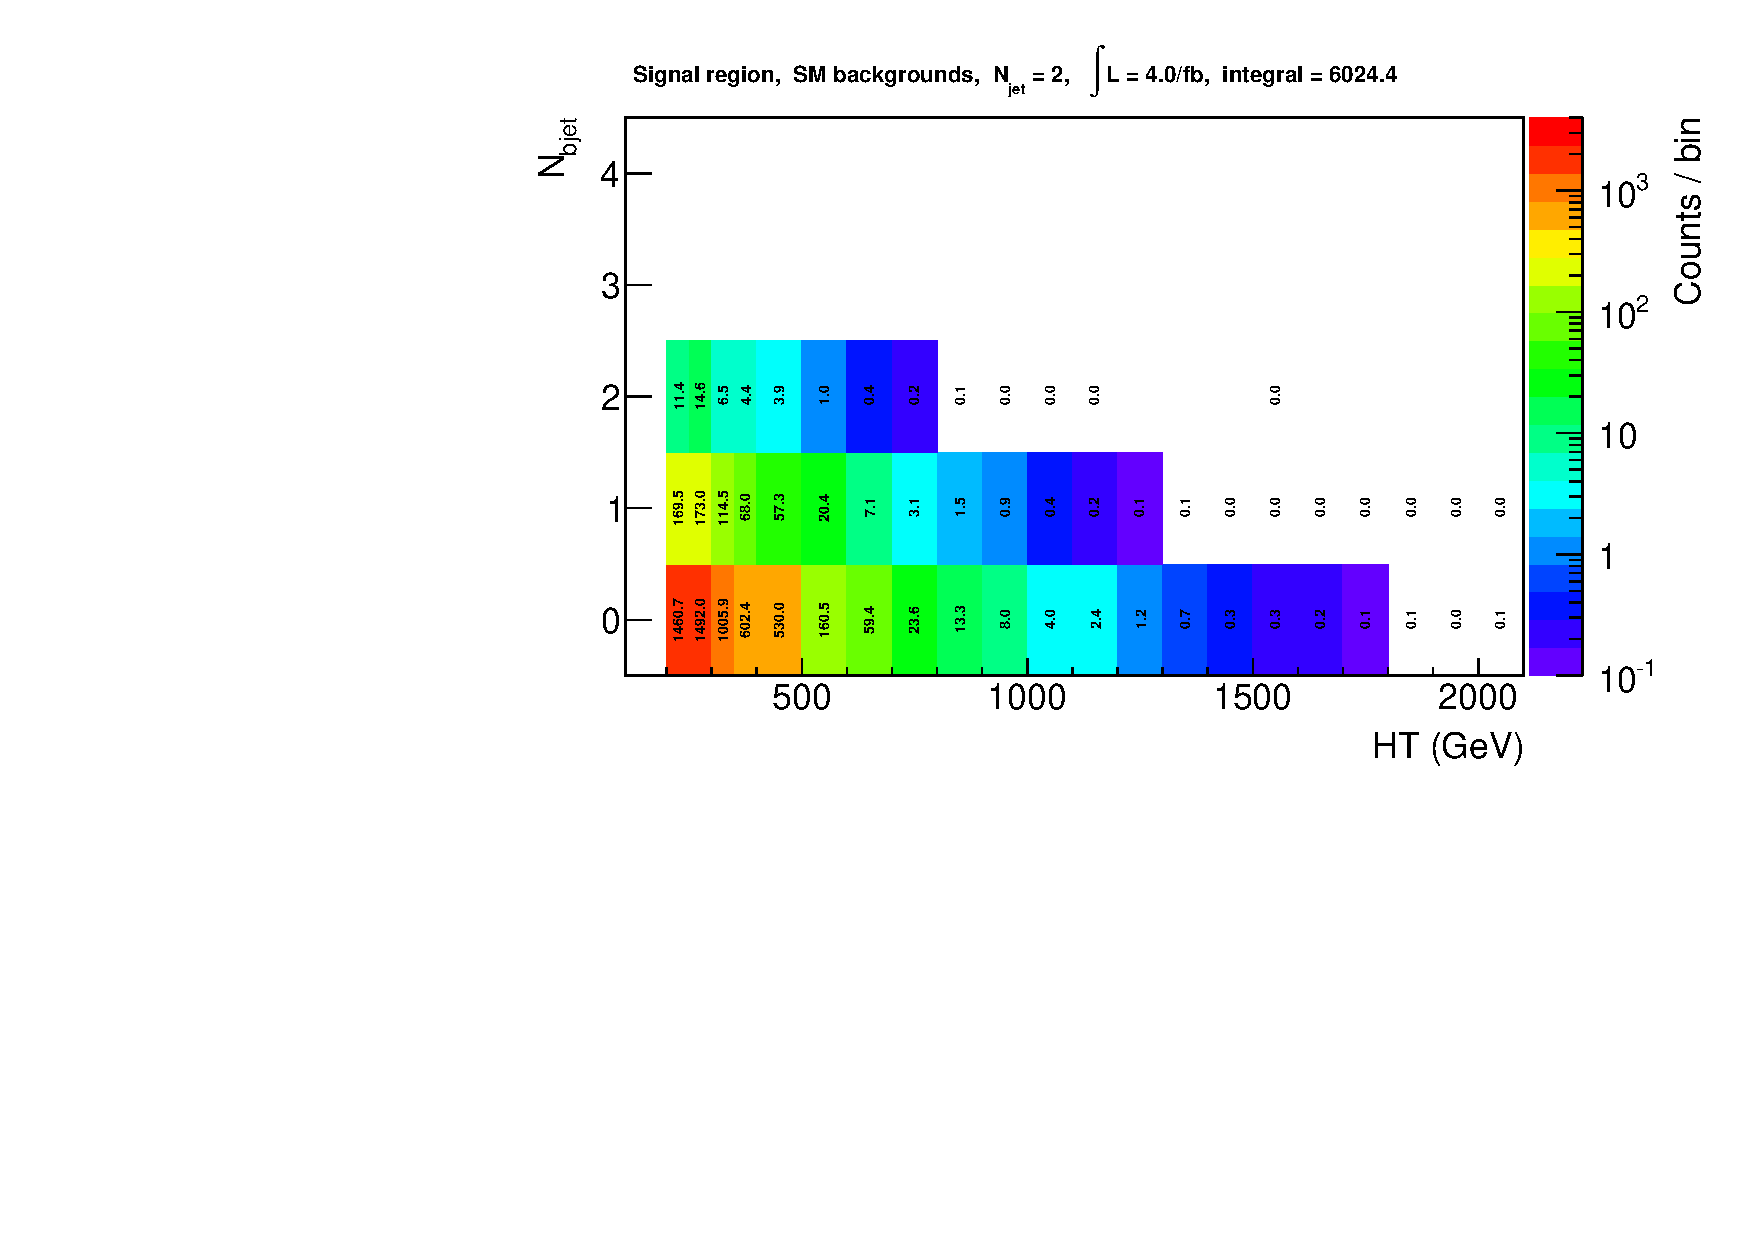
\includegraphics[width=0.5\textwidth]{figures/yieldPlots/had_ewk_eq2j.pdf}
  }~~
  \subfigure[Hadronic signal region yields for the \zinv background
  ($\njet = 2$)]{
    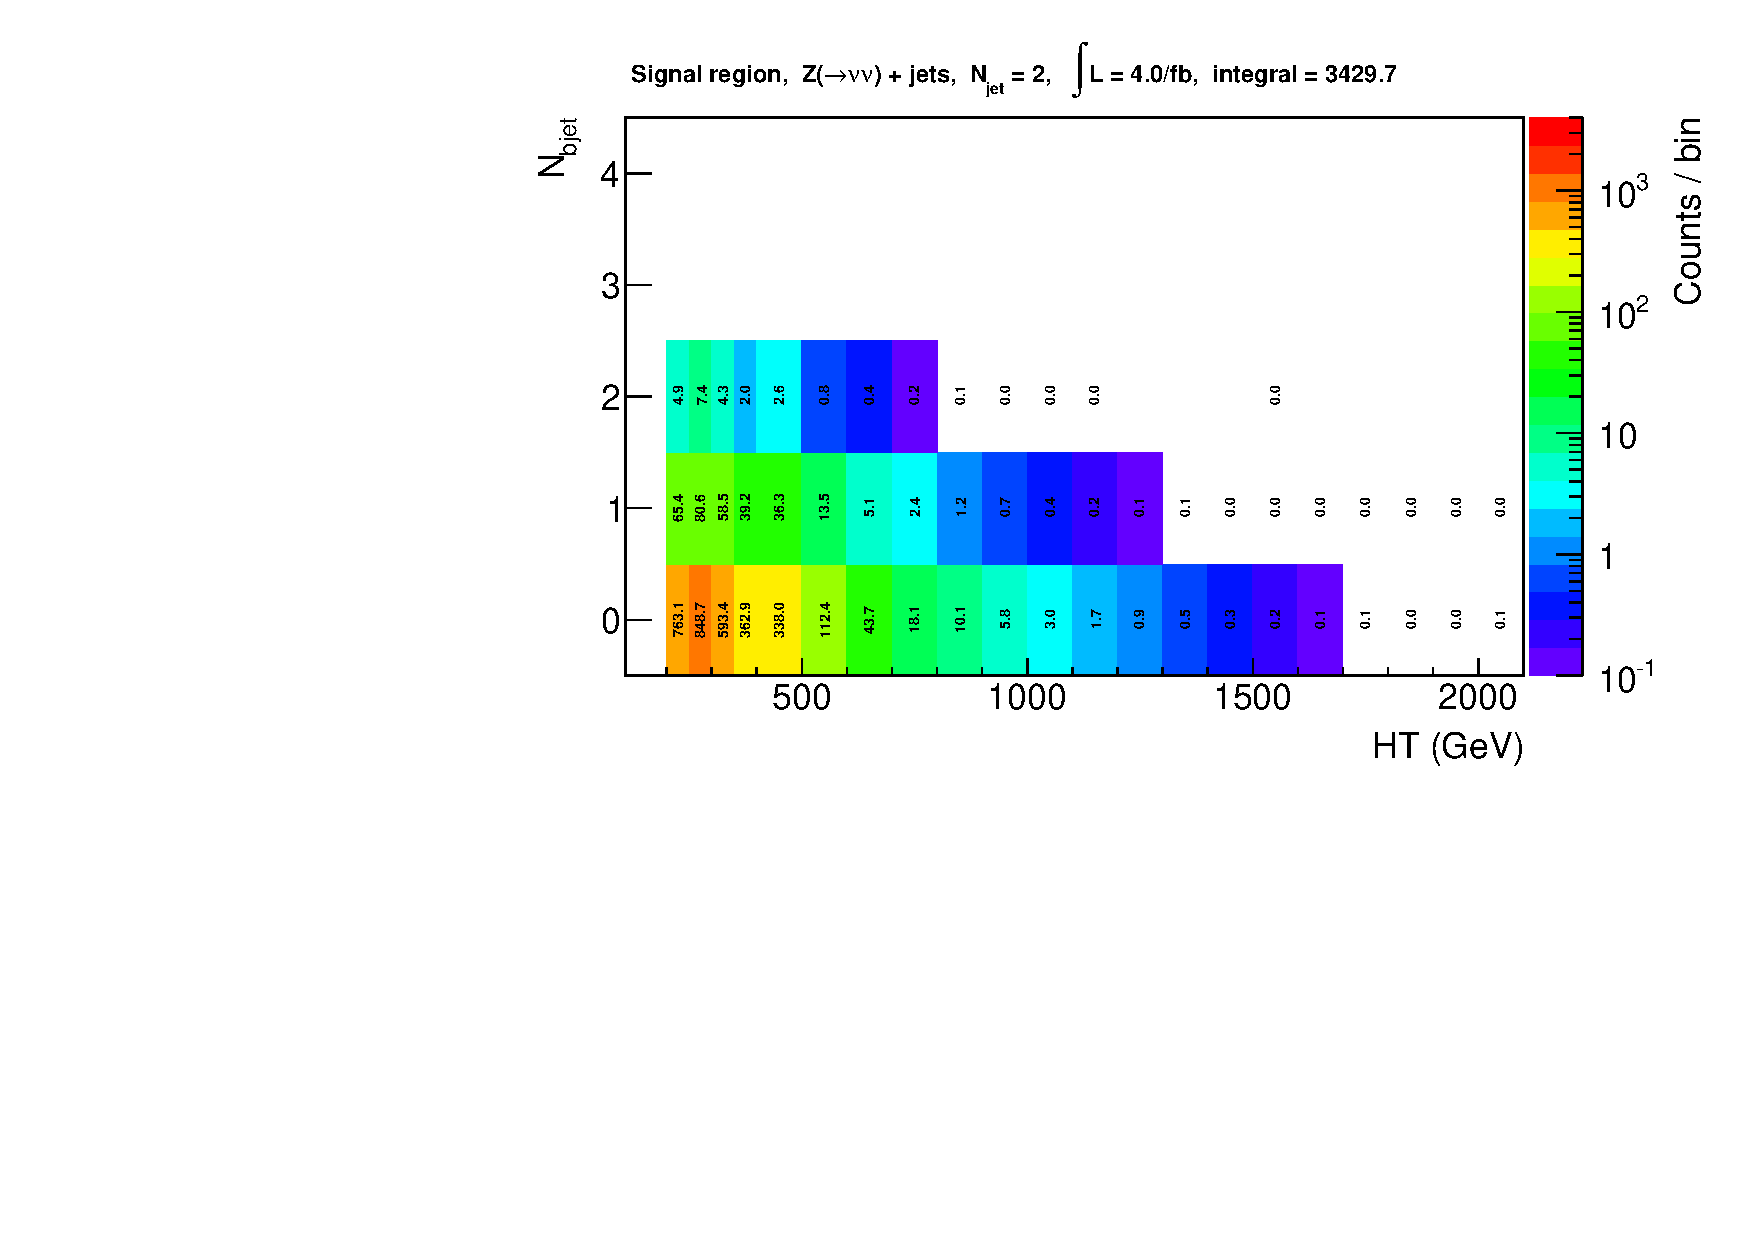
\includegraphics[width=0.5\textwidth]{figures/yieldPlots/had_zinv_eq2j.pdf}
  }\\
  \subfigure[Hadronic signal region yields for W~+~jets backtround
  ($\njet = 2$)]{
    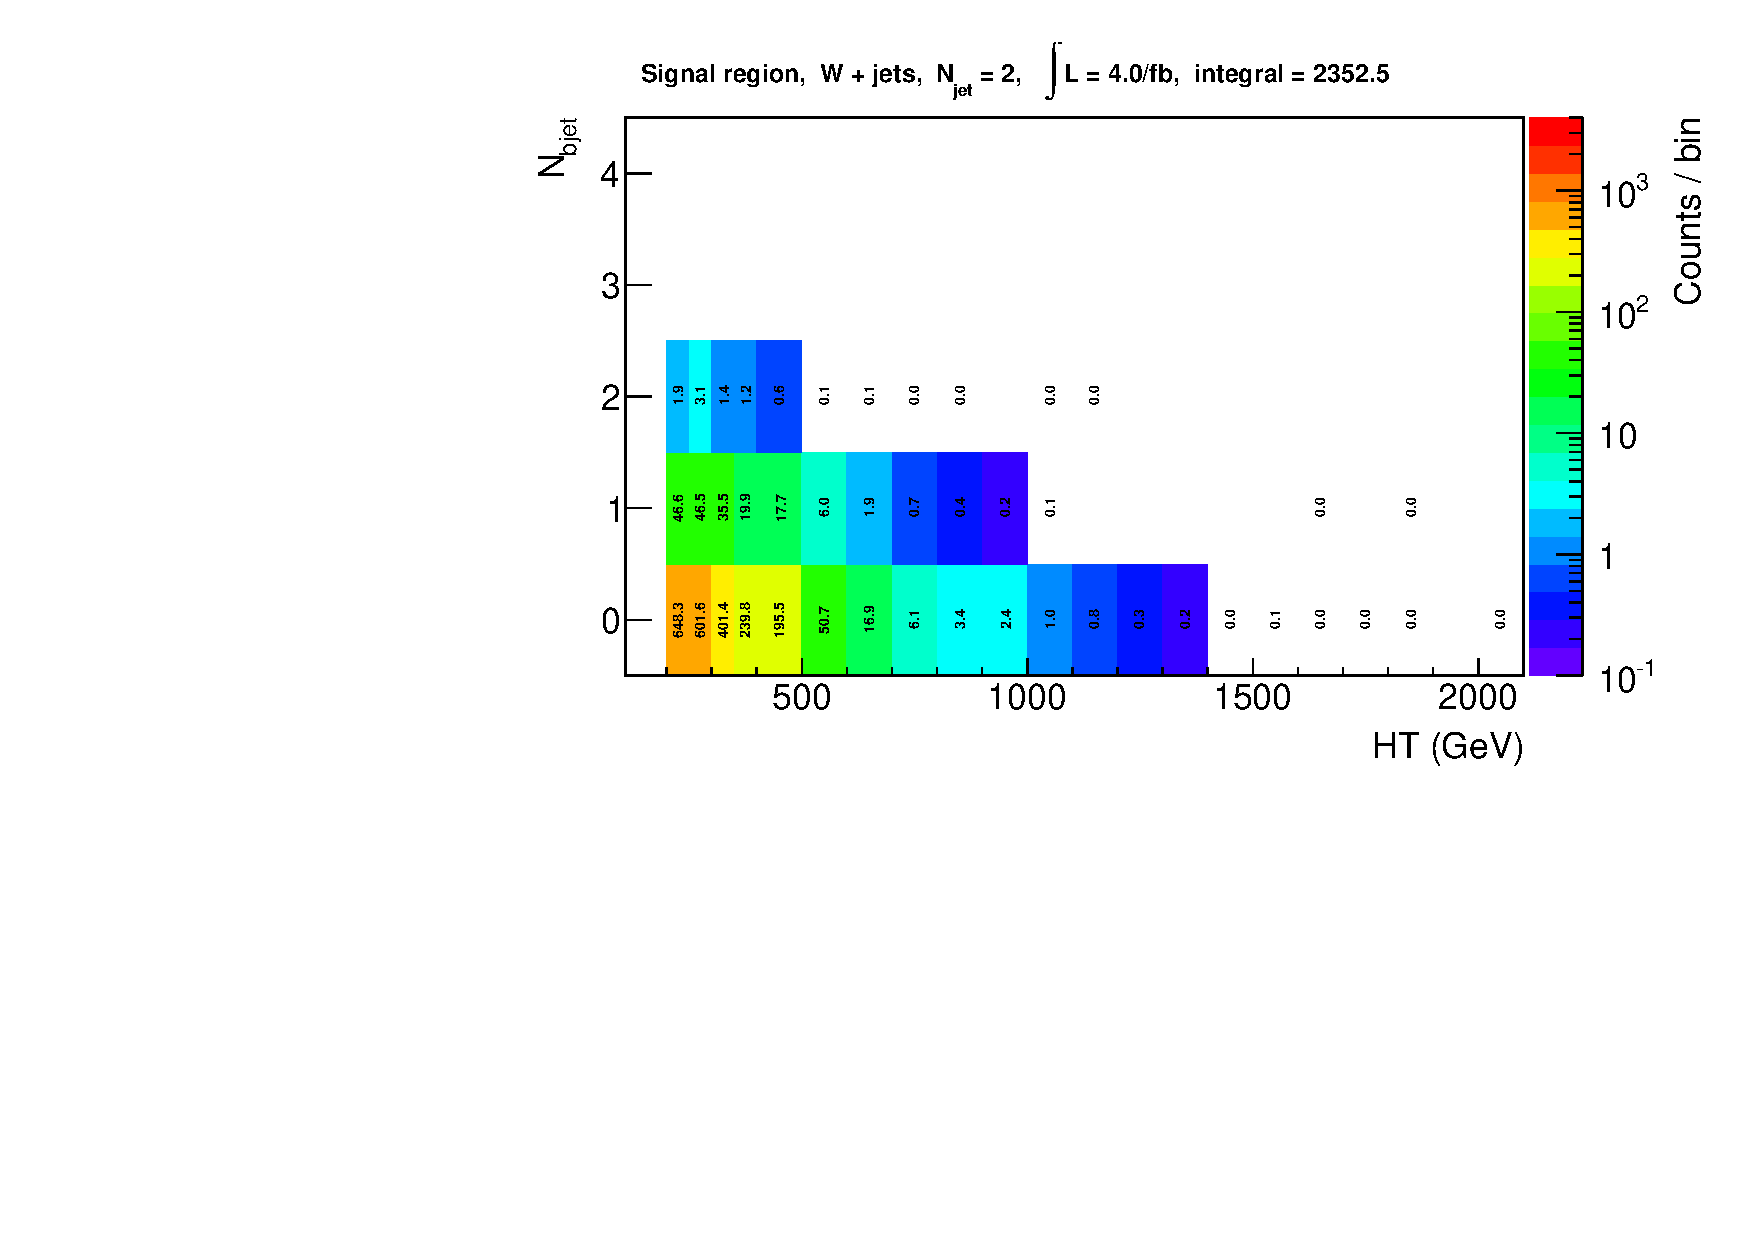
\includegraphics[width=0.5\textwidth]{figures/yieldPlots/had_wjets_eq2j.pdf}
  }~~
  \subfigure[Hadronic signal region yields for \ttbar background
  ($\njet = 2$)]{
    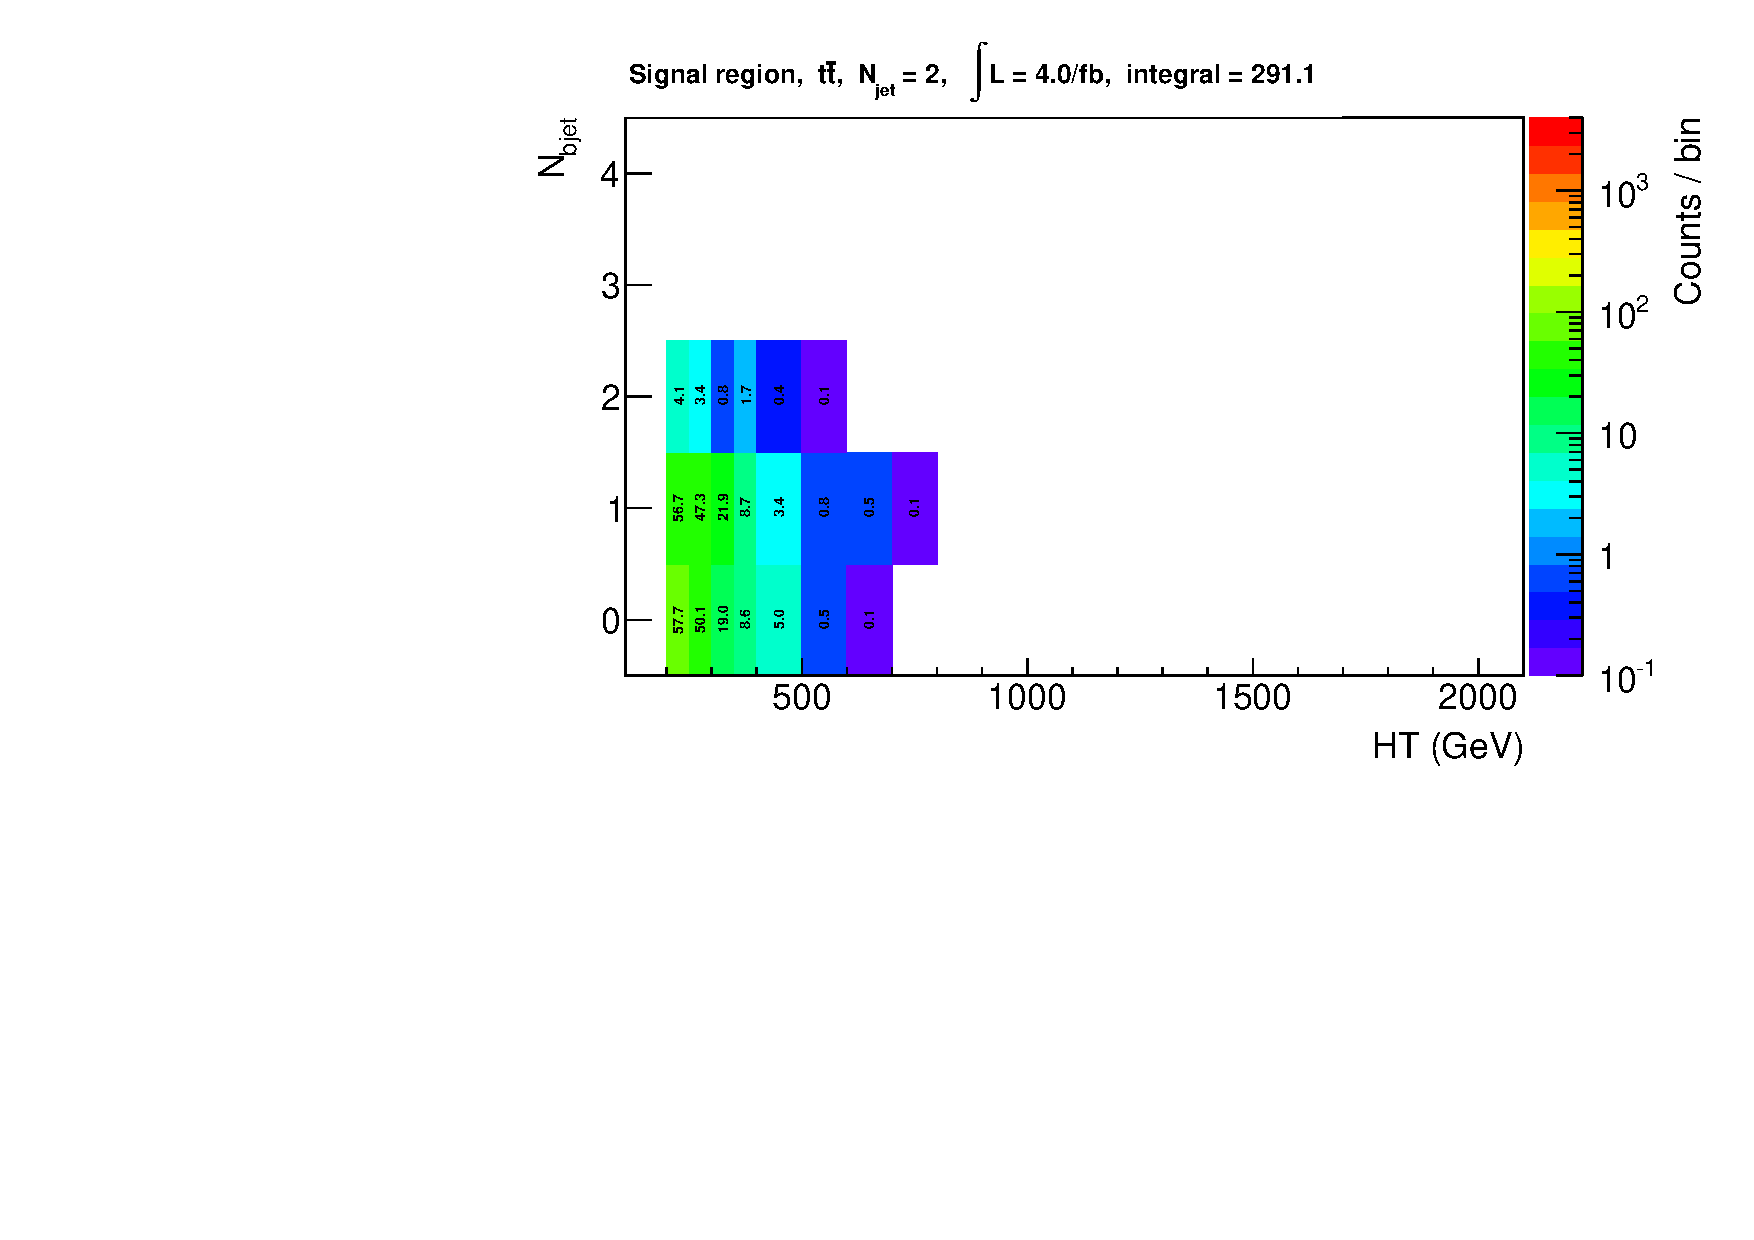
\includegraphics[width=0.5\textwidth]{figures/yieldPlots/had_ttbar_eq2j.pdf}
  }
  \\
  \subfigure[Hadronic signal region yields for electroweak backgrounds
  ($\njet = 3$)]{
    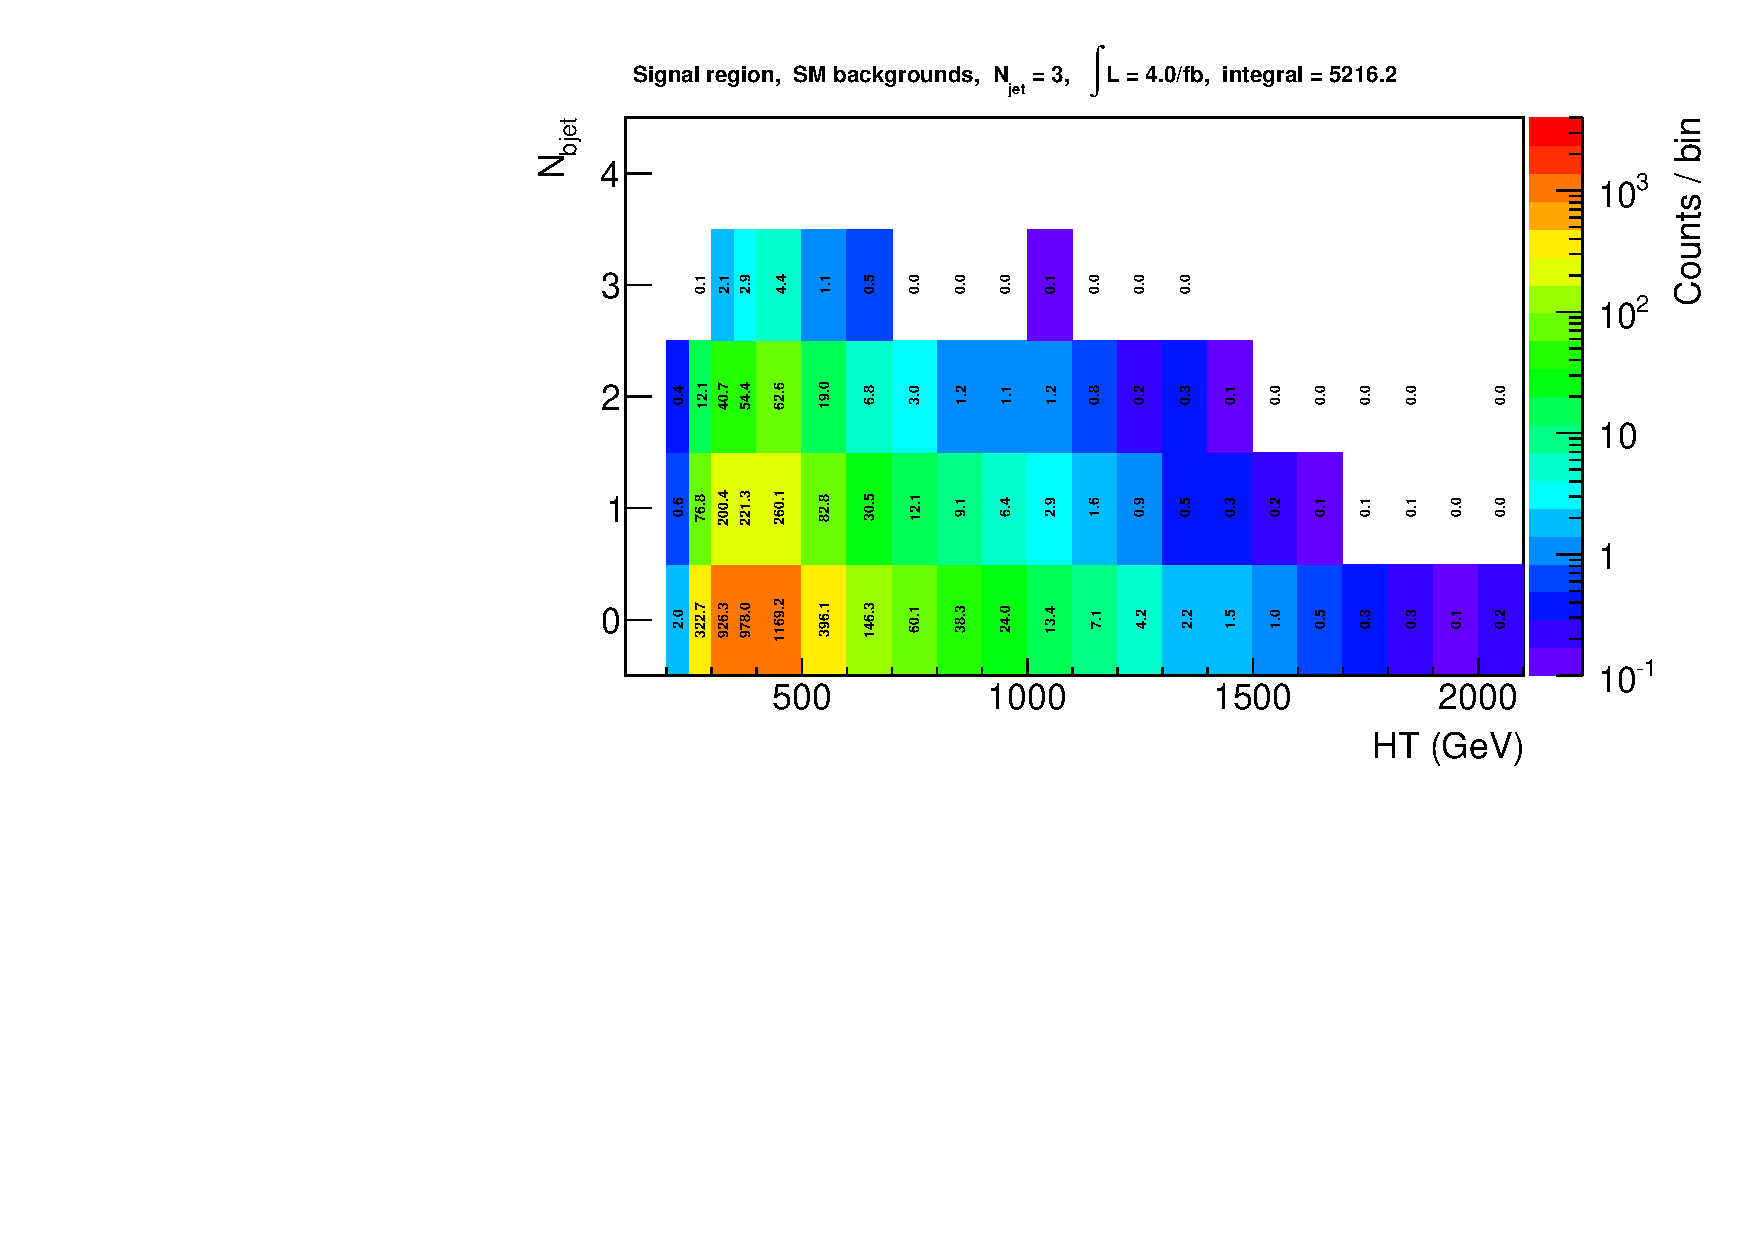
\includegraphics[width=0.5\textwidth]{figures/yieldPlots/had_ewk_eq3j.pdf}
  }~~
  \subfigure[Hadronic signal region yields for the \zinv background
  ($\njet = 3$)]{
    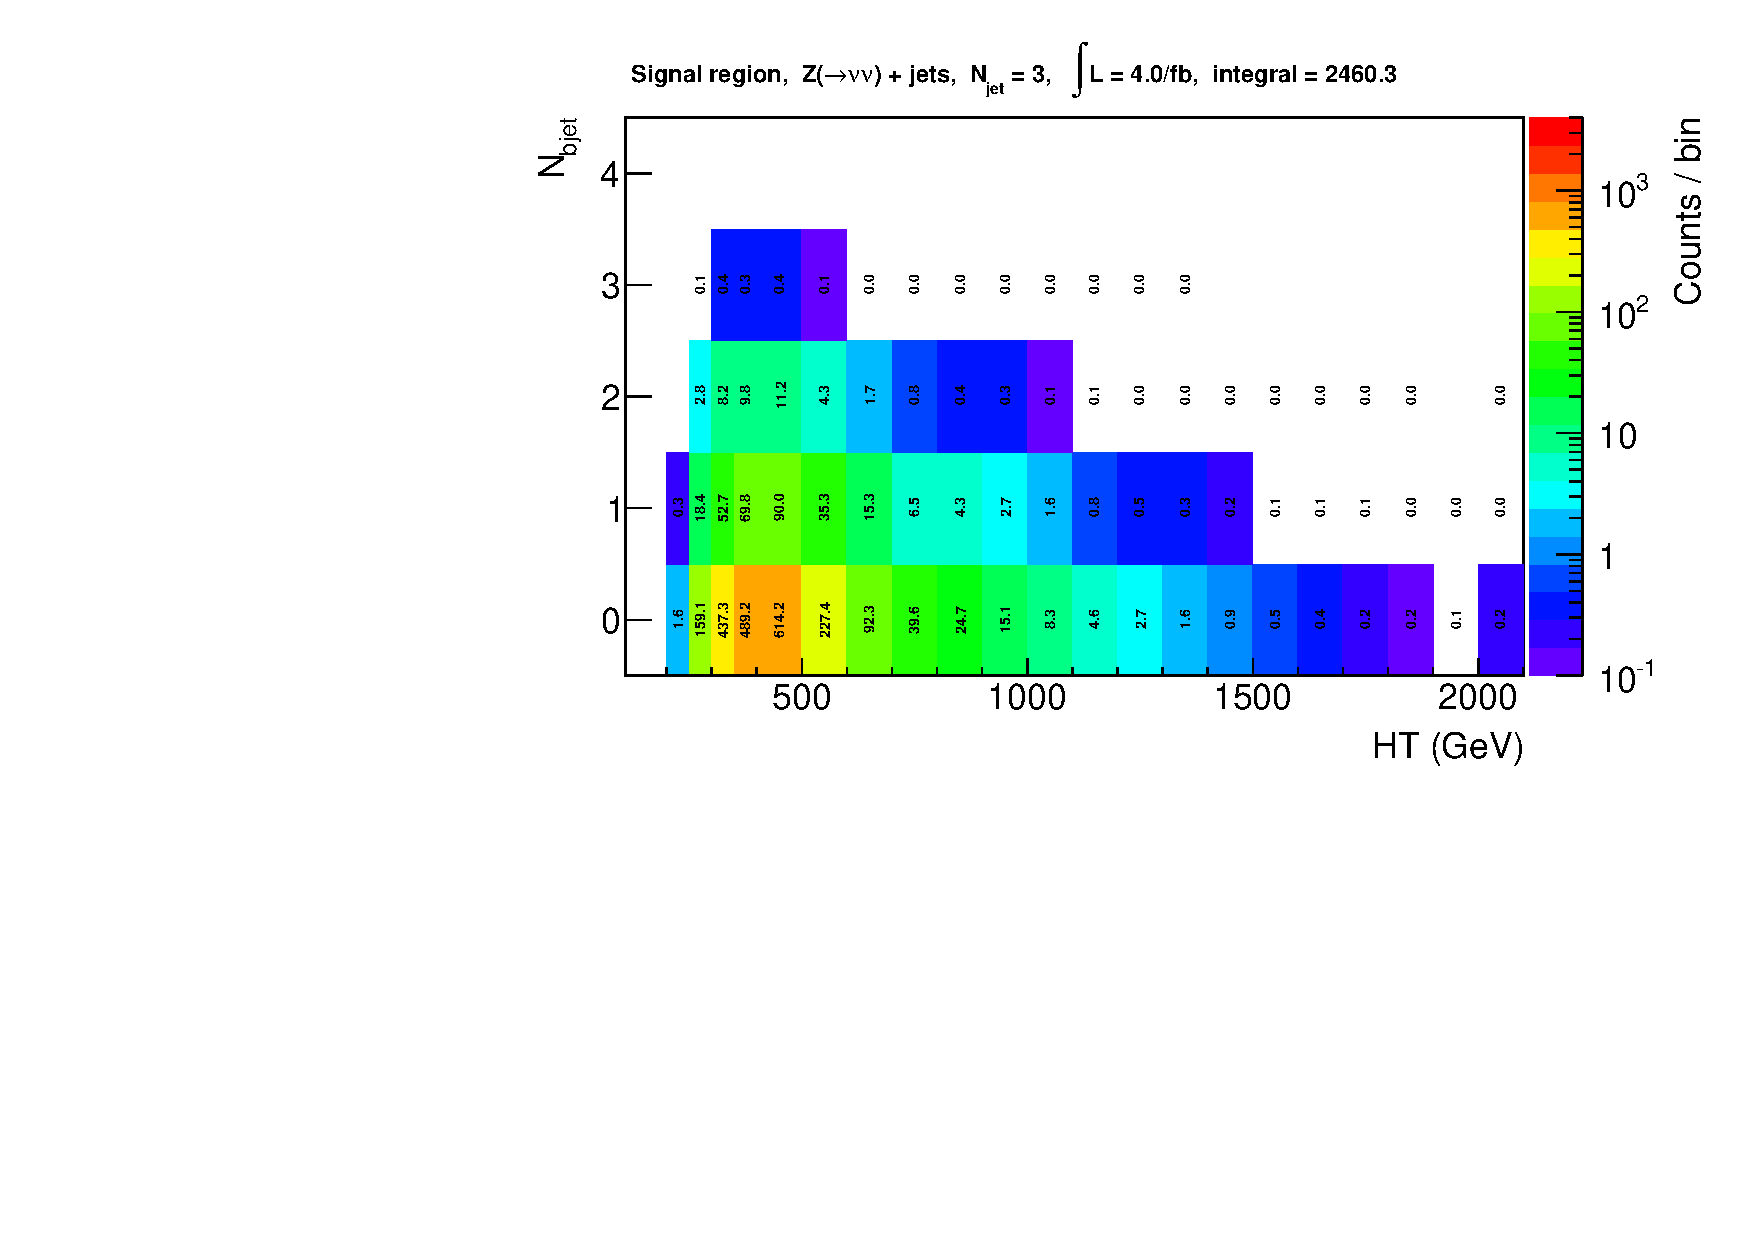
\includegraphics[width=0.5\textwidth]{figures/yieldPlots/had_zinv_eq3j.pdf}
  }\\
  \subfigure[Hadronic signal region yields for W~+~jets backtround
  ($\njet = 3$)]{
    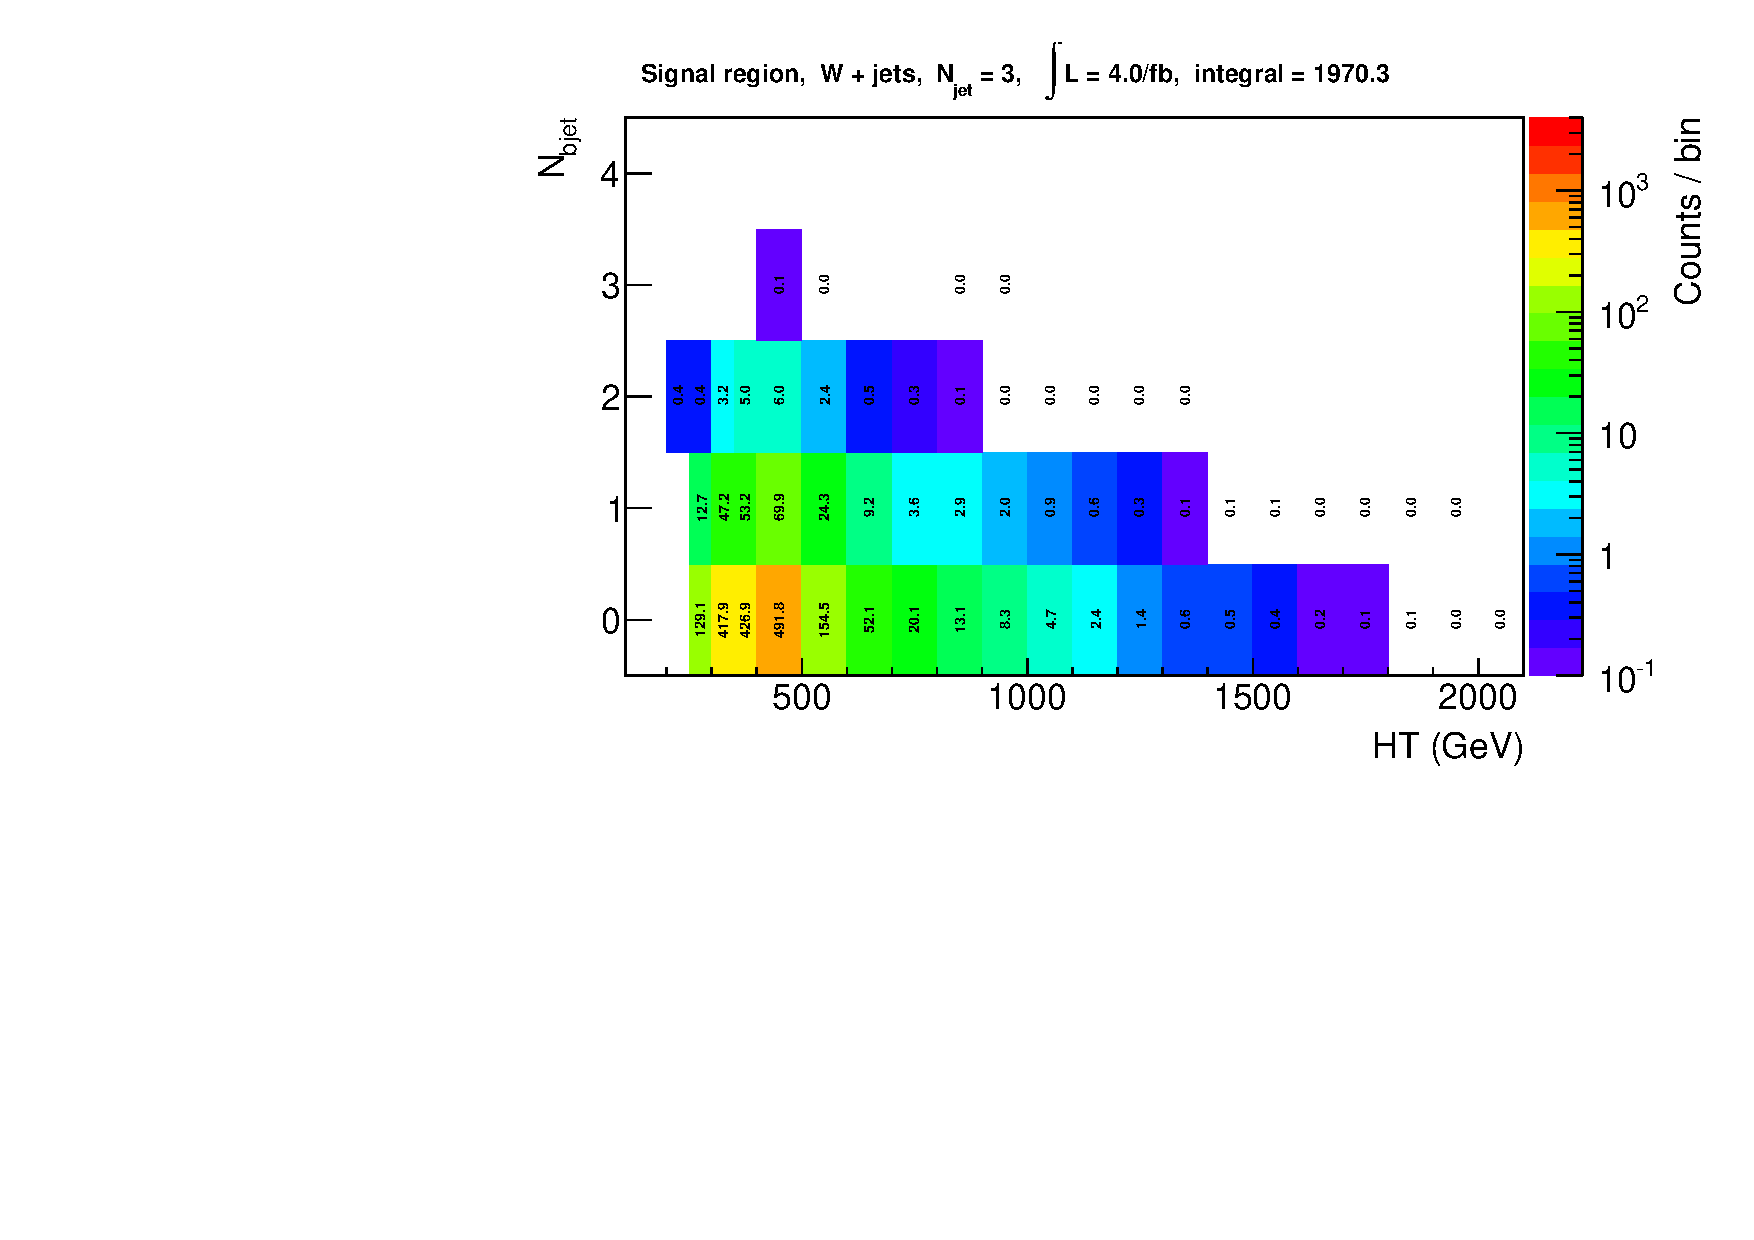
\includegraphics[width=0.5\textwidth]{figures/yieldPlots/had_wjets_eq3j.pdf}
  }~~
  \subfigure[Hadronic signal region yields for \ttbar background
  ($\njet = 3$)]{
    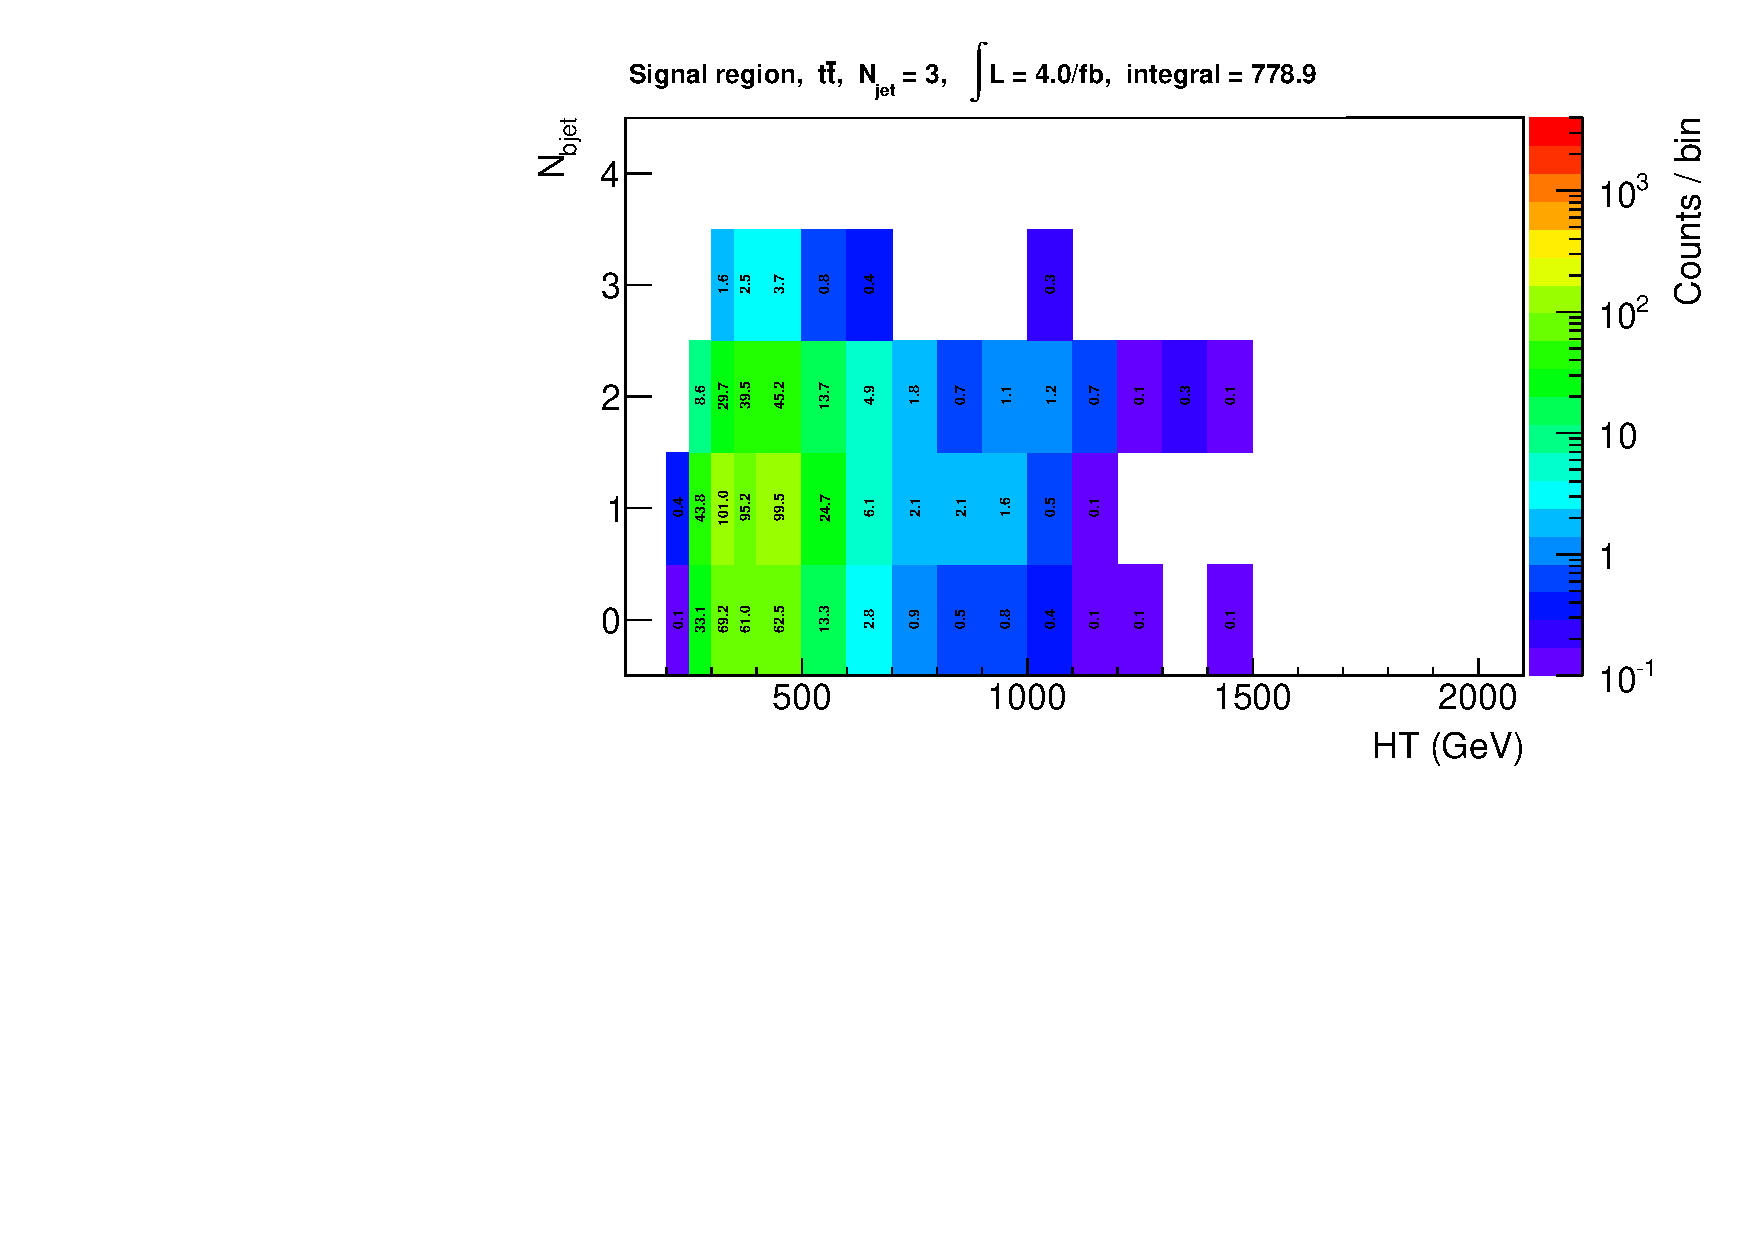
\includegraphics[width=0.5\textwidth]{figures/yieldPlots/had_ttbar_eq3j.pdf}
  }

  \\
  \subfigure[Hadronic signal region yields for electroweak backgrounds
  ($\njet = 4$)]{
    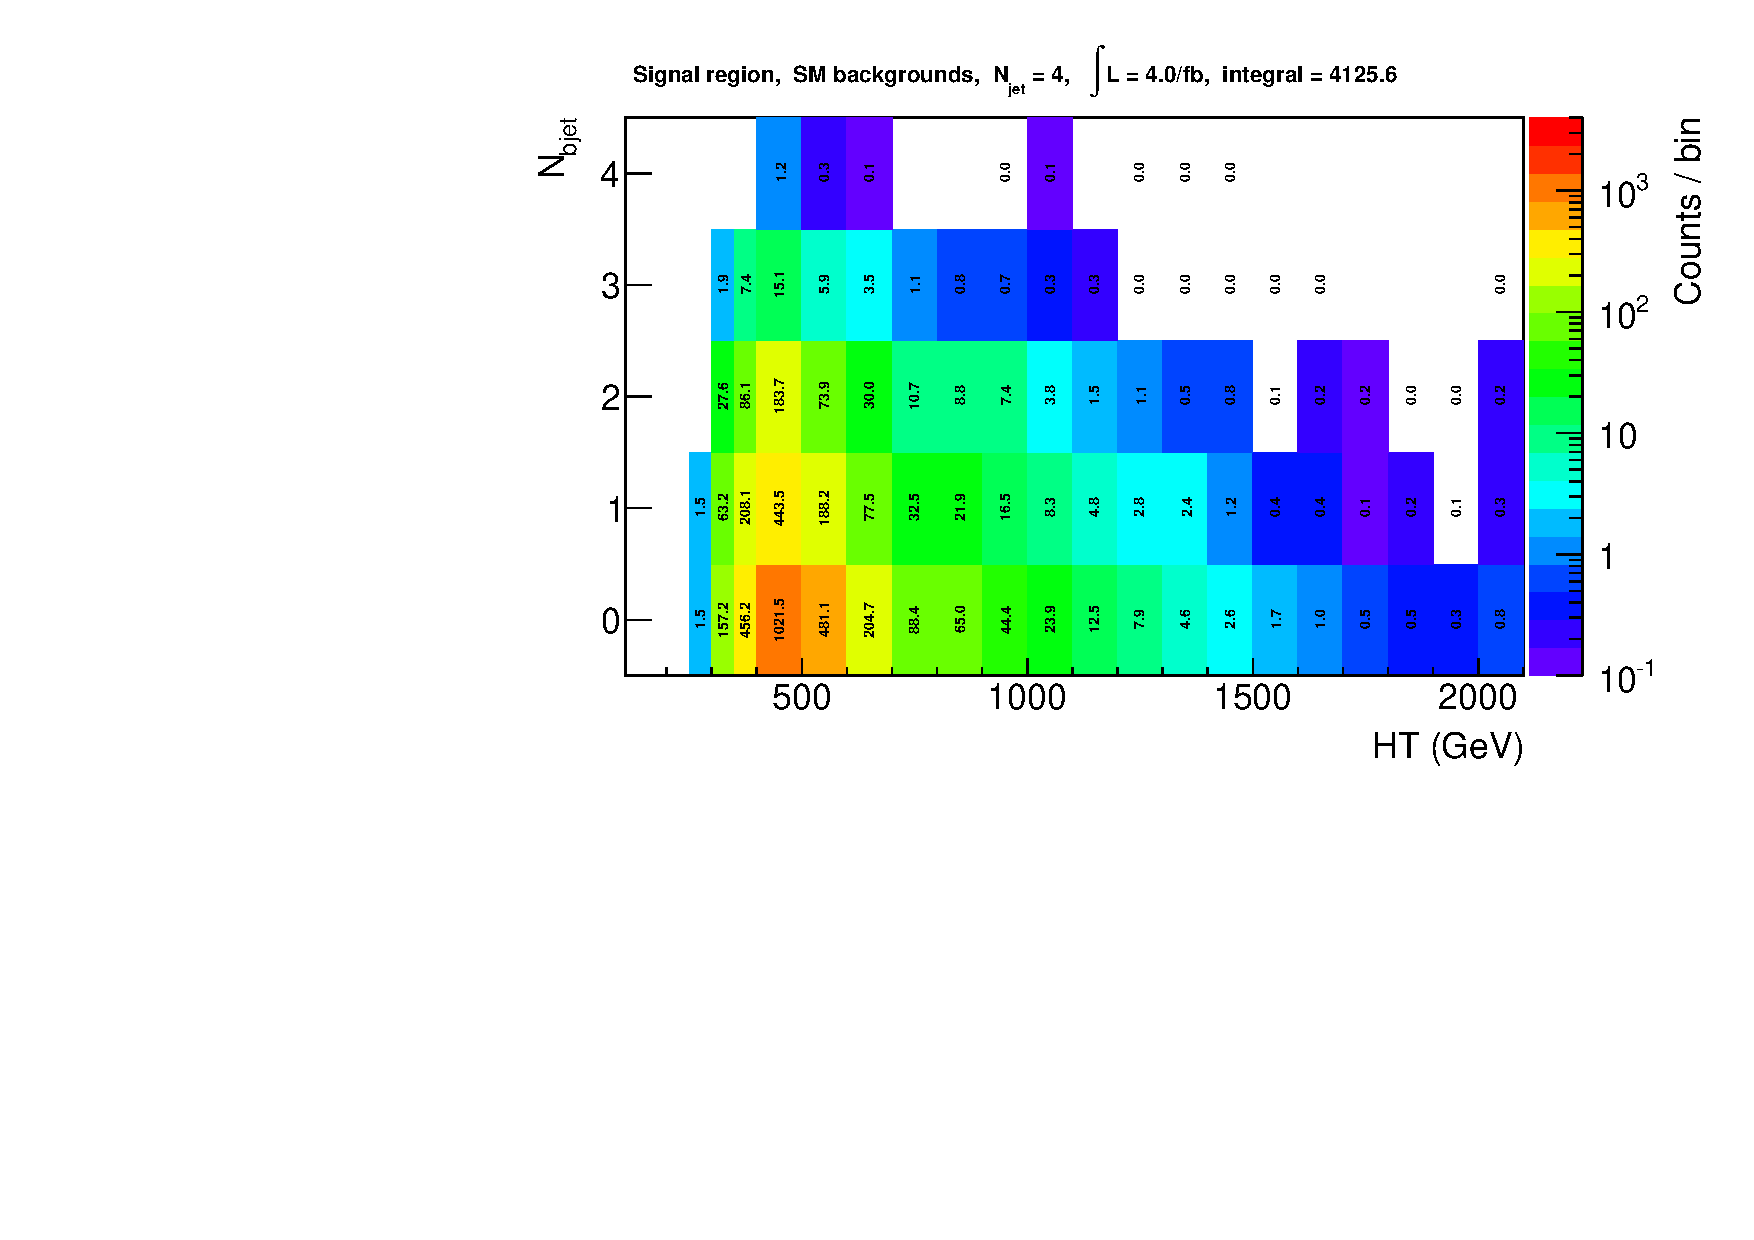
\includegraphics[width=0.5\textwidth]{figures/yieldPlots/had_ewk_eq4j.pdf}
  }~~
  \subfigure[Hadronic signal region yields for the \zinv background
  ($\njet = 4$)]{
    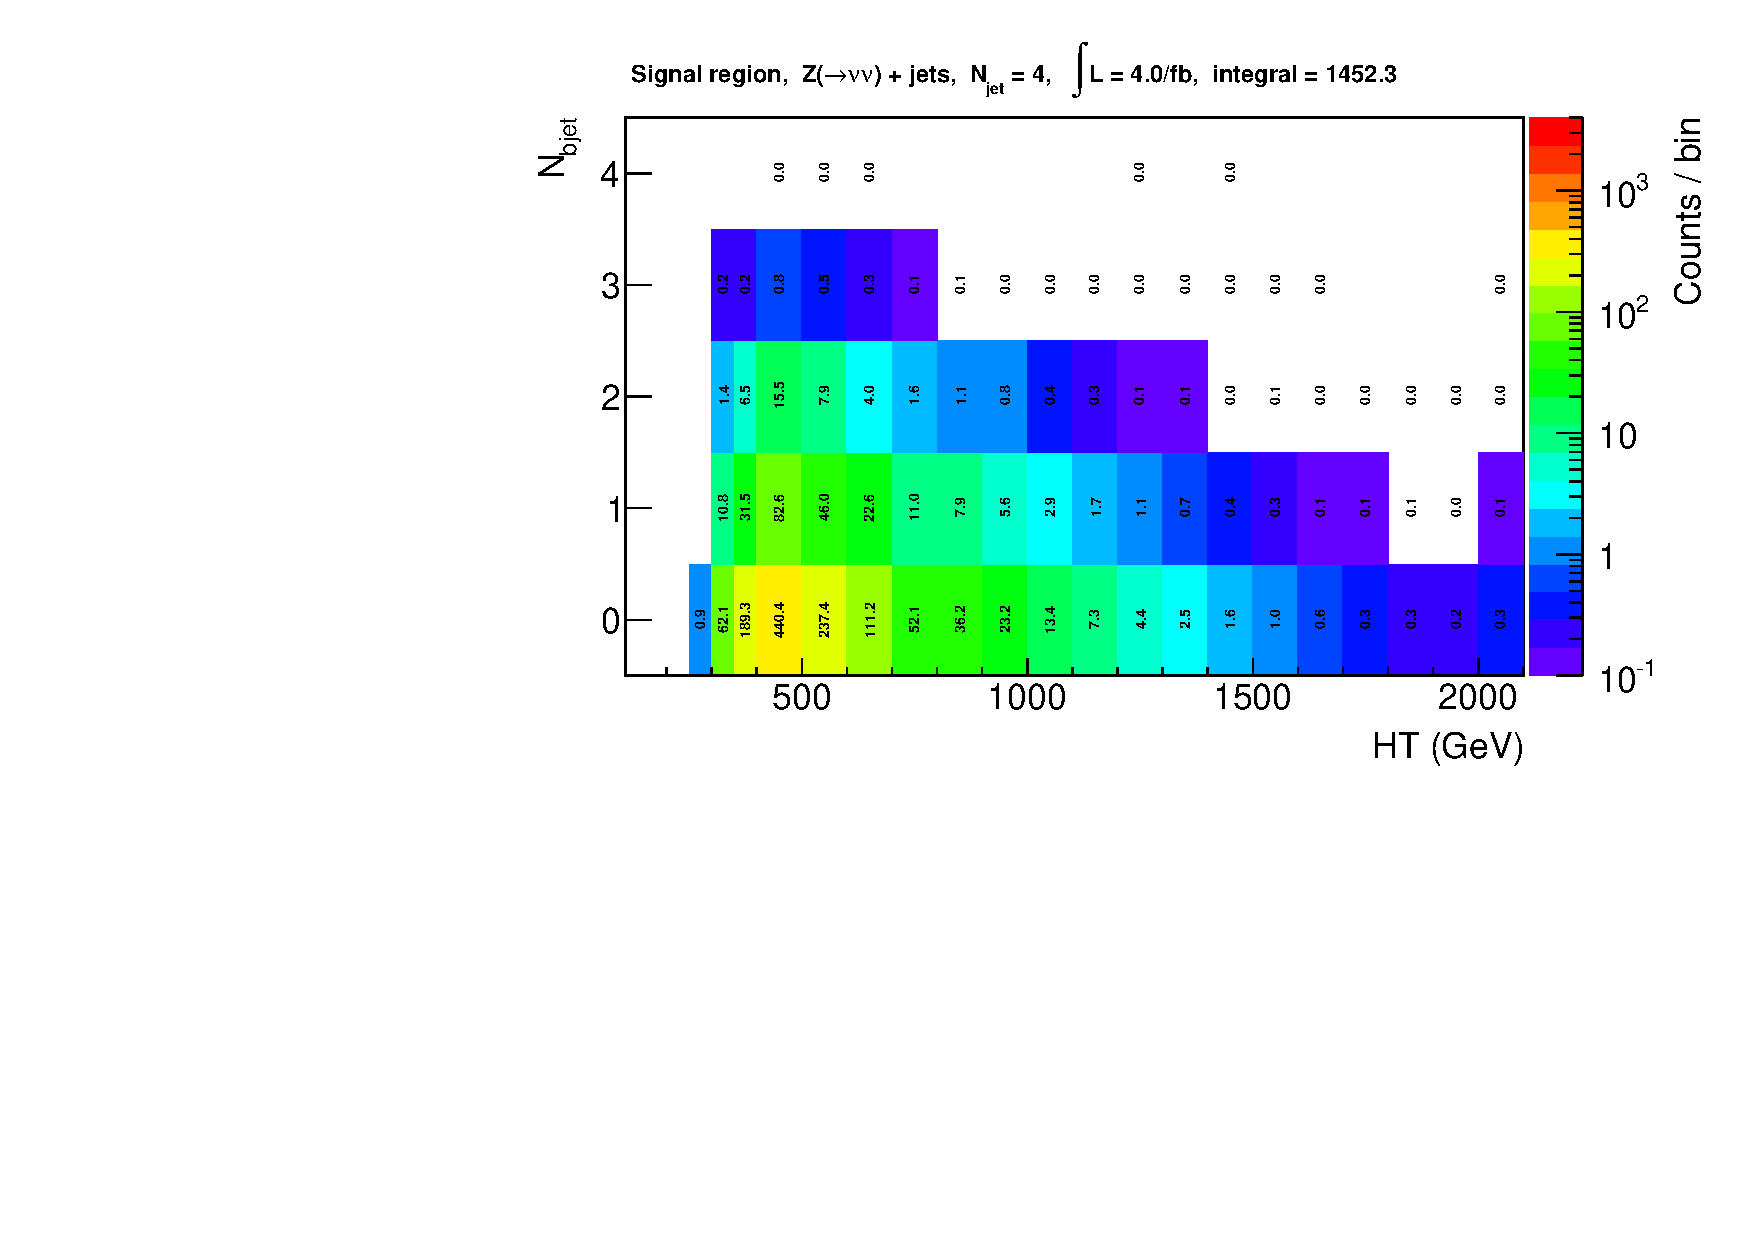
\includegraphics[width=0.5\textwidth]{figures/yieldPlots/had_zinv_eq4j.pdf}
  }\\
  \subfigure[Hadronic signal region yields for W~+~jets backtround
  ($\njet = 4$)]{
    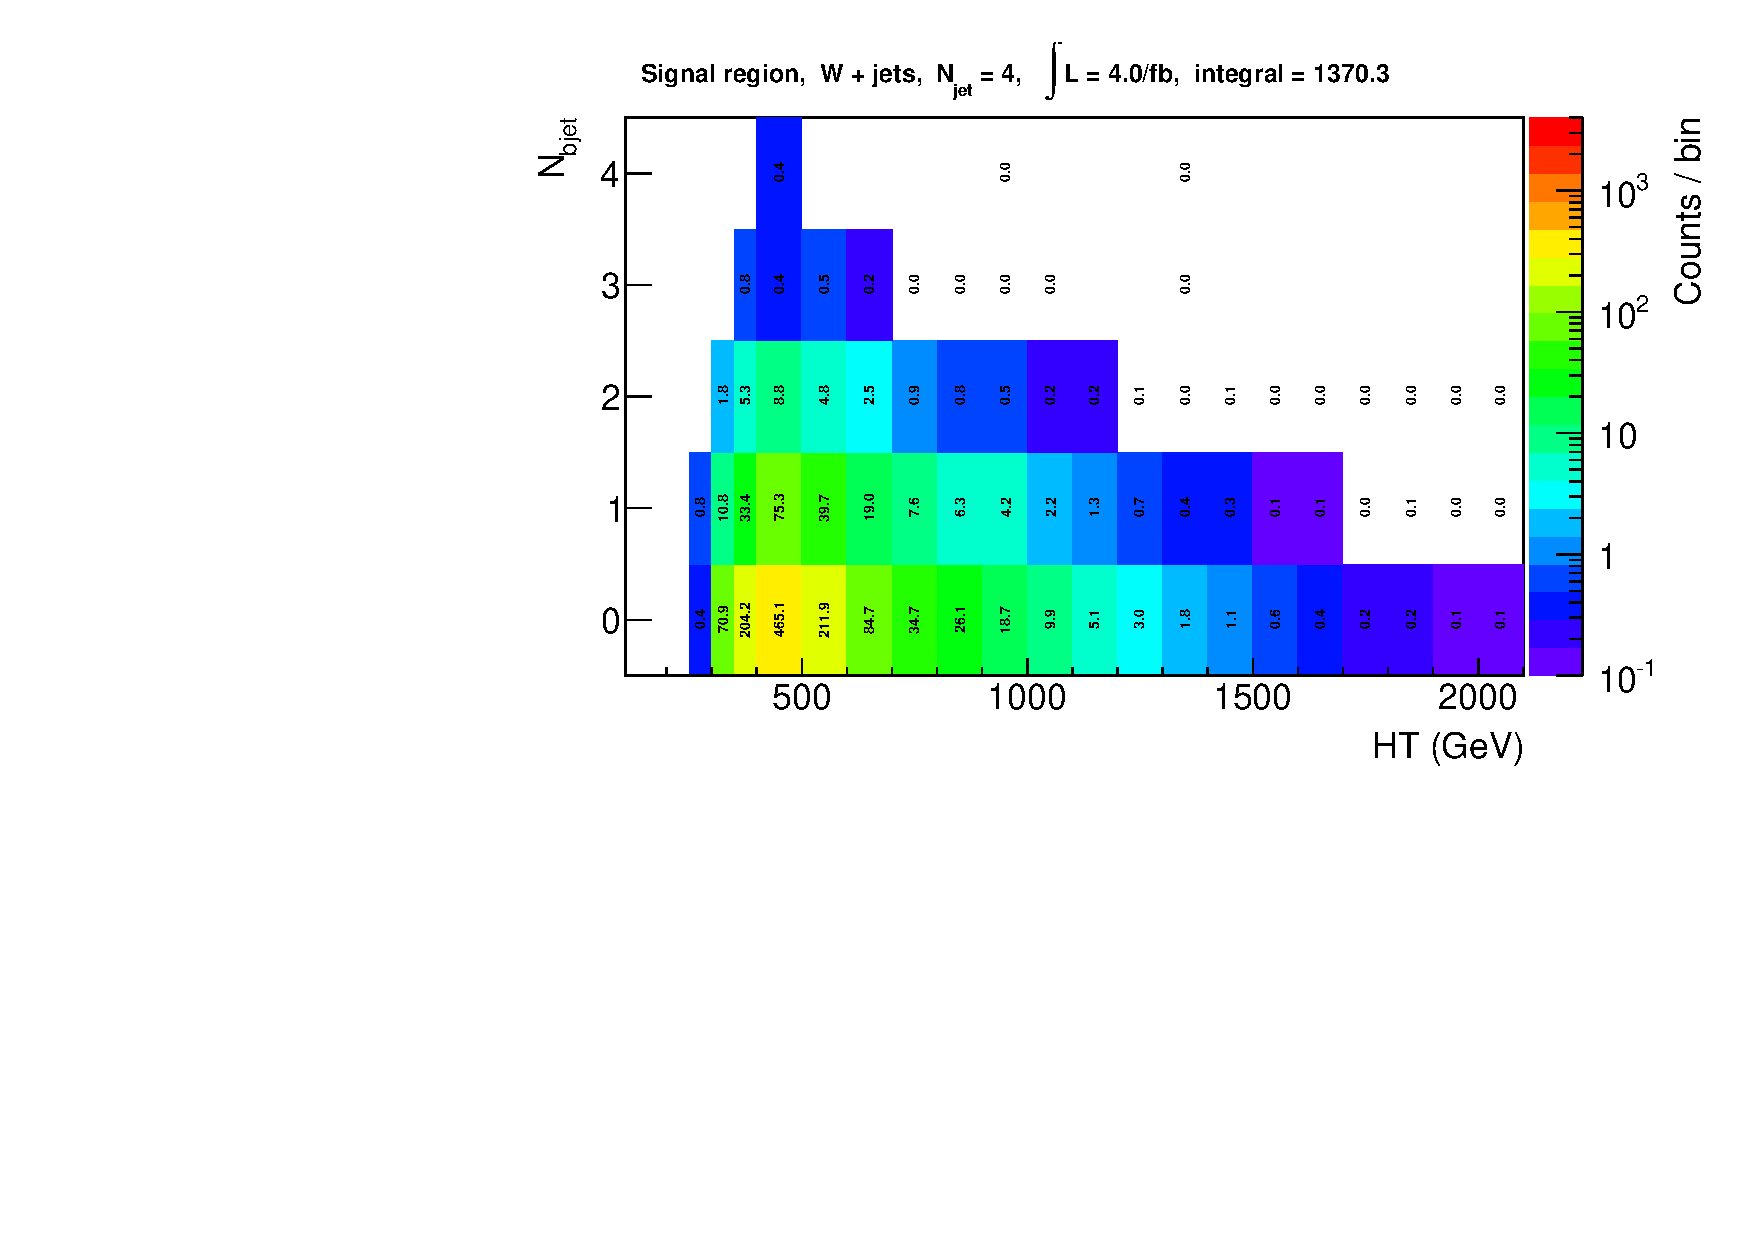
\includegraphics[width=0.5\textwidth]{figures/yieldPlots/had_wjets_eq4j.pdf}
  }~~
  \subfigure[Hadronic signal region yields for \ttbar background
  ($\njet = 4$)]{
    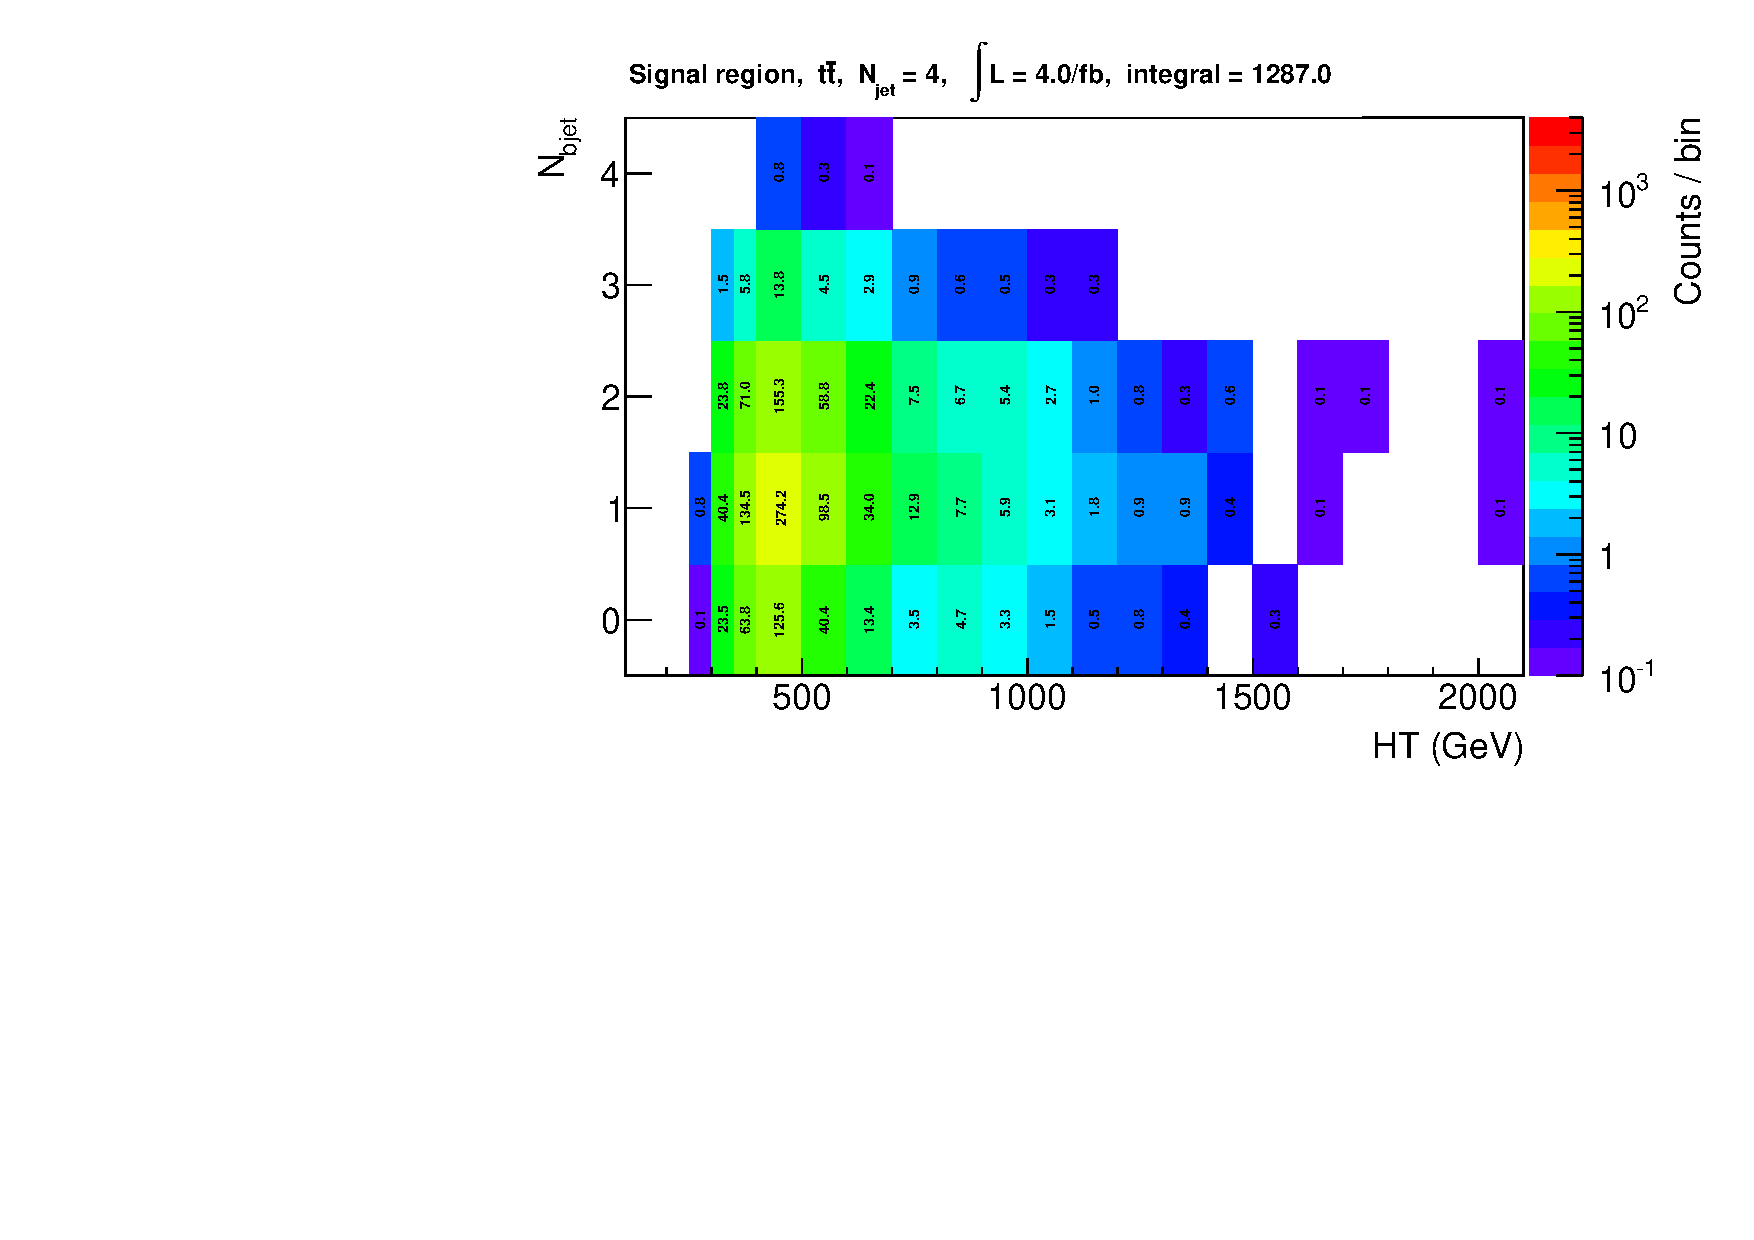
\includegraphics[width=0.5\textwidth]{figures/yieldPlots/had_ttbar_eq4j.pdf}
  }

  \\
  \subfigure[Hadronic signal region yields for electroweak backgrounds
  ($\njet \geq 5$)]{
    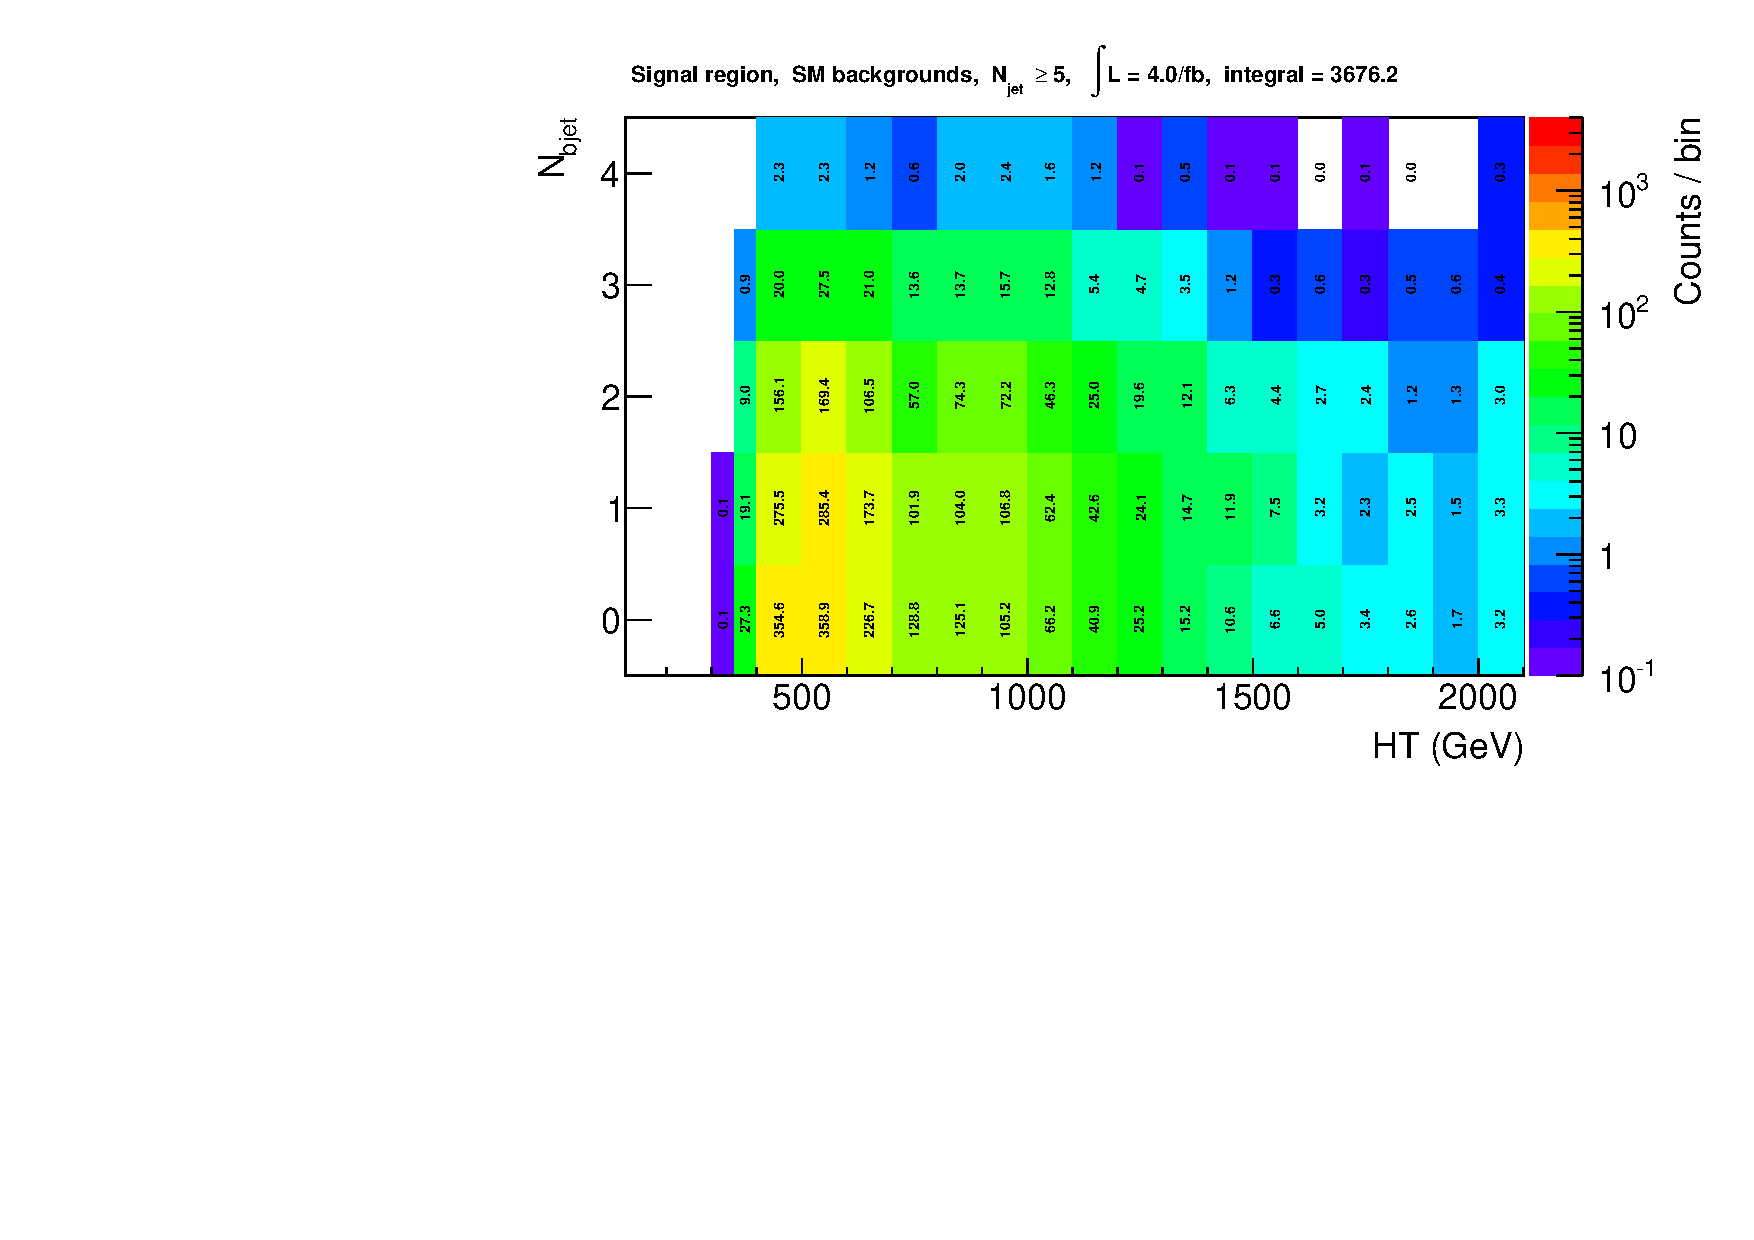
\includegraphics[width=0.5\textwidth]{figures/yieldPlots/had_ewk_ge5j.pdf}
  } ~~
  \subfigure[Hadronic signal region yields for the \zinv background
  ($\njet \geq 5$)]{
    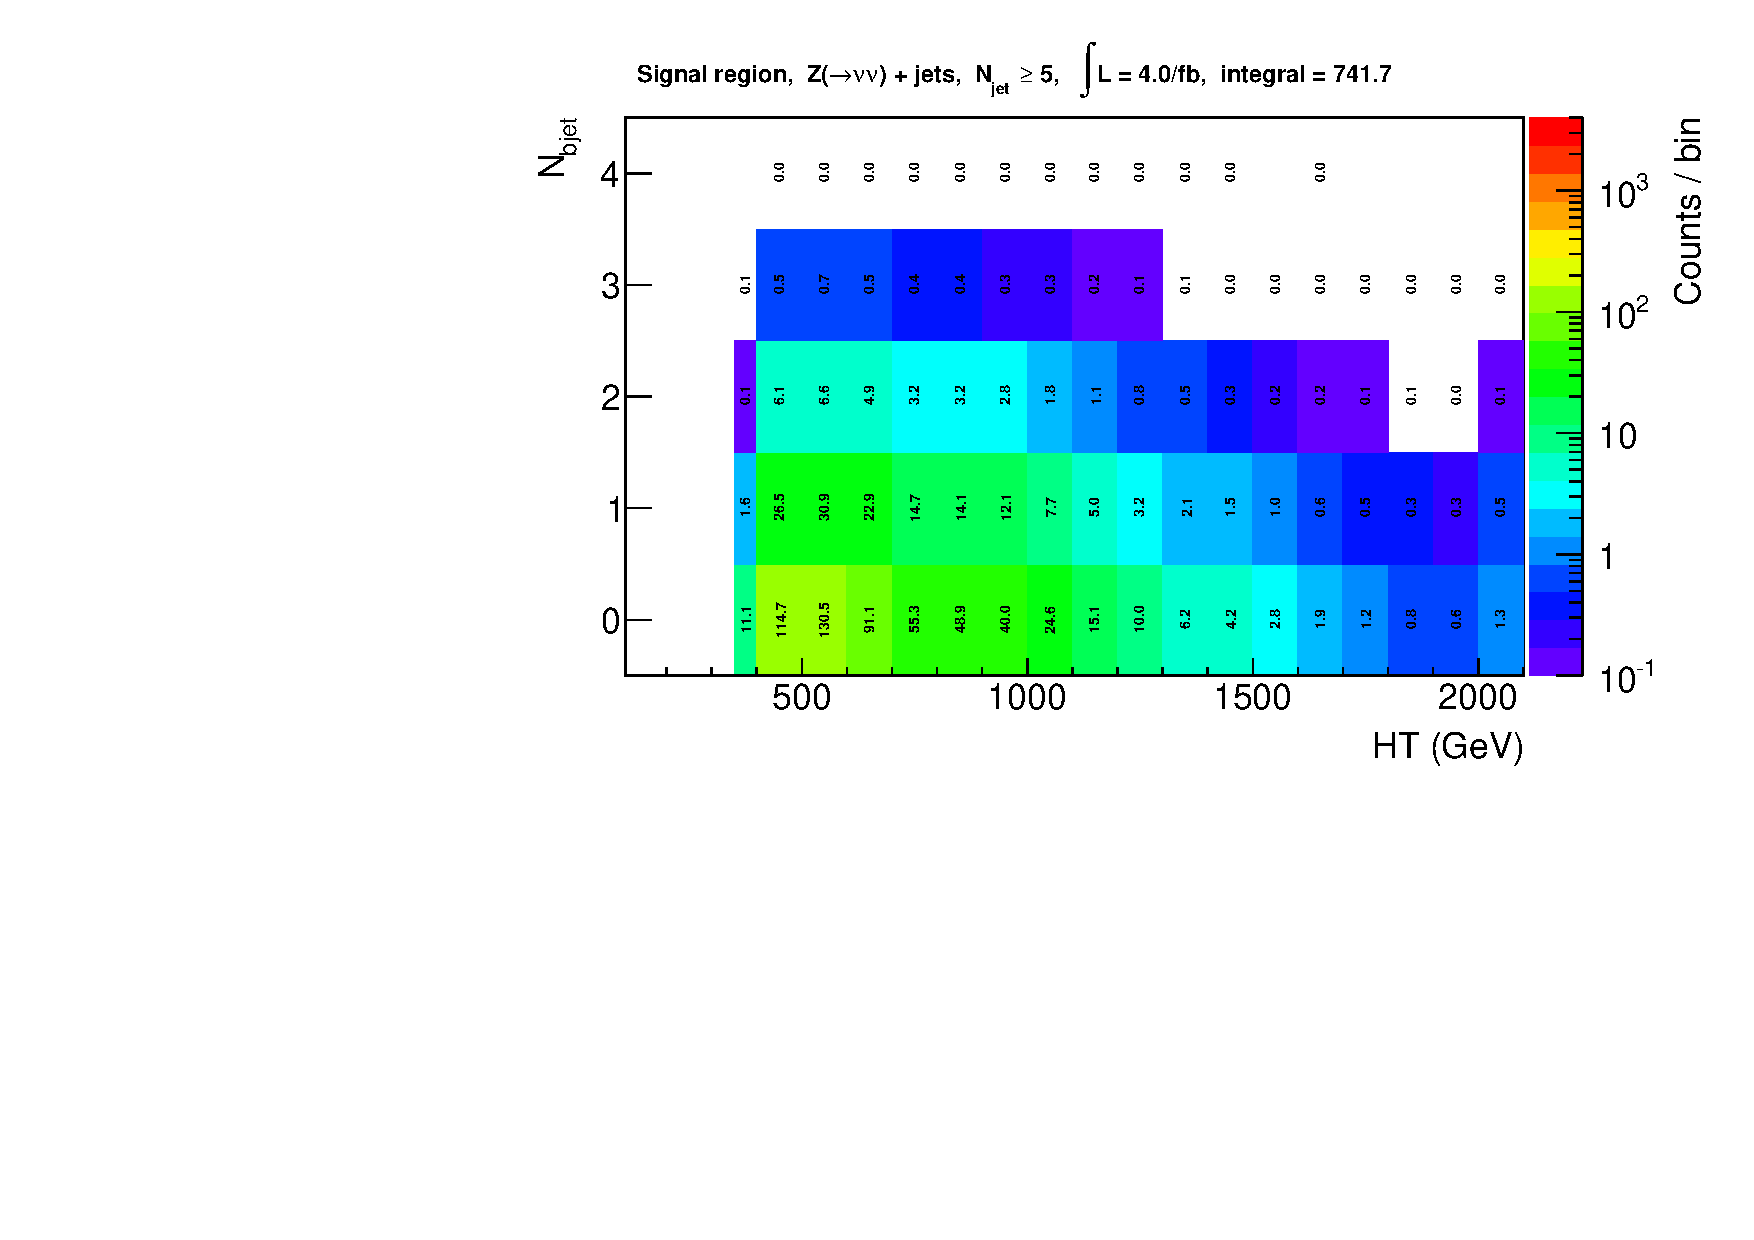
\includegraphics[width=0.5\textwidth]{figures/yieldPlots/had_zinv_ge5j.pdf}
  }\\
  \subfigure[Hadronic signal region yields for W~+~jets backtround
  ($\njet \geq 5$)]{
    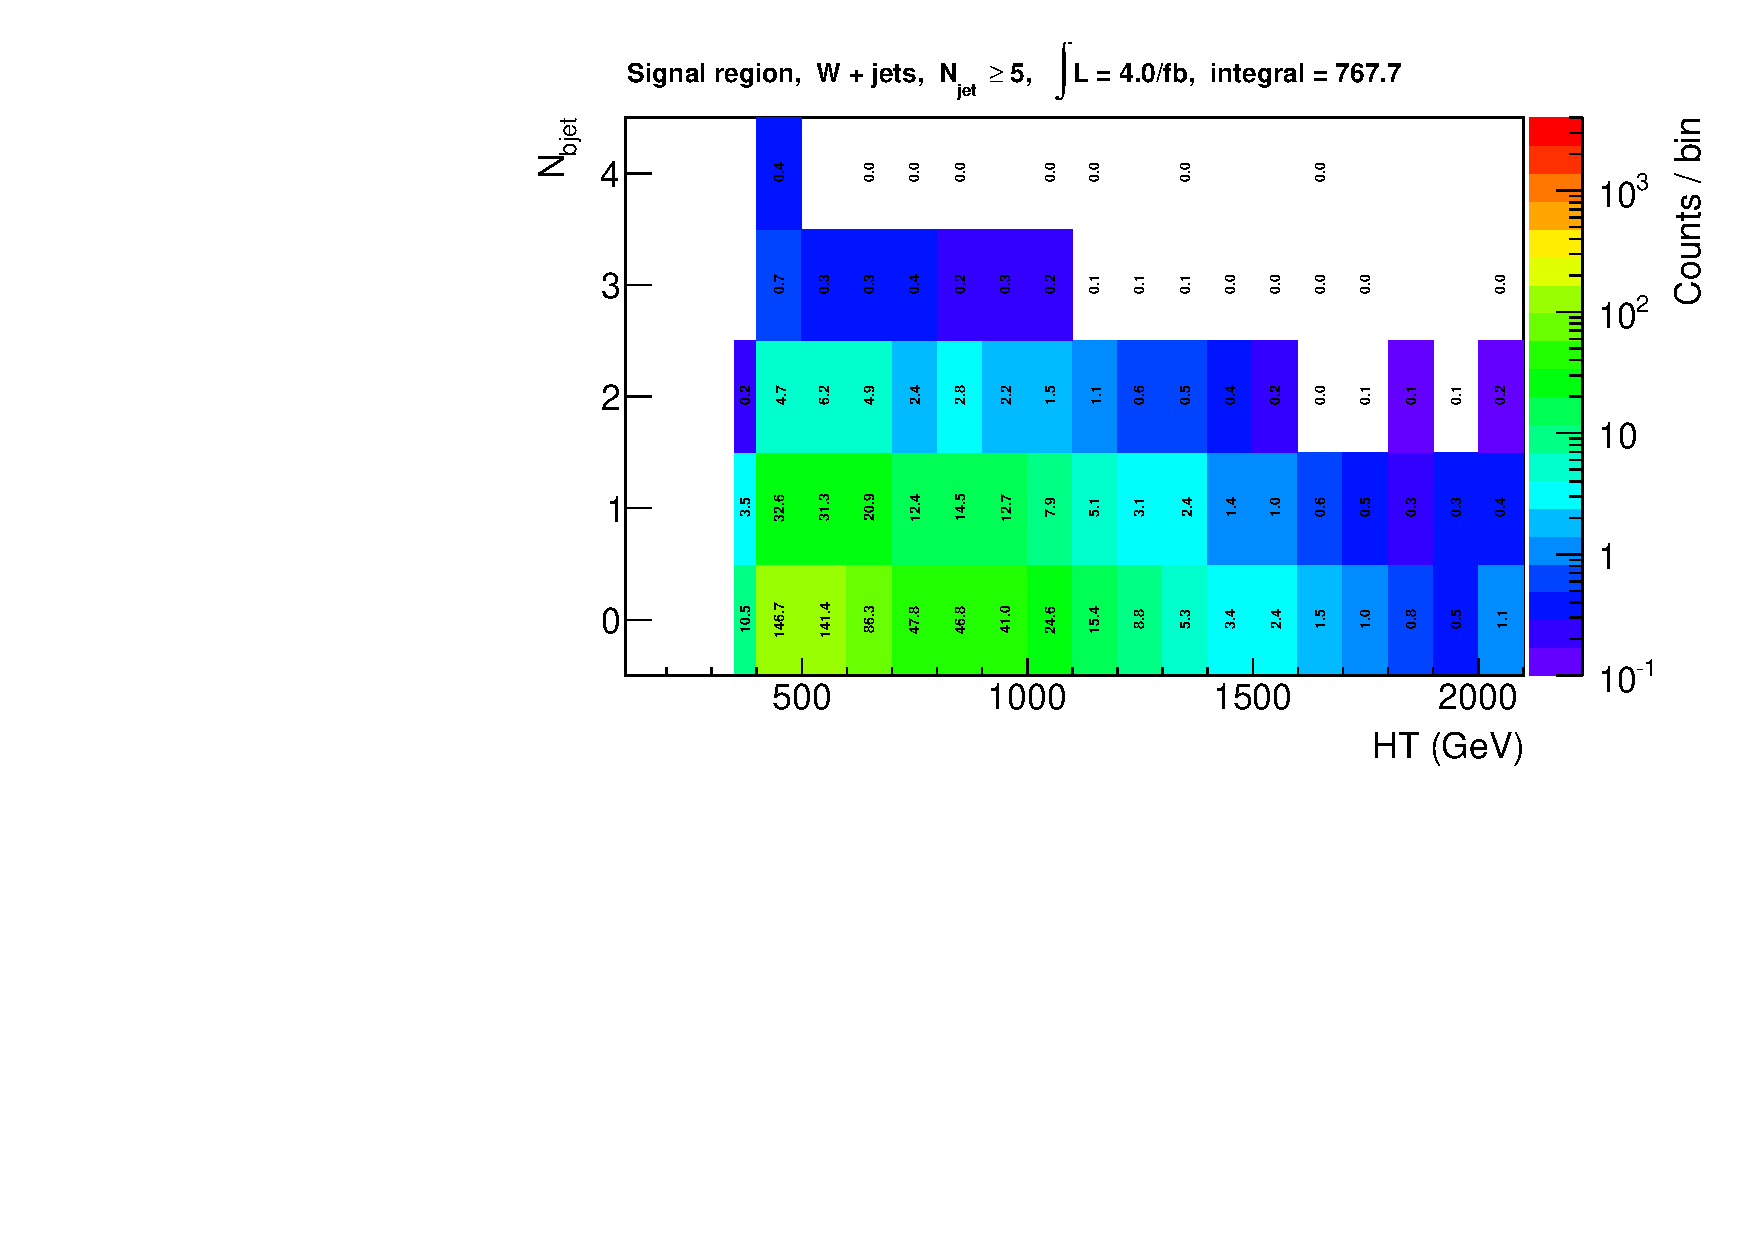
\includegraphics[width=0.5\textwidth]{figures/yieldPlots/had_wjets_ge5j.pdf}
  }~~
  \subfigure[Hadronic signal region yields for \ttbar background
  ($\njet \geq 5$)]{
    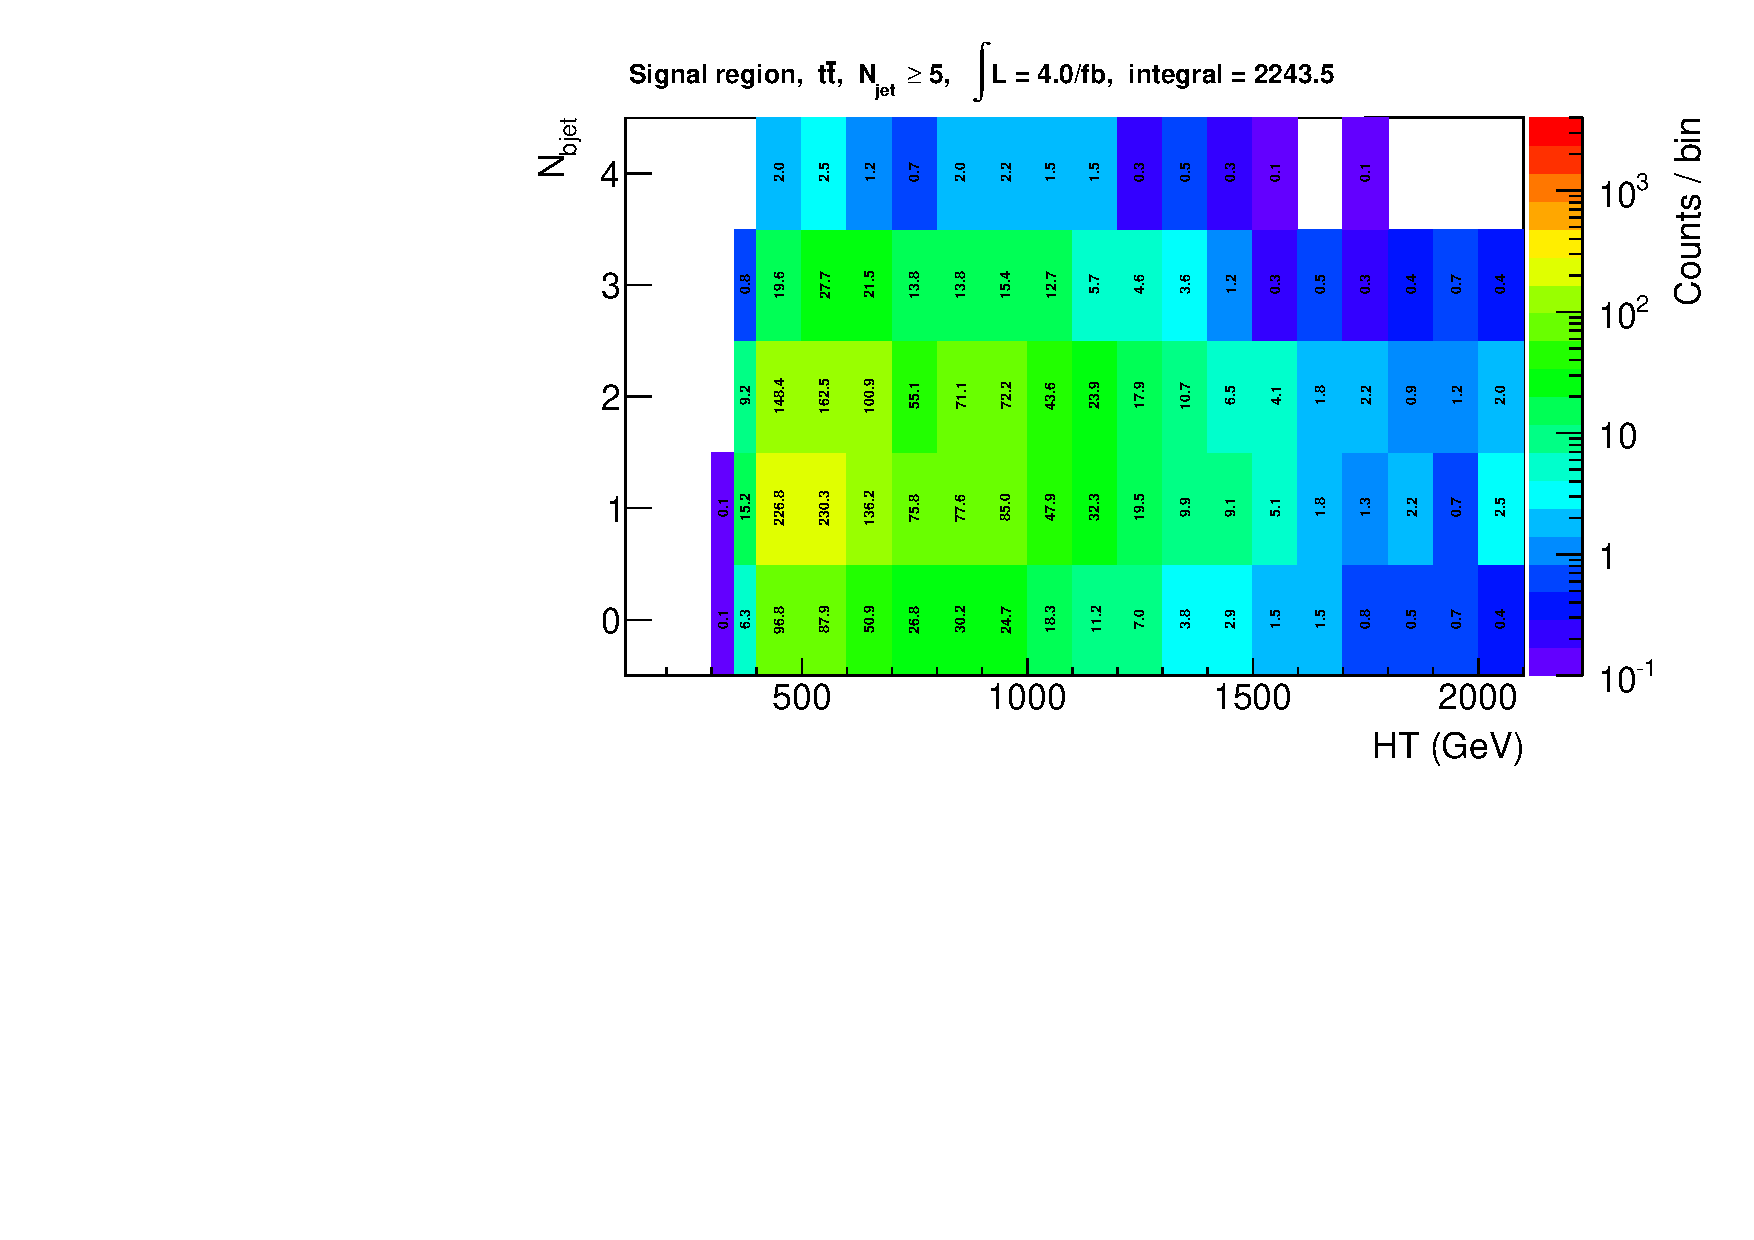
\includegraphics[width=0.5\textwidth]{figures/yieldPlots/had_ttbar_ge5j.pdf}
  }

  \\
  \subfigure[Hadronic signal region yields for T1bbbb simplified model 
  ($\njet \geq 5$)]{
    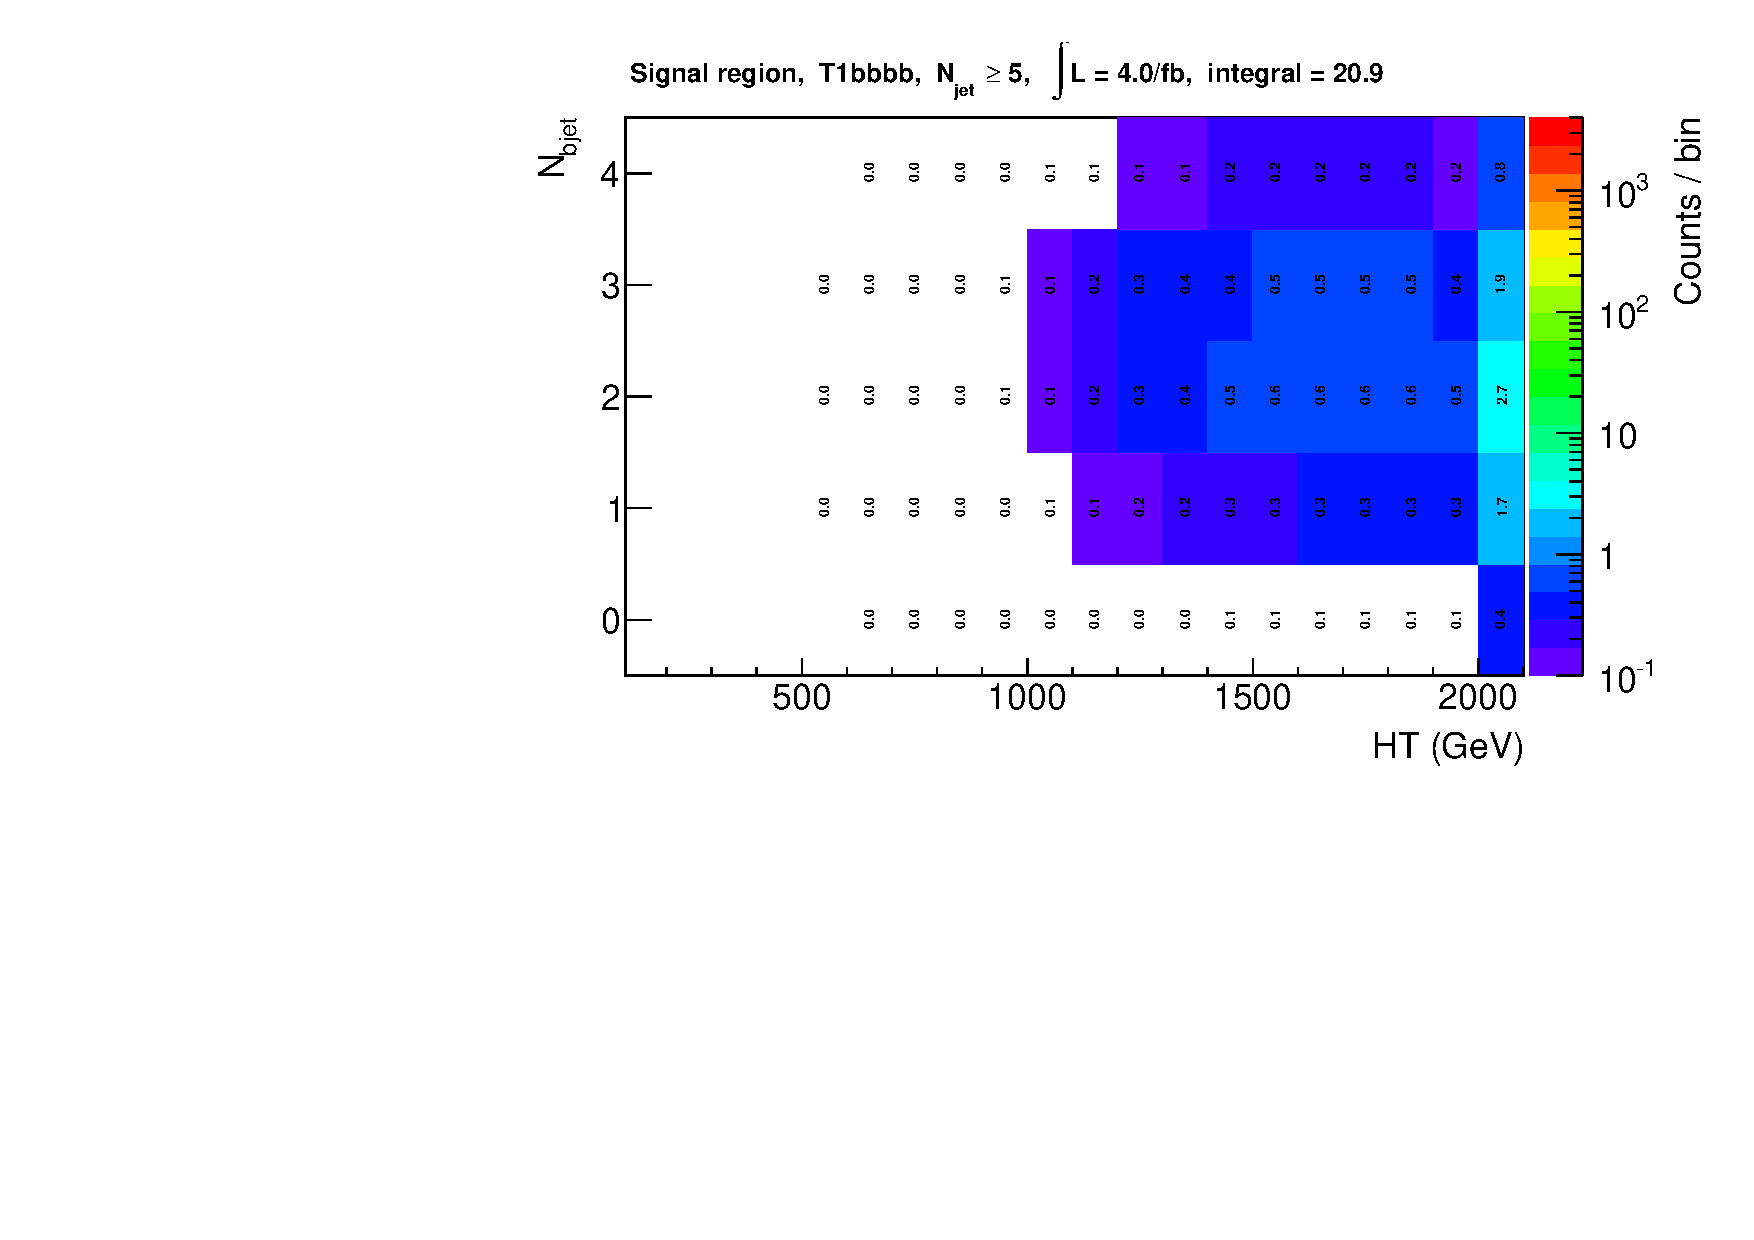
\includegraphics[width=0.5\textwidth]{figures/yieldPlots/sig_T1bbbb_ge5j.pdf}
  }
  \\
  \caption{\label{fig:ewkYields} Yields at $4\fbinv$ for the electroweak backgrounds in the
  hadronic signal region. Split up with the analysis bins. }
\end{figure}

%%____________________________________________________________________________||

\subsection{Definition of the control samples}
\label{sec:controlSelection}

\subsubsection{Hadronic control sample}

A disjoint hadronic control sample consisting predominantly of
multijet events is defined by applying the hadronic pre-selection
criteria and inverting the \alphat and/or \mhtmet requirements for a
given \scalht region, which is used primarily in the estimation of any
residual background from QCD multijet events, described in
Sec.~\ref{sec:qcd}.

\subsubsection{The \texorpdfstring{\mj}{muon plus jets} control sample}

Events from the \wj and \ttbar processes are found in the hadronic
signal sample due to unidentified leptons (either out of acceptance or
not reconstructed) and hadronic tau decays originating from
high-p$_{T}$ W bosons. An estimate of these background processes is
obtained through the use of a \mj sample. The selection criteria for
this sample are chosen to identify W bosons decaying to a muon and a
neutrino in the phase-space of the signal. The muon is not considered
in the calculation of event-level variables such as \scalht, \mht and
\alphat. All cuts on such jet-based quantities are consistent with
those applied in the hadronic search region and the same \njet, \nb,
and \scalht binning is used. The only exception is that no \alphat
requirement is made, as motivated by the discussion in
Sec.~\ref{sec:larger}. In order to select events containing W bosons,
exactly one tight isolated muon within an acceptance of \PT $>$ 30
\gev and $|\eta| <$ 2.1 is required (due to the trigger), and the
transverse mass of the W candidate must satisfy $30 < \mt(\mu,\pfmet)
< 125\gev$ (to suppress QCD multijet and potential signal
events). Events are vetoed if $\Delta R(\mu,\textrm{jet}_i) < 0.5$
running over all jets $i$. The single isolated track veto, described
in Sections~\ref{sec:reconstruction} and~\ref{sec:vetoes}, is also
applied, which considers all single isolated tracks in the event
except that associated with the identified, isolated muon. Finally,
the cleaning cut $\mht/\pfmet$ is also applied, as done in the signal
region, where the \pfmet is adjusted to account for the transverse
momentum of the identified, isolated muon.

%STACK THESE UP
\begin{figure}[h!]
  \centering
  \subfigure[Yields from \texorpdfstring{\mj}{muon plus jets} control sample
  ($\njet = 2$)]{
    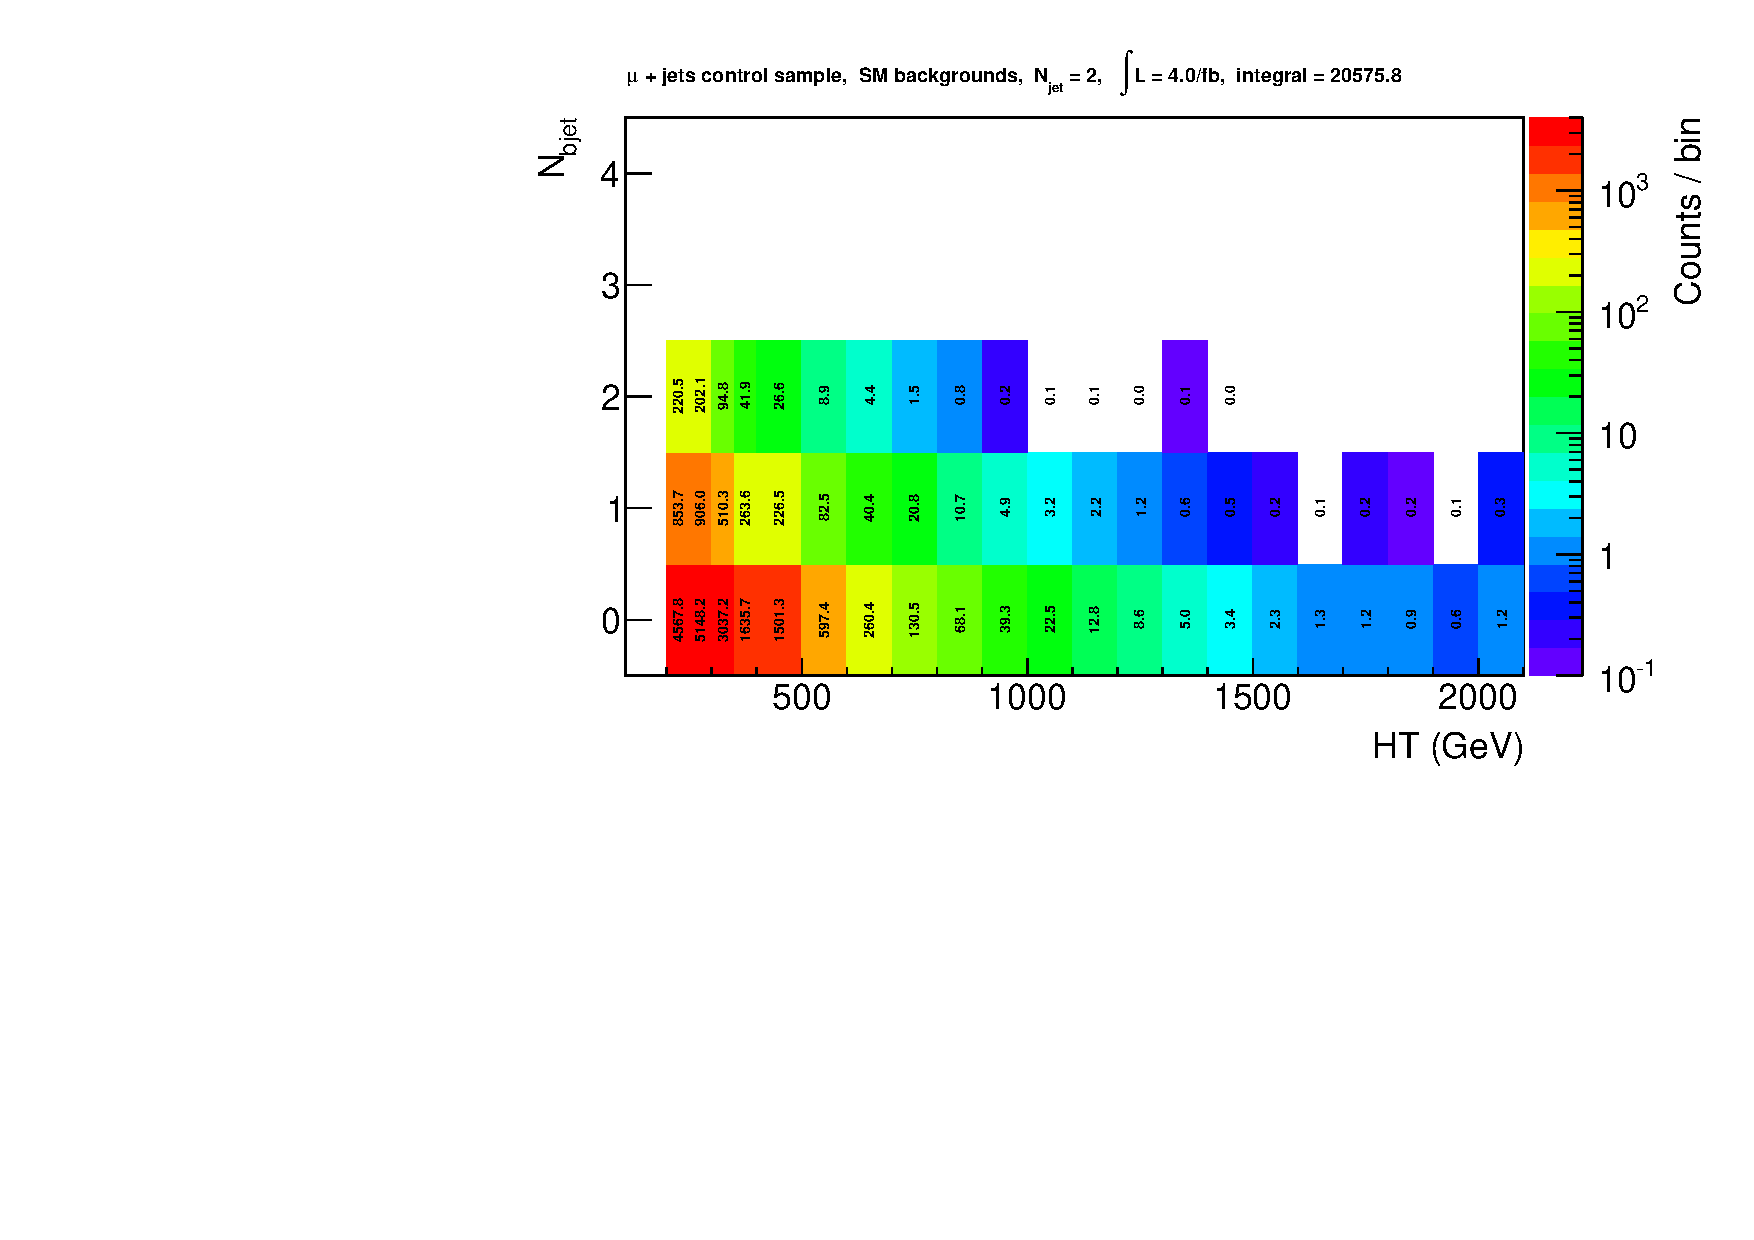
\includegraphics[width=0.5\textwidth]{figures/yieldPlots/mu_ewk_eq2j.pdf}
  }~~
  \subfigure[Yields from \texorpdfstring{\mj}{muon plus jets} control sample
  ($\njet = 3$)]{
    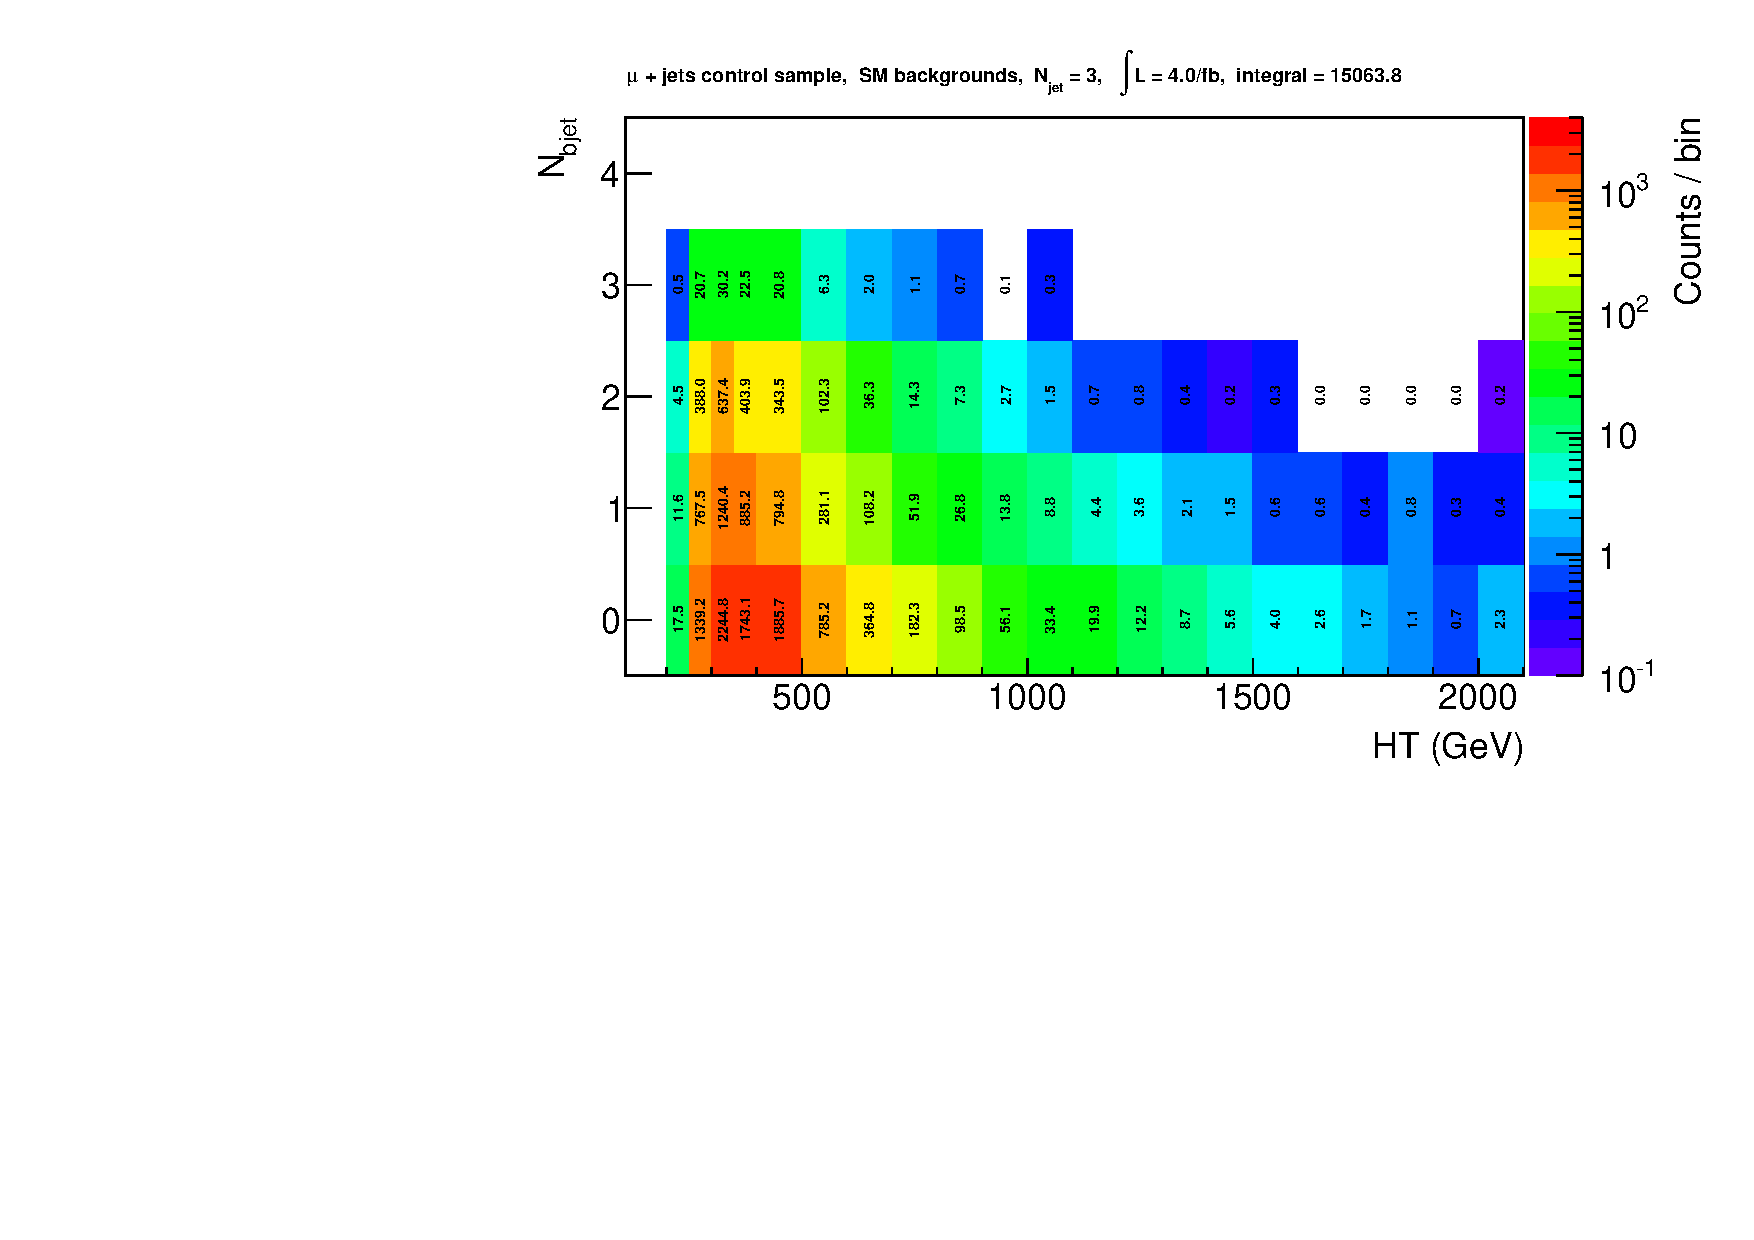
\includegraphics[width=0.5\textwidth]{figures/yieldPlots/mu_ewk_eq3j.pdf}
  }
  \\
  \subfigure[Yields from \texorpdfstring{\mj}{muon plus jets} control sample
  ($\njet = 4$)]{
    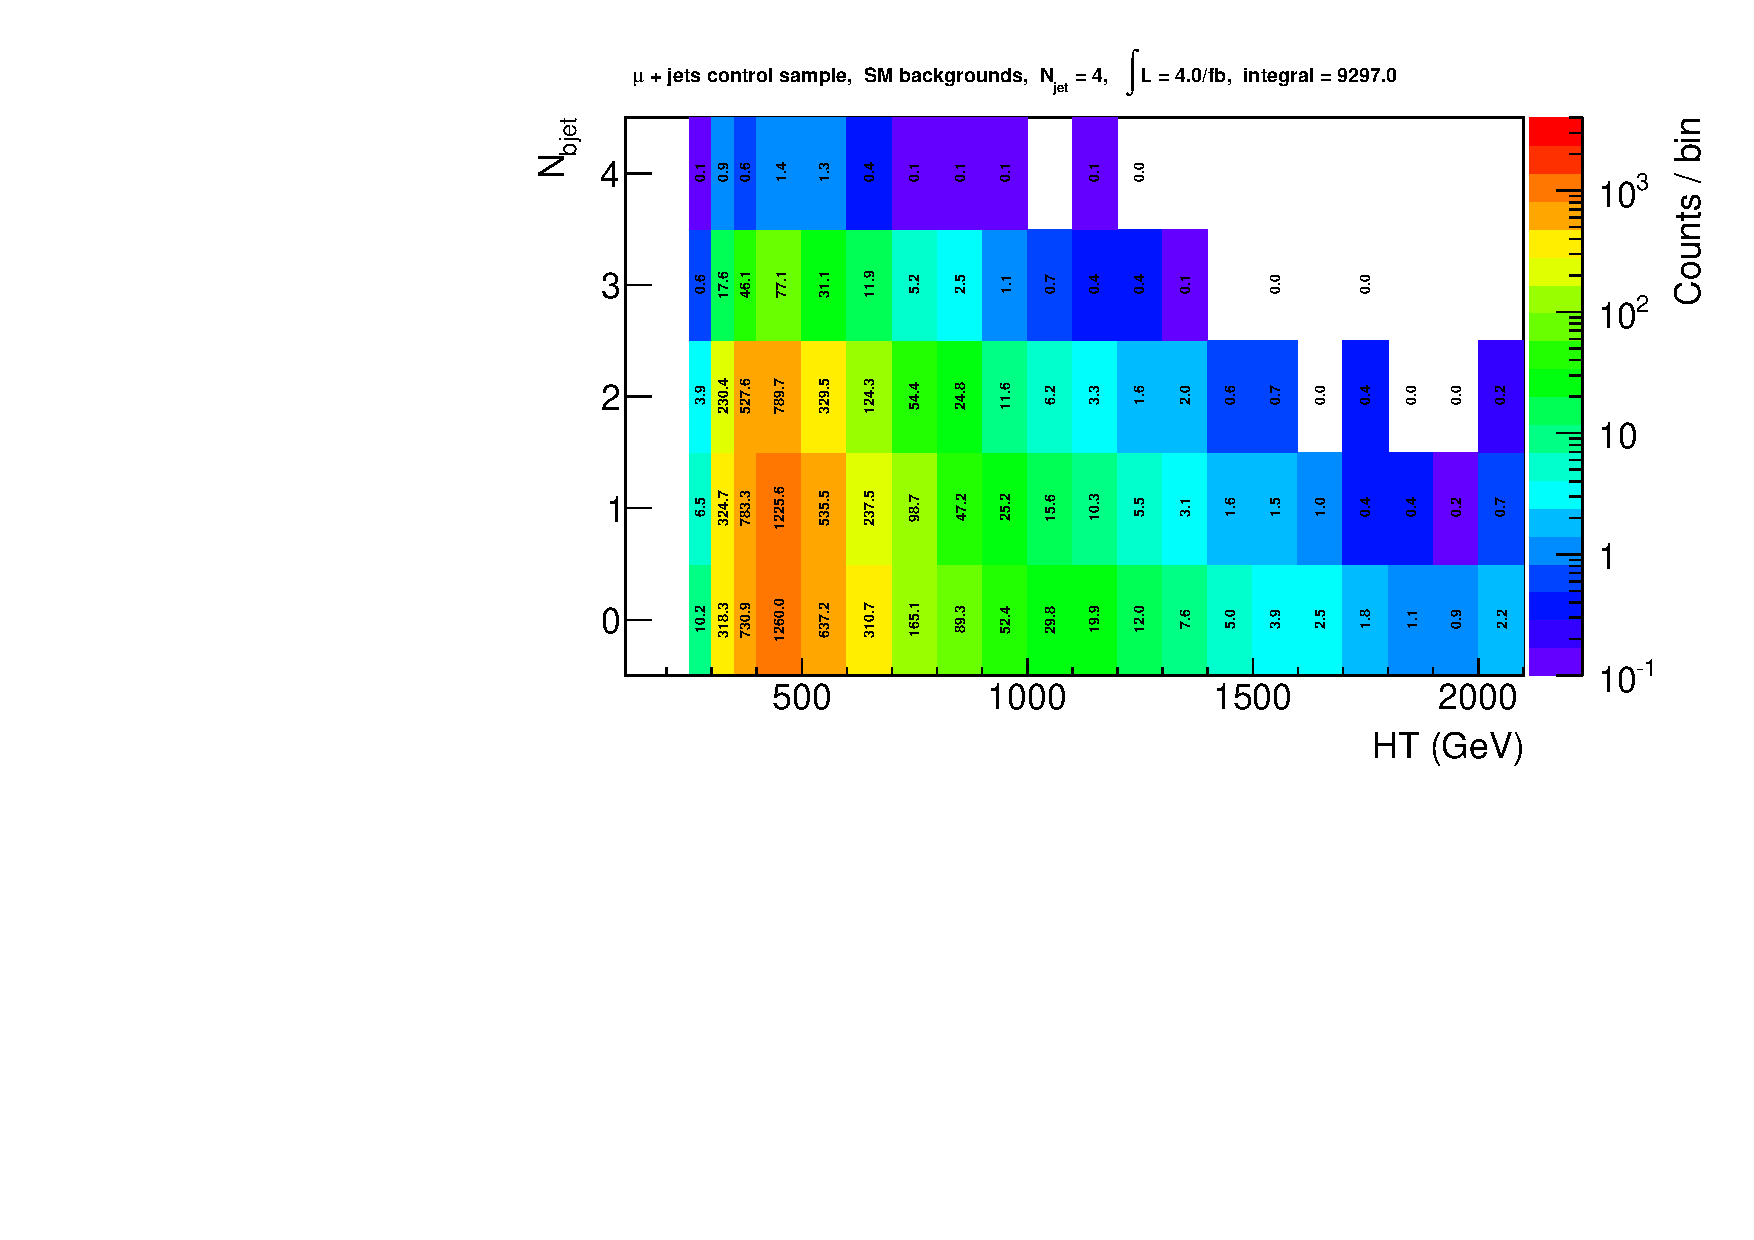
\includegraphics[width=0.5\textwidth]{figures/yieldPlots/mu_ewk_eq4j.pdf}
  }~~
  \subfigure[Yields from \texorpdfstring{\mj}{muon plus jets} control sample
  ($\njet \geq 5$)]{
    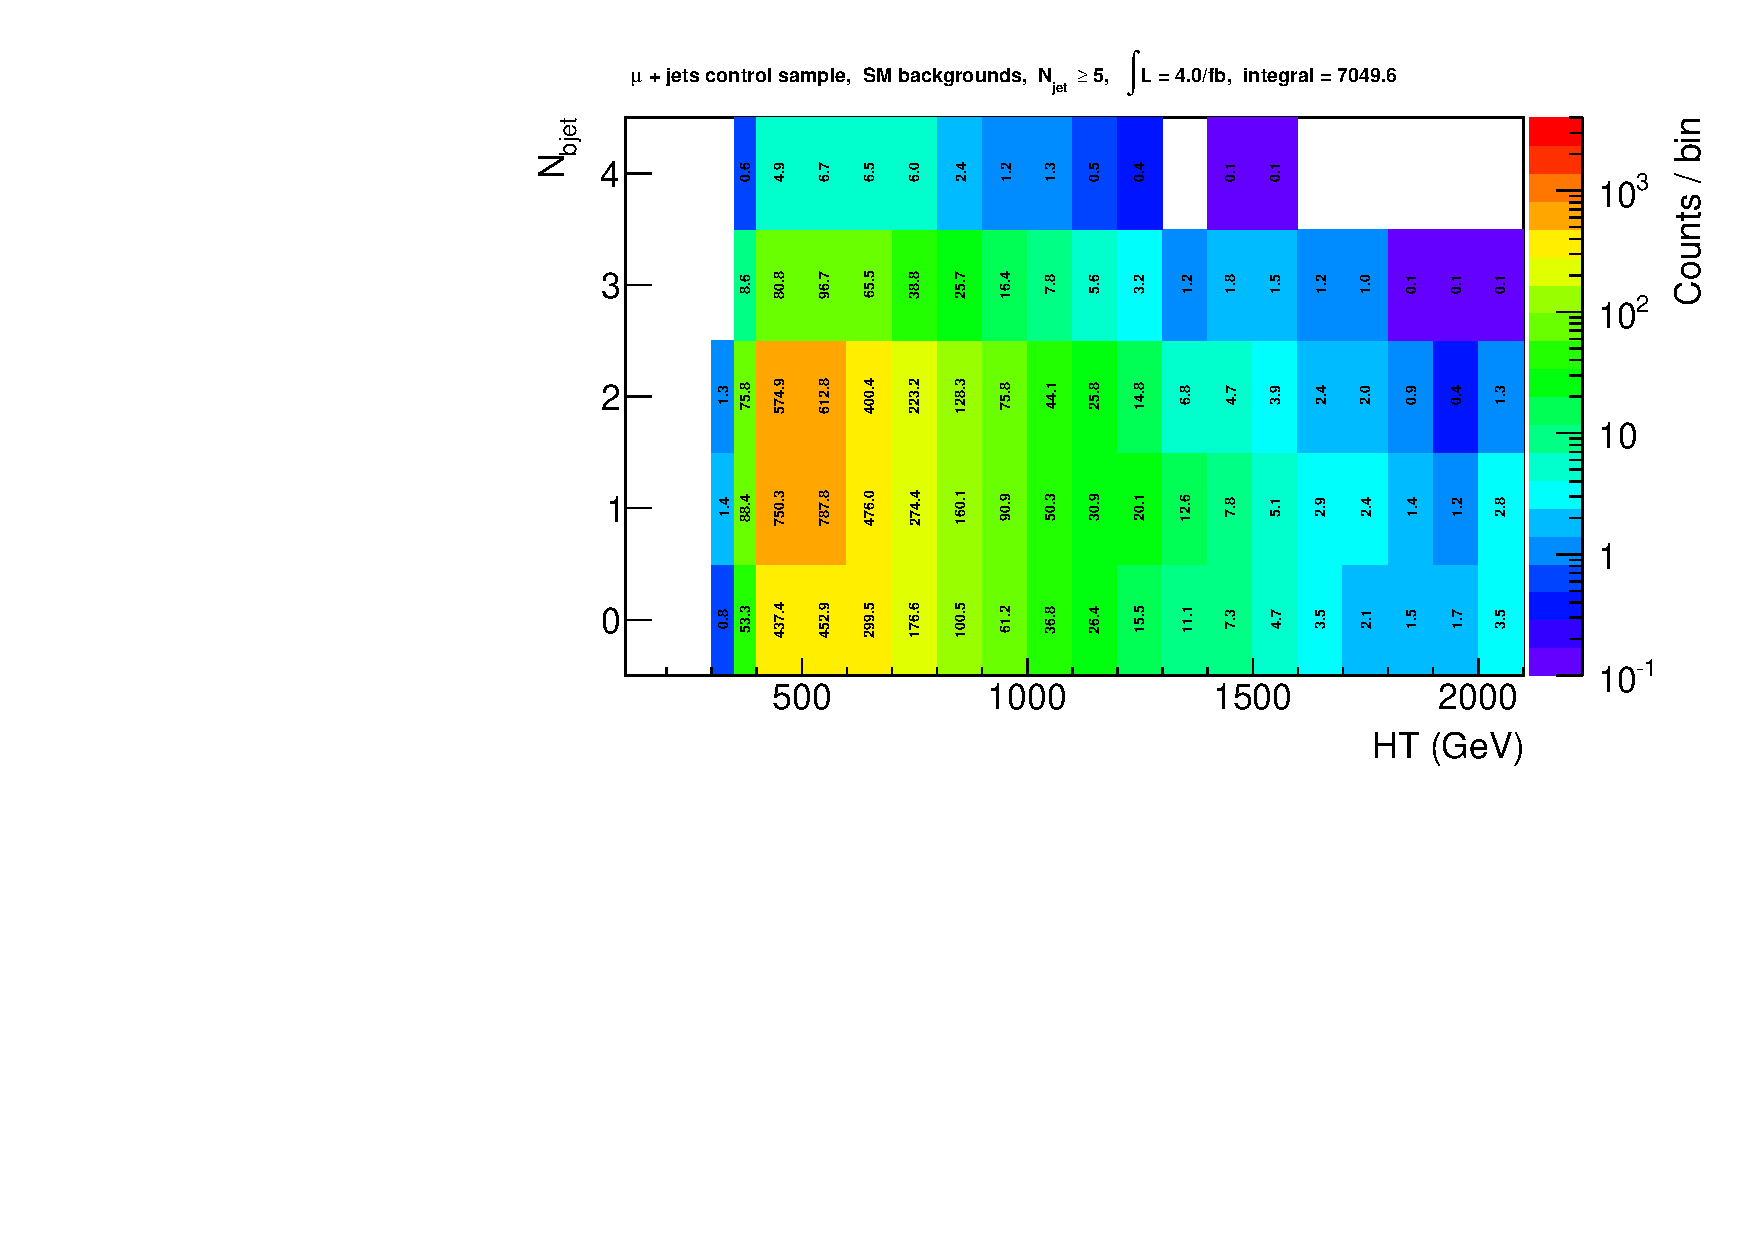
\includegraphics[width=0.5\textwidth]{figures/yieldPlots/mu_ewk_ge5j.pdf}
  } 
  \\
  \caption{\label{fig:ewkYields} Yields at $4\fbinv$ for the W~+~jets and \ttbar
  MC contributions to the \texorpdfstring{\mj}{muon plus jets} control sample. }
\end{figure}


\subsubsection{The \texorpdfstring{\mmj}{di-muon plus jets} control sample}

The \znunu\ + jets process forms an irreducible background and can be
estimated using the \zmumu + jets process, which has similar kinematic
properties but a different acceptance and a smaller branching ratio. A
background estimate is obtained through the use of a \mmj sample. Most
of the selection criteria are identical to those for the \mj sample,
but the few that differ are tuned to identify Z bosons decaying to two
muons in the kinematic phase space of the signal region. The muons are
not considered in the calculation of event-level variables such as
\scalht, \mht and \alphat. All cuts on such jet-based quantities are
consistent with those applied in the hadronic search region and the
same \njet, \nb, and \scalht binning is used. The only exception is
that no \alphat requirement is made, as motivated by the discussion in
Sec.~\ref{sec:larger}. In order to select an event sample containing Z
bosons, exactly two tight isolated muons within an acceptance of $\Pt
> 30\gev$ and $|\eta| < 2.1$ are required (due to the trigger). The
invariant mass of the two muons must satisfy $m_{Z} - 25 <
M_{\mu_1\mu_2} < m_{Z} + 25$. Events are vetoed if $\Delta
R(\mu_{i},\textrm{jet}_j) < 0.5$ is satisfied, running over all muons
$i$ and all jets $j$. The single isolated track veto, described in
Sections~\ref{sec:reconstruction} and~\ref{sec:vetoes}, is also
applied, considering all single isolated tracks in the event except
those associated with the two identified, isolated muons. Finally, the
cleaning cut $\mht/\pfmet$ is also applied, as done in the signal
region, where the \pfmet is adjusted to account for the transverse
momenta of the two identified, isolated muons. The \mmj sample can be
used to make predictions in all the \scalht bins, providing coverage
at low \scalht where the \gj sample cannot.

\begin{figure}[h!]
  \centering
  \subfigure[Yields from \texorpdfstring{\mmj}{di-muon plus jets} control sample
  ($\njet = 2$)]{
    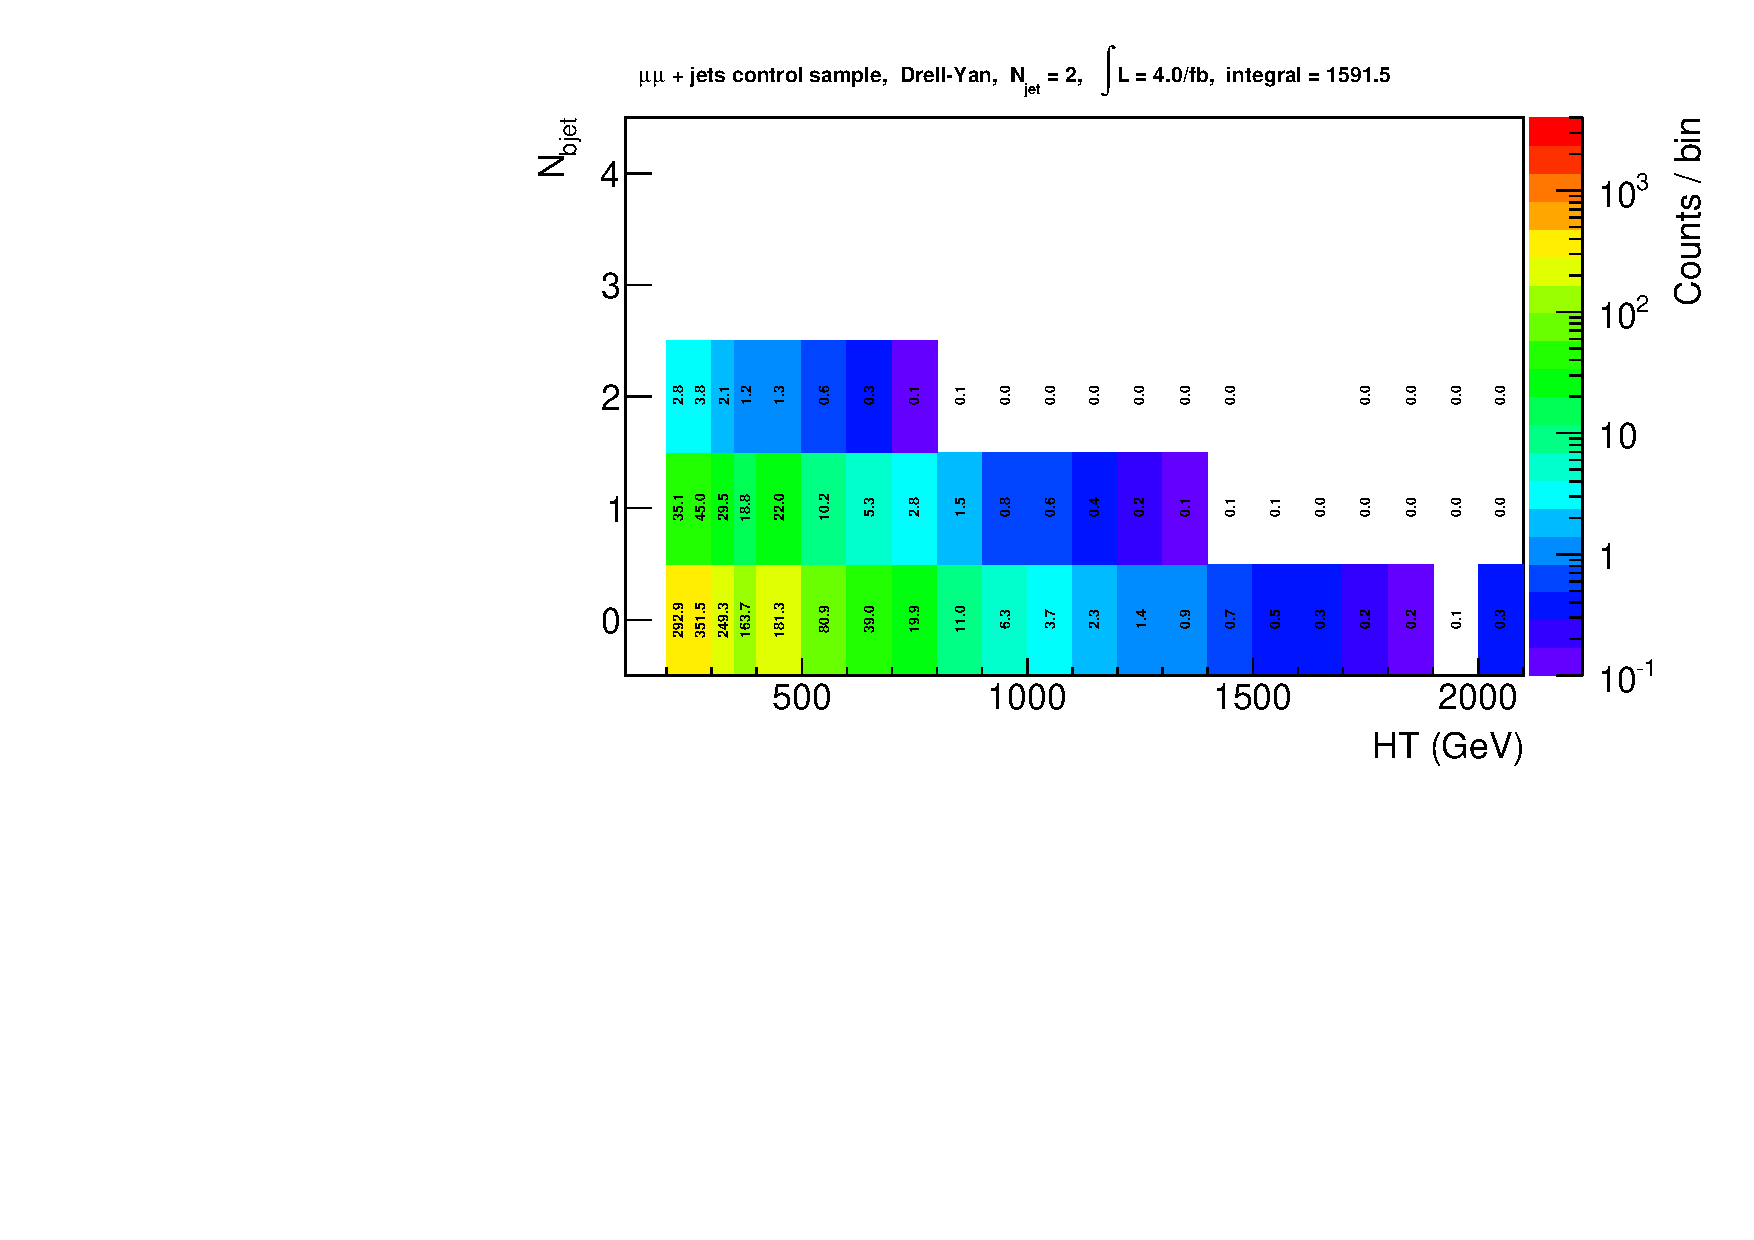
\includegraphics[width=0.5\textwidth]{figures/yieldPlots/mm_dy_eq2j.pdf}
  }~~
  \subfigure[Yields from \texorpdfstring{\mmj}{di-muon plus jets} control sample
  ($\njet = 3$)]{
    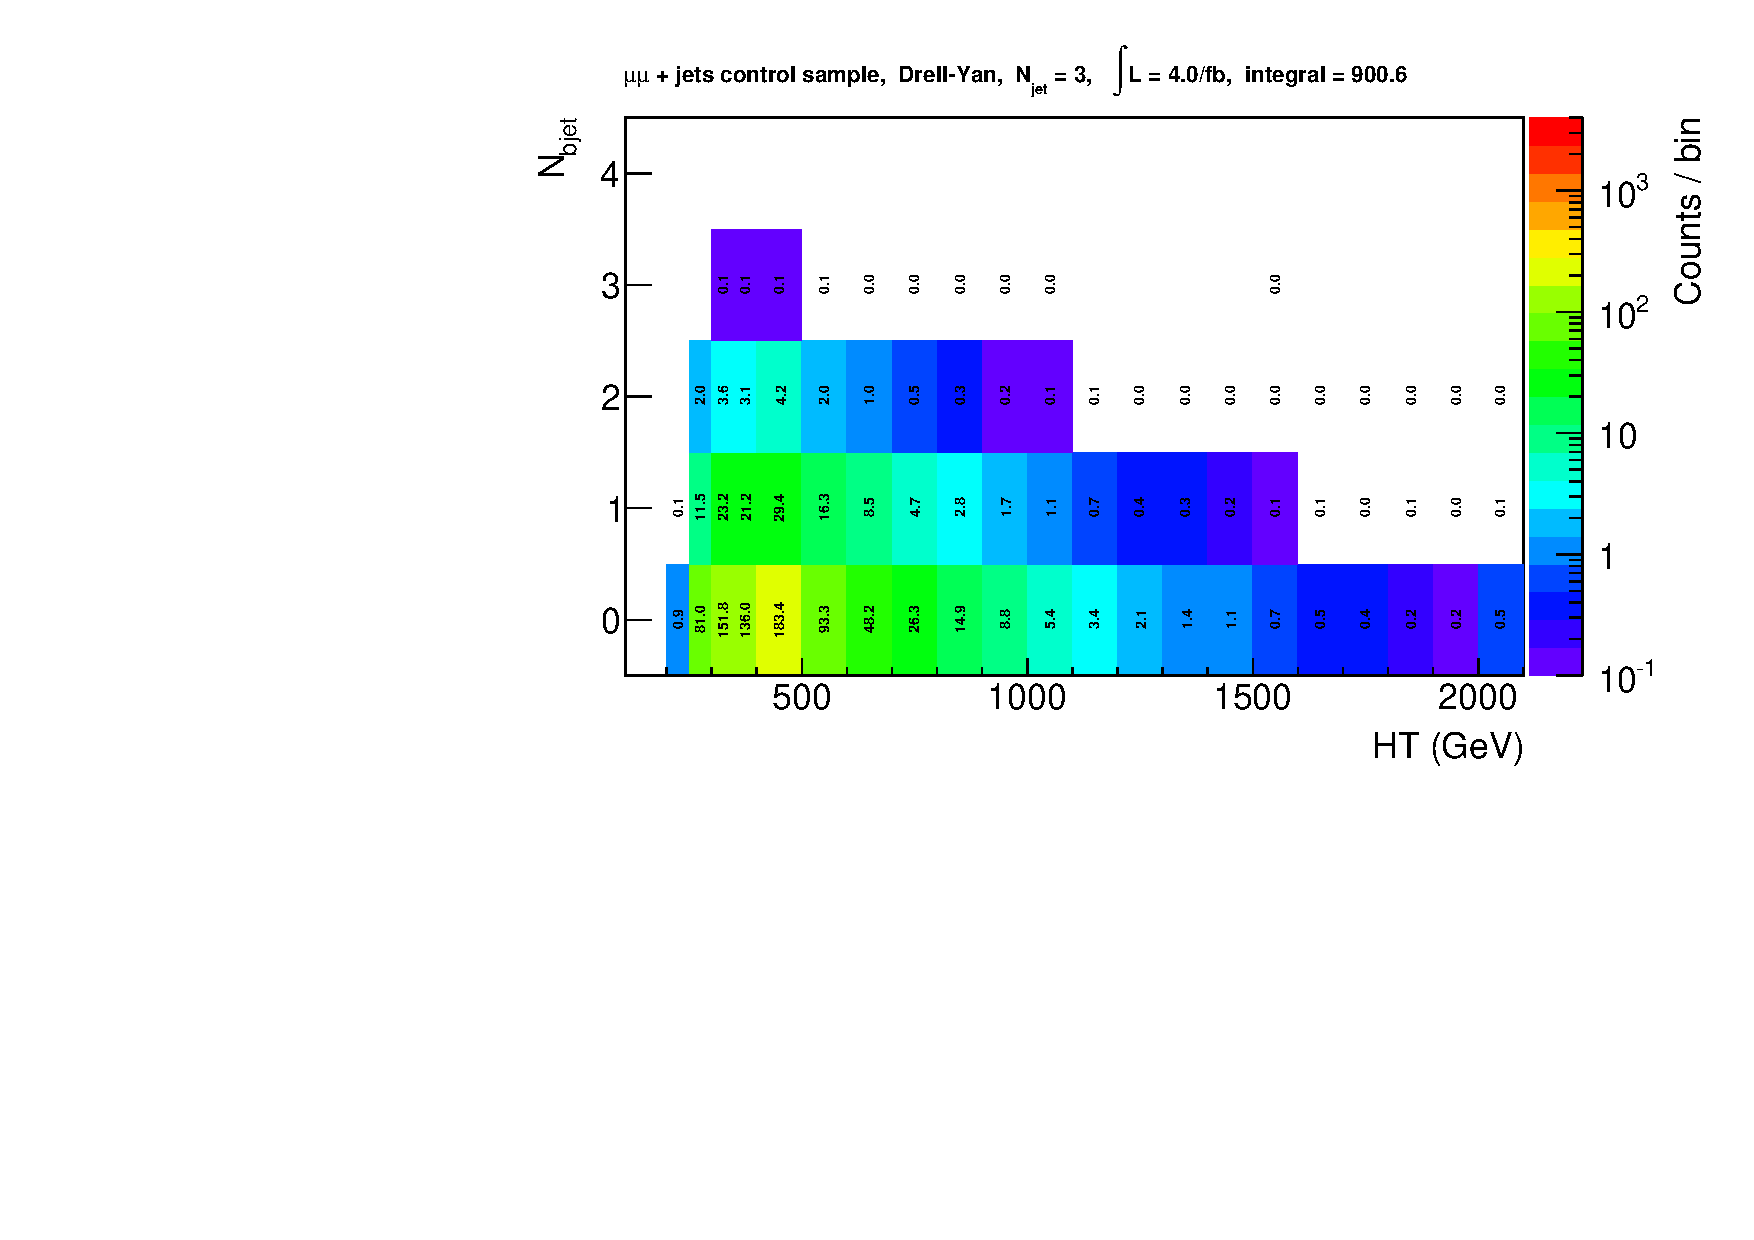
\includegraphics[width=0.5\textwidth]{figures/yieldPlots/mm_dy_eq3j.pdf}
  }
  \\
  \subfigure[Yields from \texorpdfstring{\mmj}{di-muon plus jets} control sample
  ($\njet = 4$)]{
    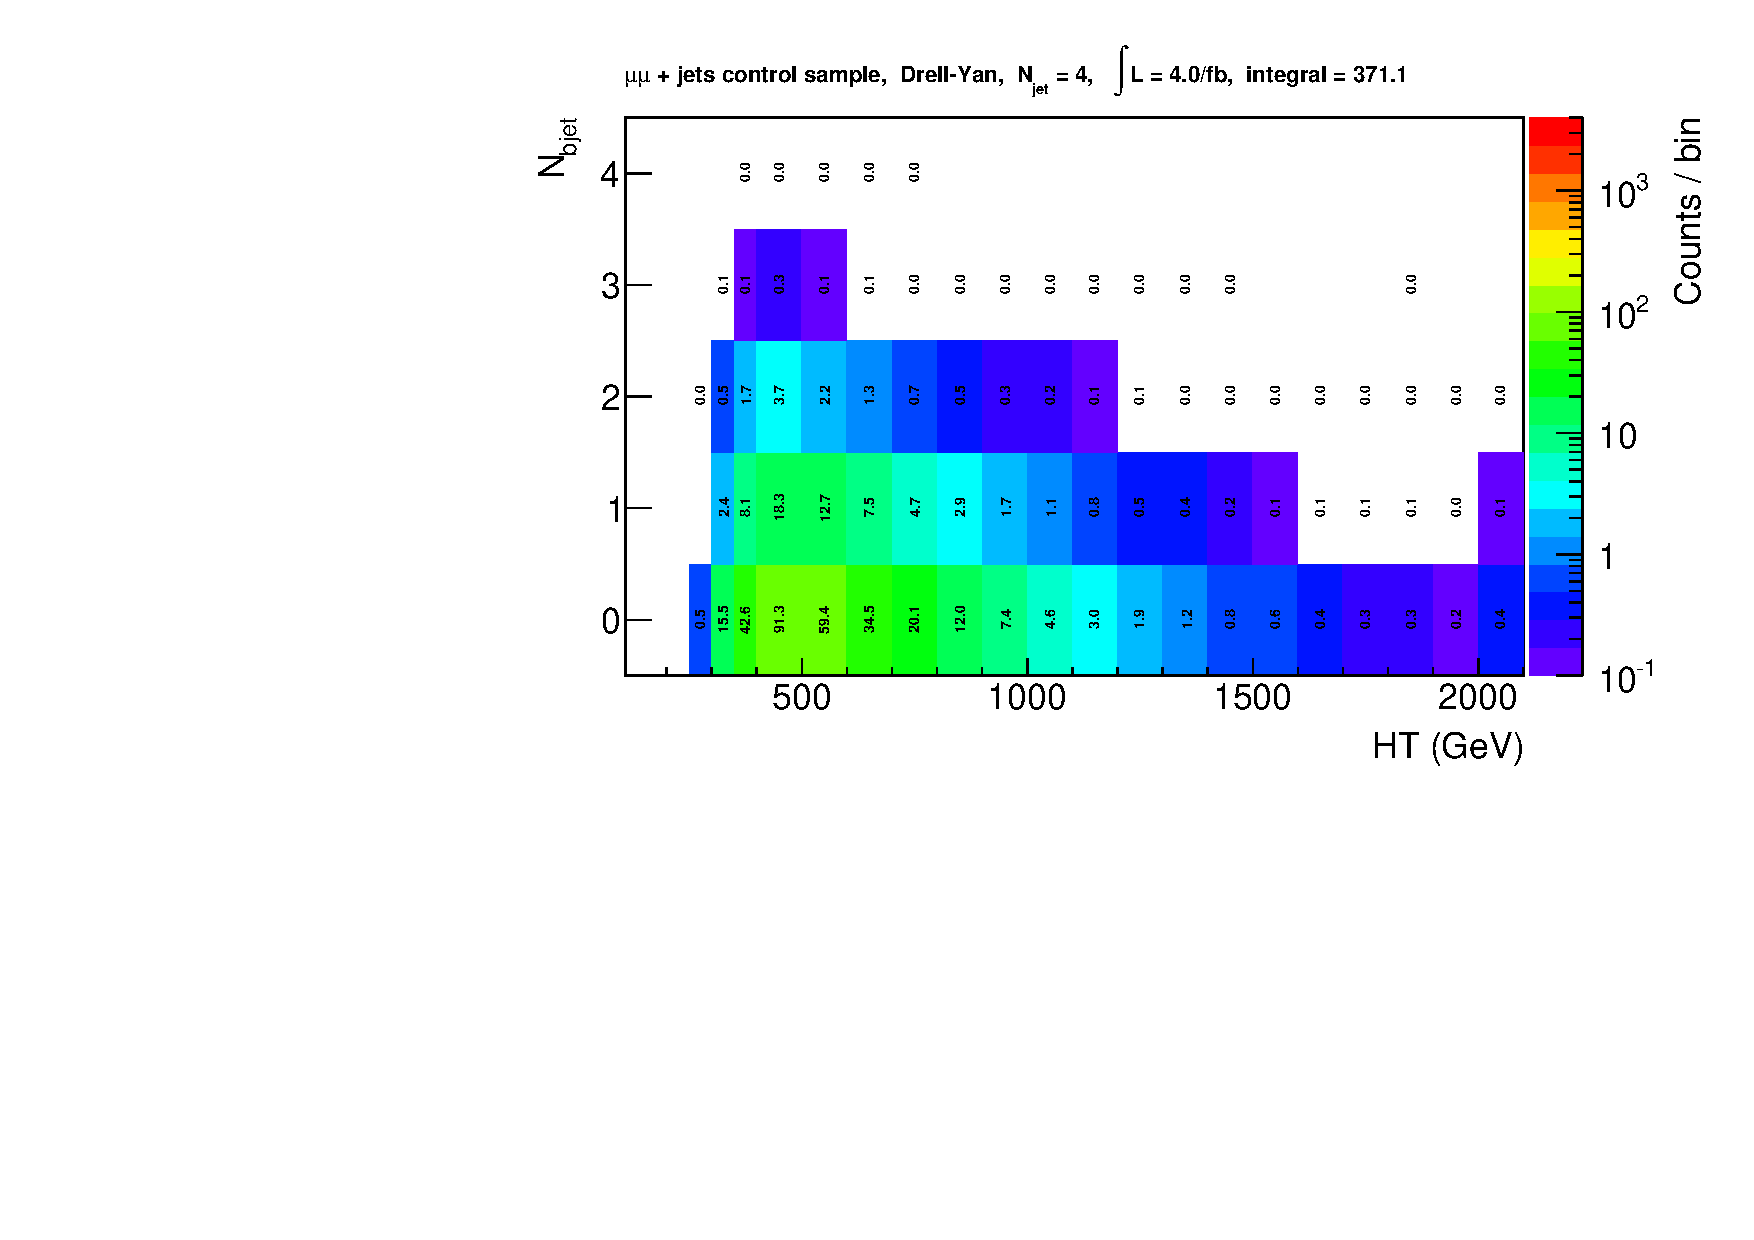
\includegraphics[width=0.5\textwidth]{figures/yieldPlots/mm_dy_eq4j.pdf}
  }~~
  \subfigure[Yields from \texorpdfstring{\mmj}{di-muon plus jets} control sample
  ($\njet \geq 5$)]{
    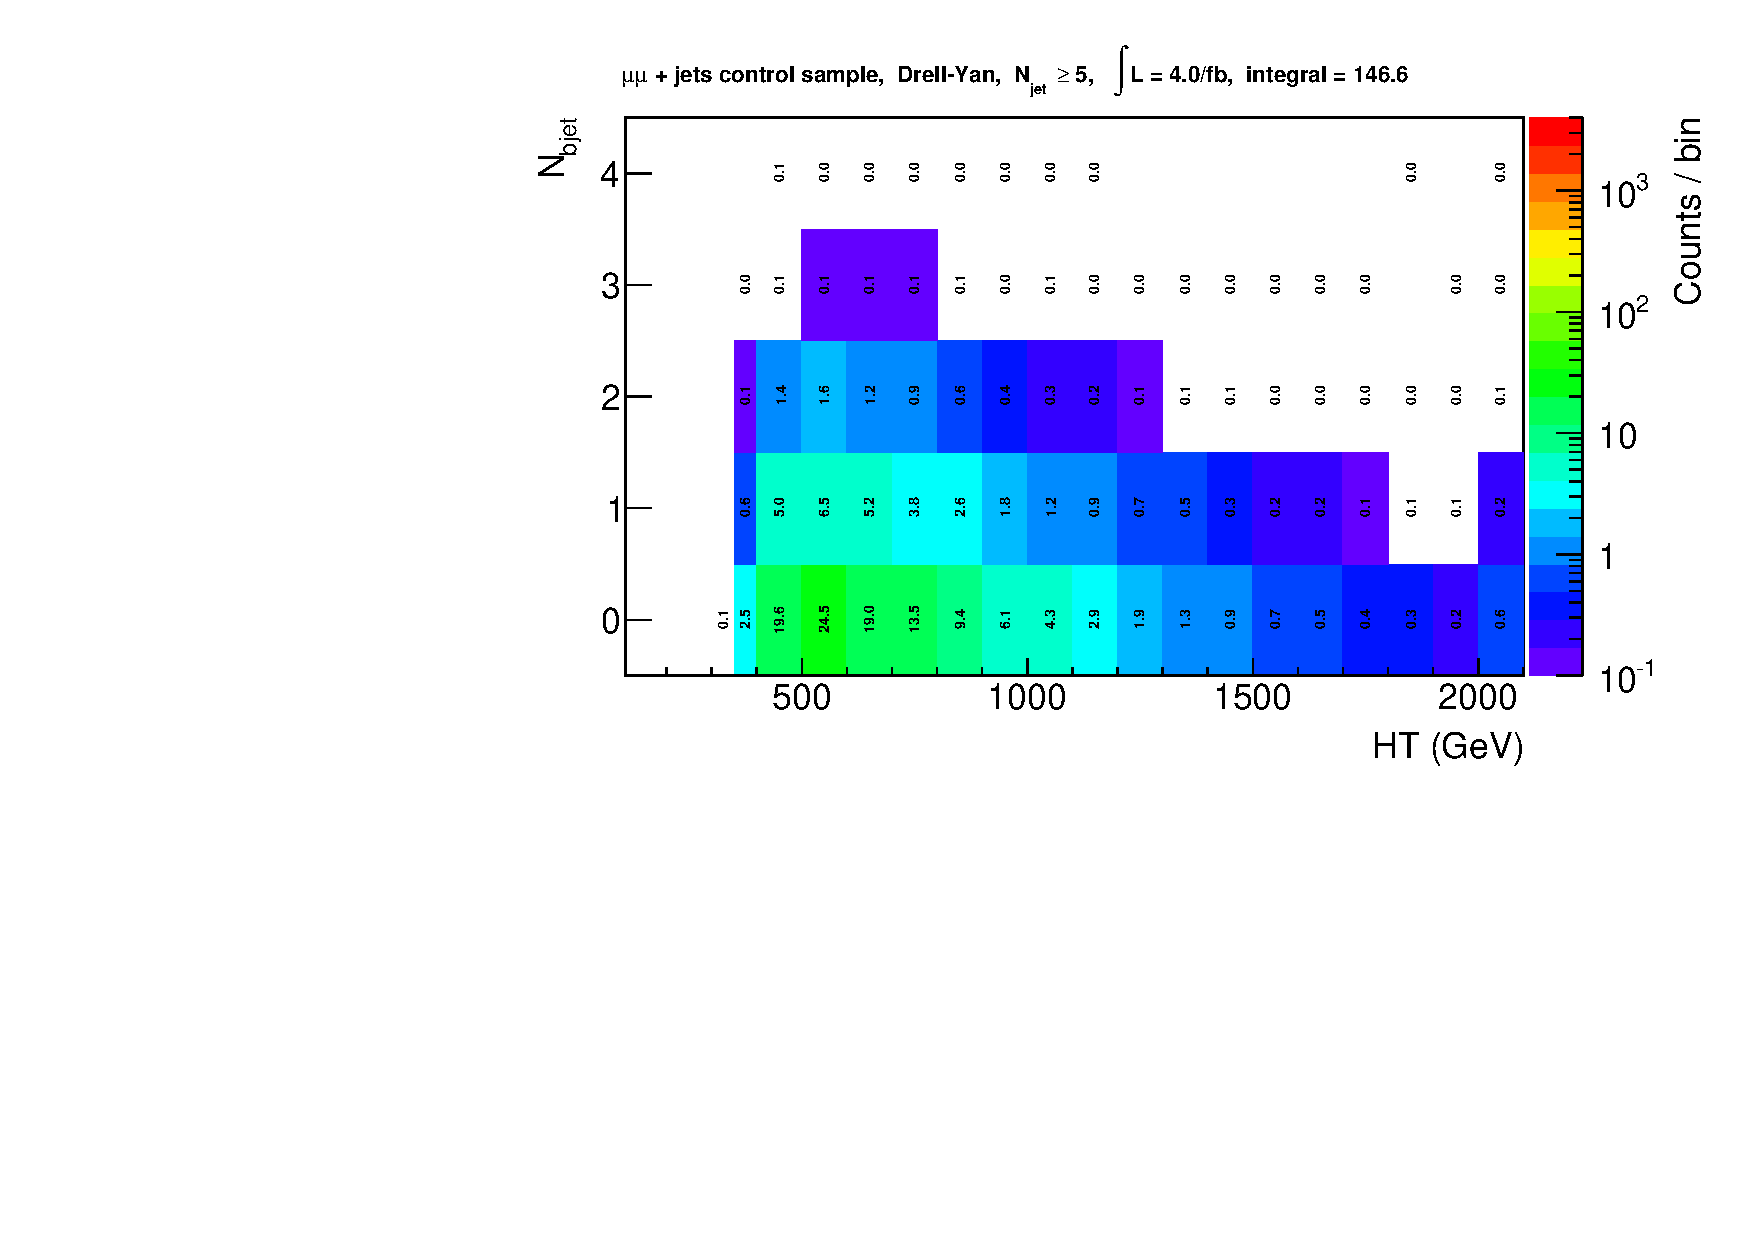
\includegraphics[width=0.5\textwidth]{figures/yieldPlots/mm_dy_ge5j.pdf}
  } 
  \\
  \caption{\label{fig:ewkYields} Yields at $4\fbinv$ for the DY~+~jets MC 
  contributions to the \texorpdfstring{\mmj}{di-muon plus jets} control sample. }
\end{figure}

\subsubsection{The \texorpdfstring{\gj}{photon plus jets} control sample}

The \znunu\ + jets process can also be estimated using the \gj
process, which has a larger cross section and kinematic properties
similar to those of \znunu\ events when the photon is
ignored~\cite{PAS-SUS-08-002,Bern:2011pa}. The \gj sample is defined
by requiring exactly one photon satisfying tight isolation criteria
and within an acceptance of $\pt > 175\gev$ and $|\eta| <
1.45$ (the anticipated limitation from the trigger). Furthermore, events are vetoed if $\Delta
R(\gamma,\textrm{jet}_j) < 1.0$ is satisfied, running over all jets
$j$. As for the muon-based samples, the photon is not considered in
the calculation of event-level variables such as \scalht, \mht, \met and 
\alphat. All cuts on jet-based quantities are consistent with those
applied in the hadronic search region, and the same \HT binning is
used. 
% Given that the photon is ignored, the \gj sample can only be
% used for the region $\scalht > 375\gev$ due to the photon acceptance
% of $\pt > 165\gev$ (enforced by the trigger) and the requirement
% $\alphat > 0.55$.

\begin{figure}[h!]
  \centering
  \subfigure[Yields from \texorpdfstring{\gj}{photon plus jets} control sample
  ($\njet = 2$)]{
    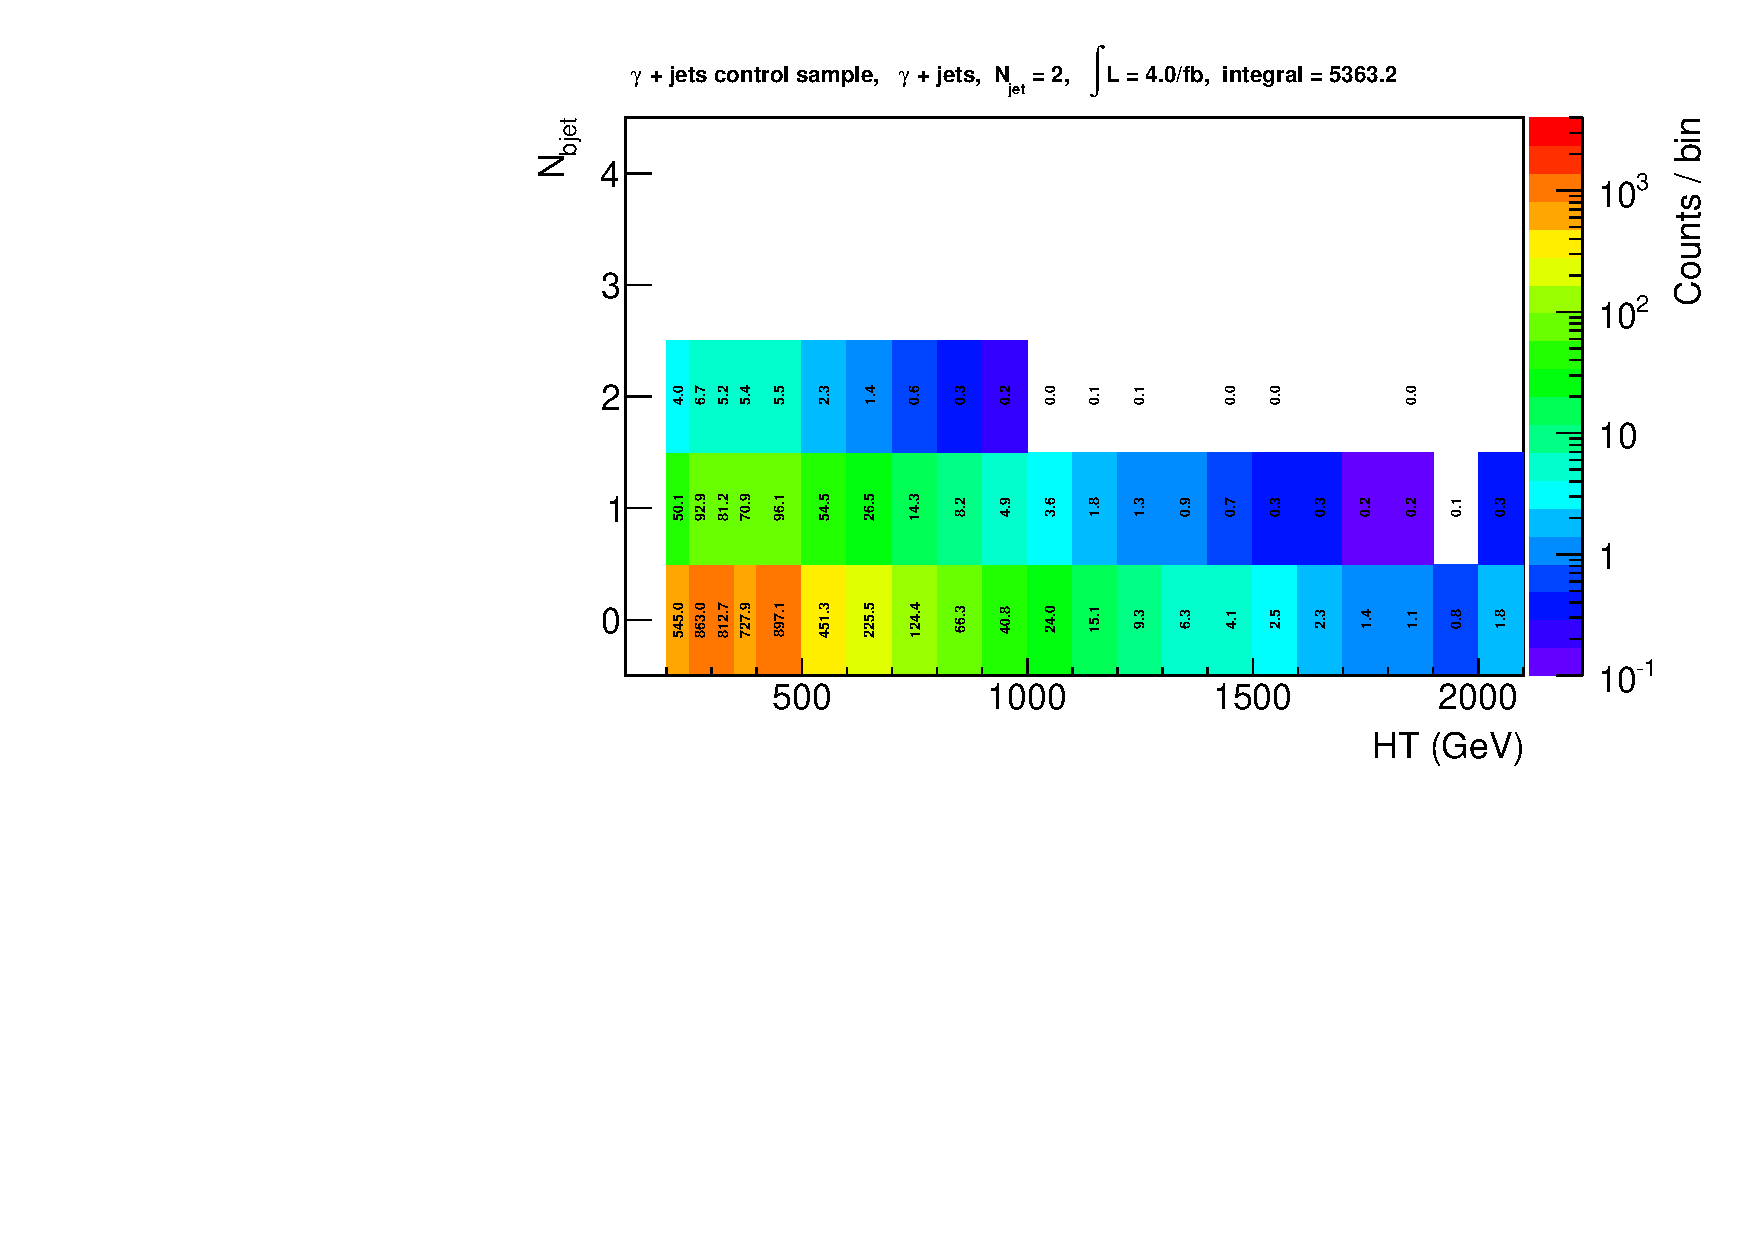
\includegraphics[width=0.5\textwidth]{figures/yieldPlots/ph_gjets_eq2j.pdf}
  }~~
  \subfigure[Yields from \texorpdfstring{\gj}{photon plus jets} control sample
  ($\njet = 3$)]{
    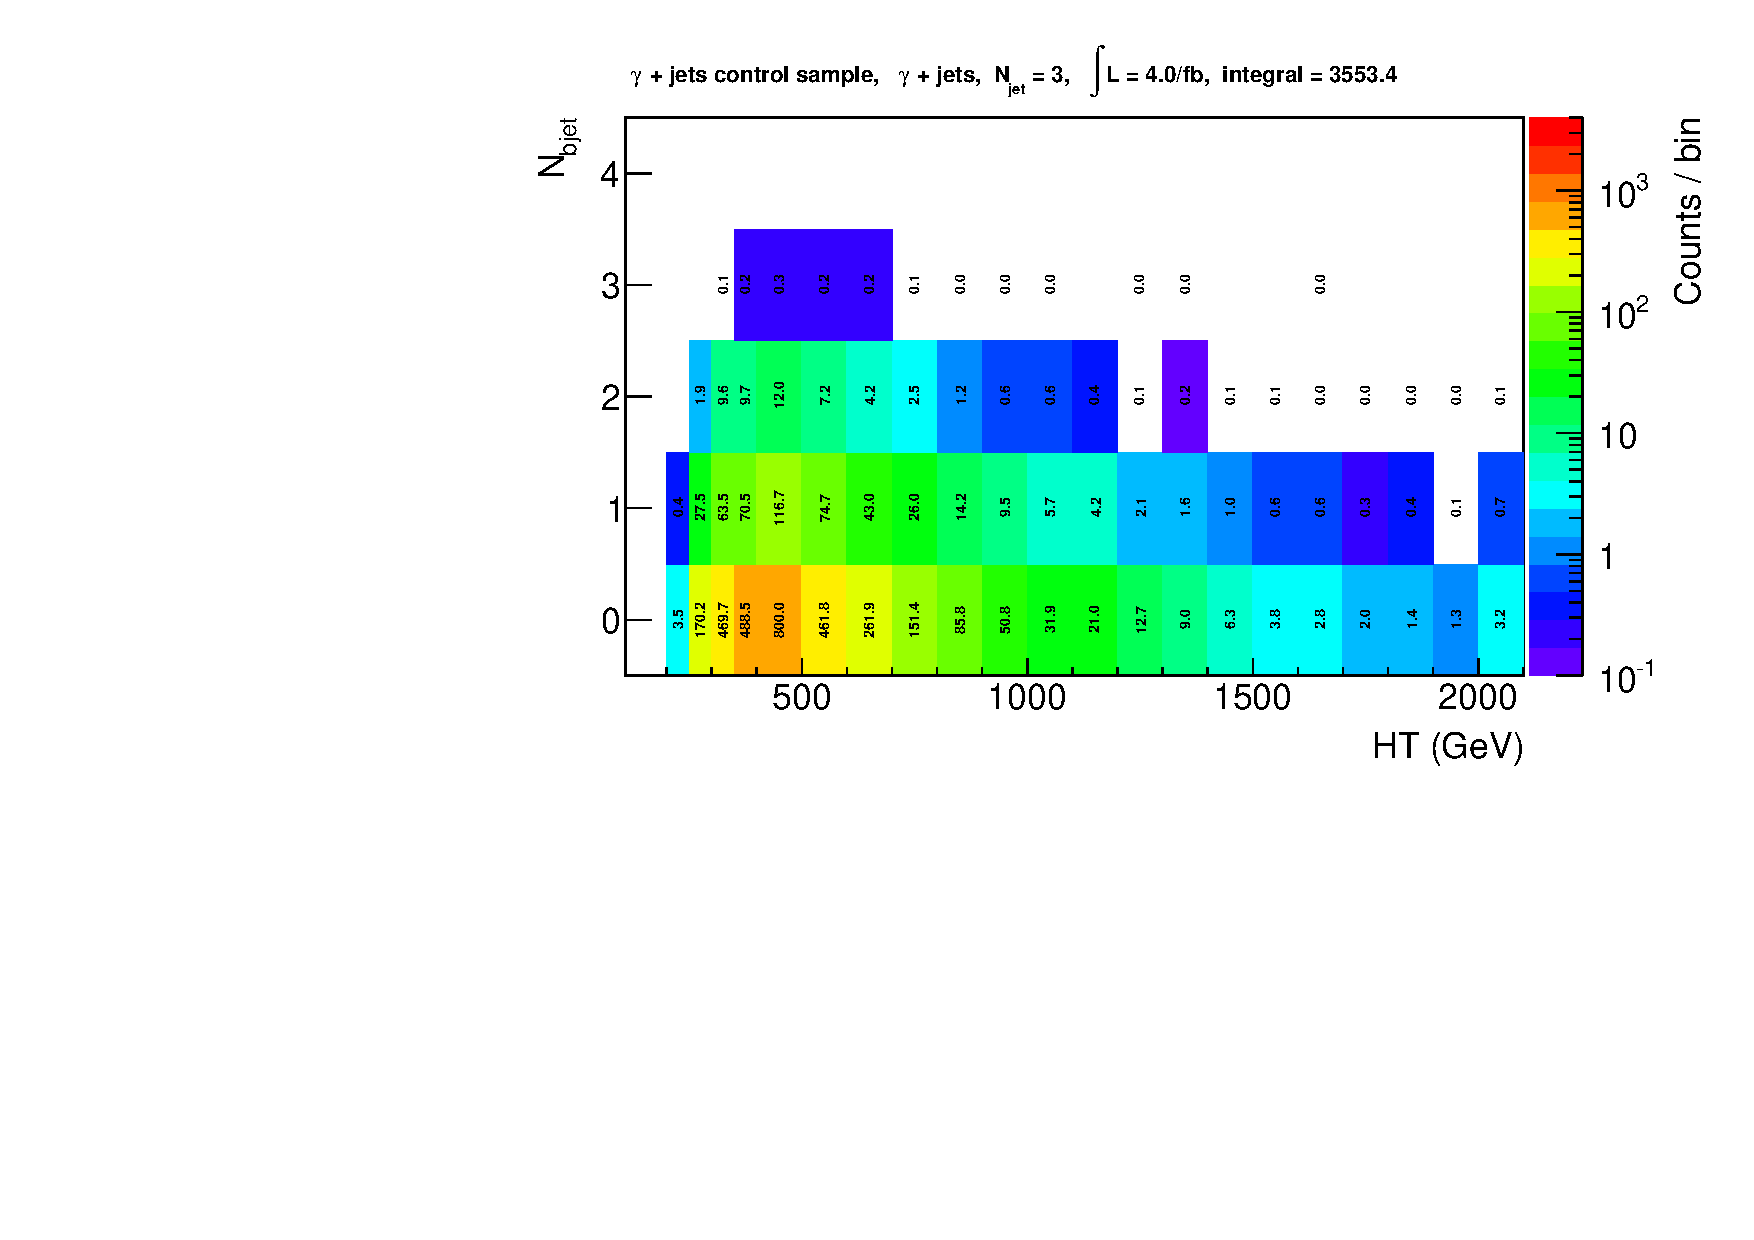
\includegraphics[width=0.5\textwidth]{figures/yieldPlots/ph_gjets_eq3j.pdf}
  }
  \\
  \subfigure[Yields from \texorpdfstring{\gj}{photon plus jets} control sample
  ($\njet = 4$)]{
    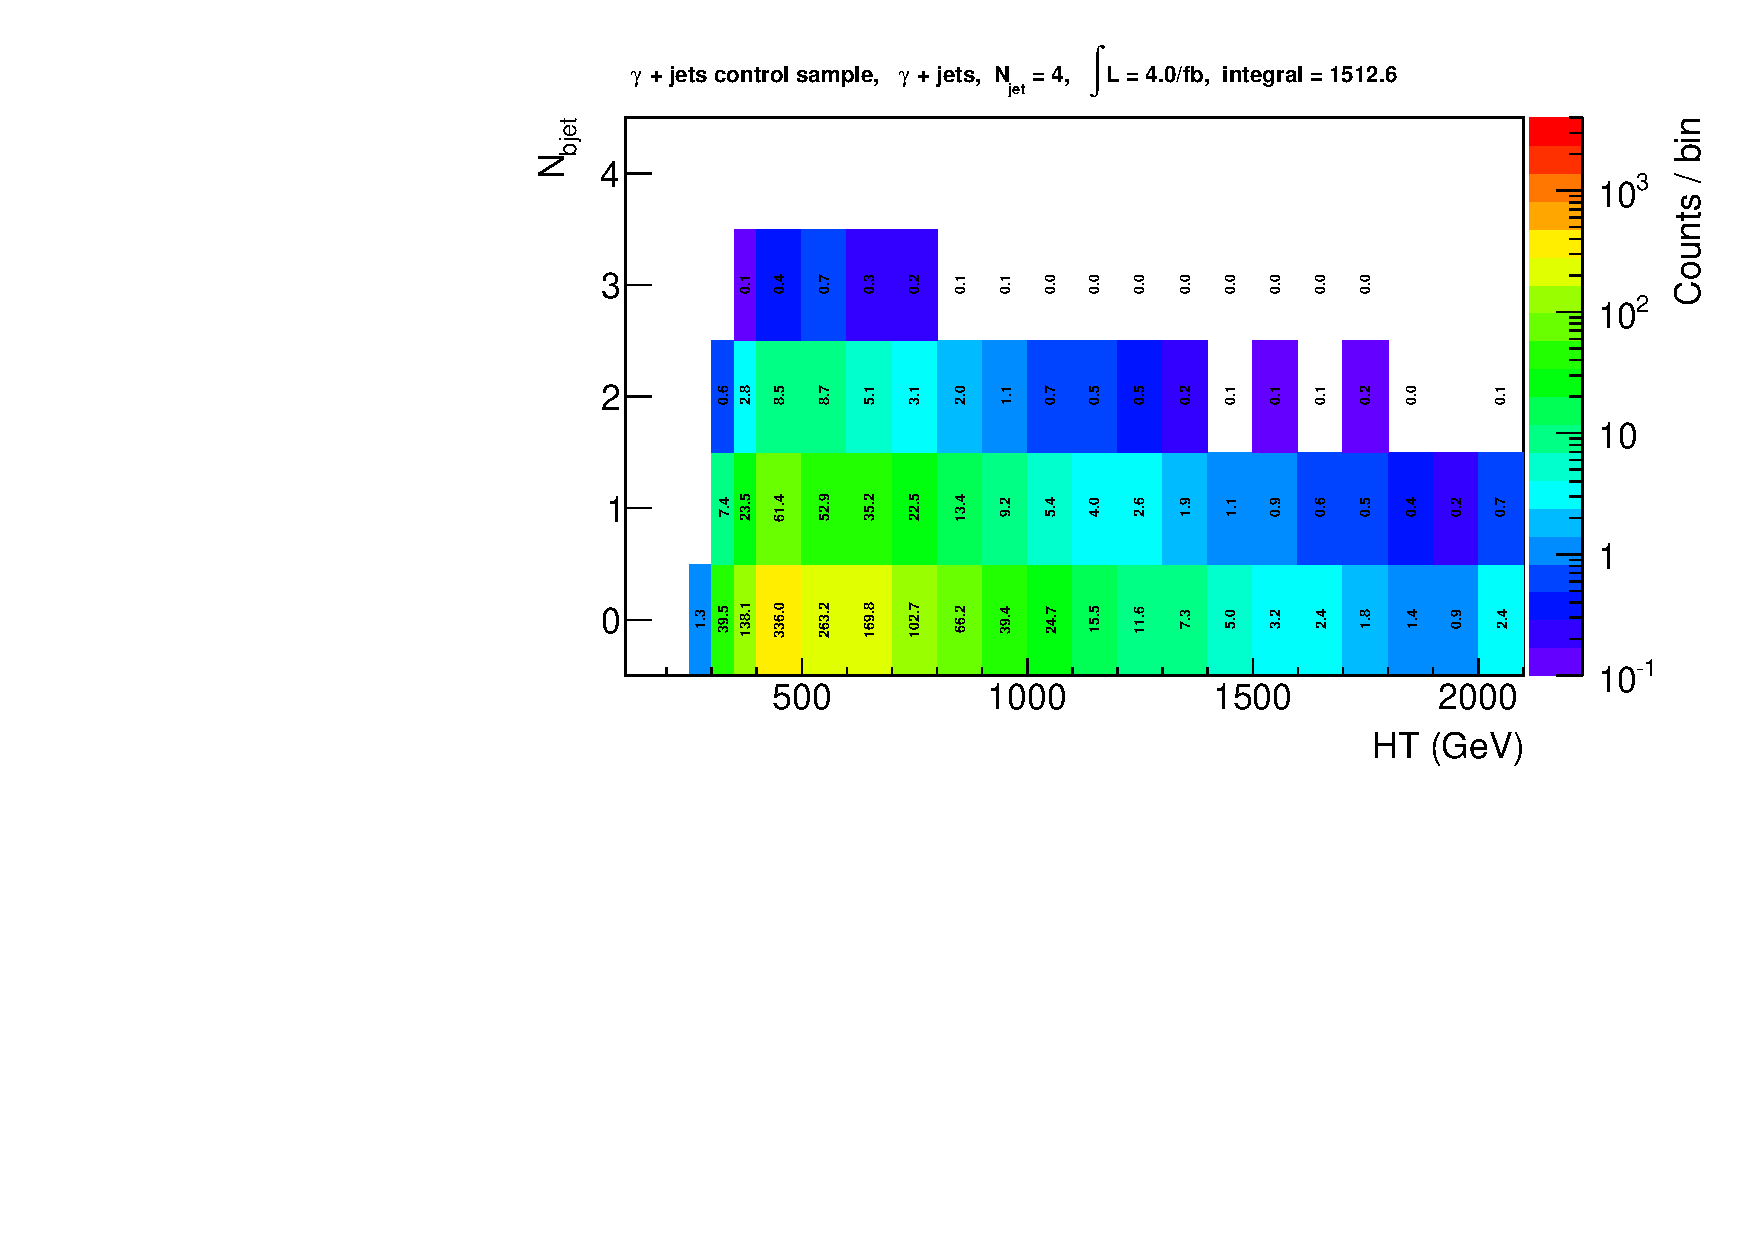
\includegraphics[width=0.5\textwidth]{figures/yieldPlots/ph_gjets_eq4j.pdf}
  }~~
  \subfigure[Yields from \texorpdfstring{\gj}{photon plus jets} control sample
  ($\njet \geq 5$)]{
    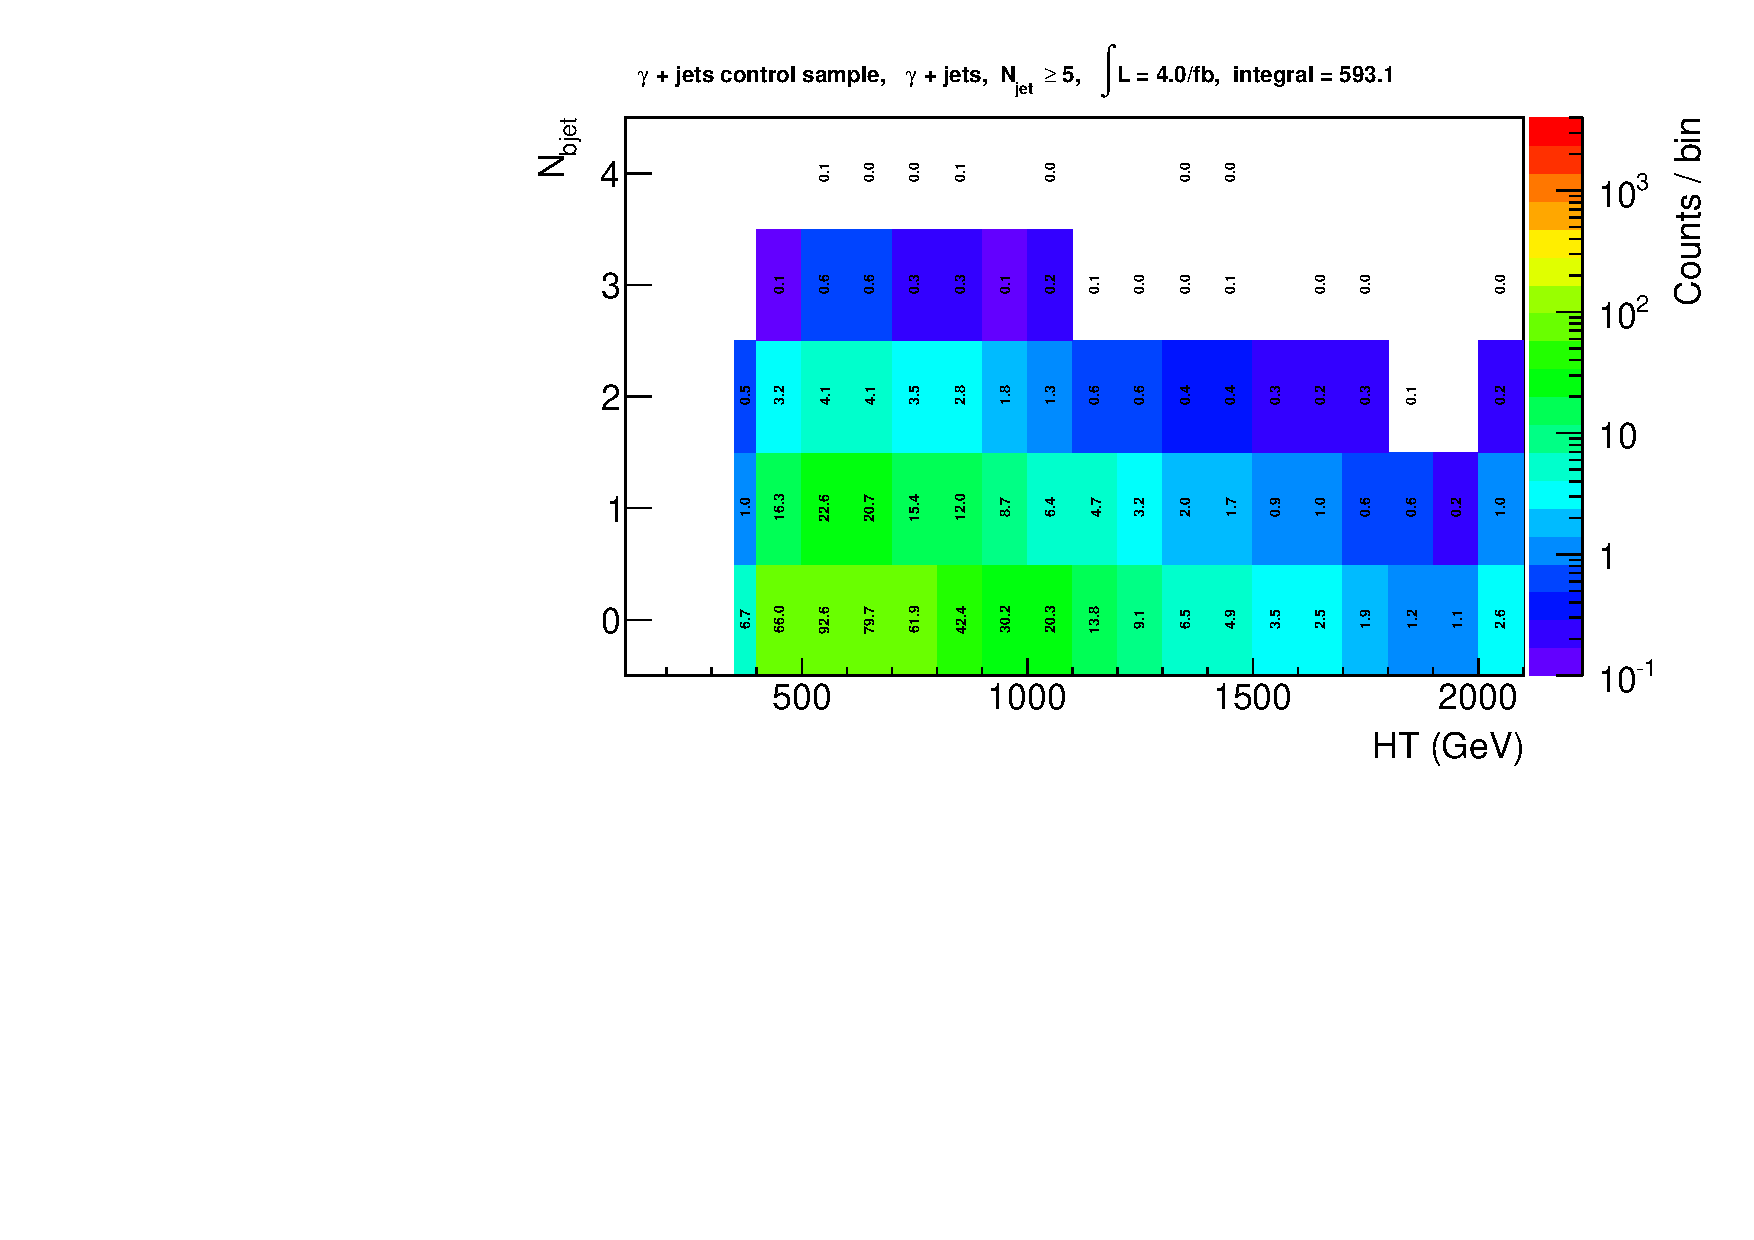
\includegraphics[width=0.5\textwidth]{figures/yieldPlots/ph_gjets_ge5j.pdf}
  } 
  \\
  \caption{\label{fig:ewkYields} Yields at $4\fbinv$ for the \gamma~+~jets MC 
  contributions to the \texorpdfstring{\gj}{photon plus jets} control sample. }
\end{figure}


%%____________________________________________________________________________||
\subsection{Future developments in the acceptance of the control samples\label{sec:larger}}
EGM-14-001 - tight to medium
%Add electron control sample

%%____________________________________________________________________________||

%%____________________________________________________________________________||
\section{Background estimation}
\label{sec:background}

\subsection{Estimation for QCD multijet events}
\subsubsection{Introduction}

A large proportion of background events is from QCD mulitjet production, due to the large cross sections and lack of precise theoretical
predictions for the cross sections and kinematic properties of multijet events. With respect to this, the approach of this analysis, like in the previous analysis, is to suppress the multijet background to a negligible level over the goal of high efficiency for any given signal model.
 
Any contamination from QCD multijet events is controlled primarily through the \alphat variable, which is able to distiguish with high efficiency the sources of ``fake'' \met, such as jet energy mismeasurement, from those with ``genuine'' \met, such as neutrinos. Any residual leakage from QCD multijet production is removed with an additional ``\met cleaning'' cut: $\mhtmet < 1.25$, which ensures that any soft jets below the $\Et$ threshold do not contribute significantly to our estimator of missing transverse energy, \mht.

In the previous analysis a conservative cut of $\alphat > 0.65,0.6,0.55$ was applied. Possibilities to loosen the \alphat cut, especially in high \scalht are being investigated. This aims at increasing the acceptance of heavy-gluino model at high \scalht. QQTAG Importantly, the signal region is defined such that the contribution from QCD multijet events is expected to be {\it negligible}. Specifically, the required level of suppression is considered sufficient for any potential QCD multijet contribution to be negligible with respect to, and absorbed fully by, the systematic uncertainties on the SM processes for which significant genuine \met is expected, predominantly V + jets and \ttbar. The requirement on \alphat is explained in Section~\ref{sec:selection}.

Thus the dominant backgrounds in the signal region are processes in which genuine \met is present in the final state, as expected from W + jets, \ttbar, and \znunu\ + jets.

The method used to determine the \alphat threshold is described below, in Section~\ref{sec:qcd-method}.

\subsubsection{Method}
\label{sec:qcd-method}
This method uses both the events passing and failing the requirement $\mhtmet < 1.25$ to estimate the number of QCD multijet events. The \alphat threshold is set such that the number of QCD multijet events is at sub-percent level to the expected contribution from EWK processes. The method comprises the following steps.

\begin{enumerate}
\item\label{item:data} A data sample rich in QCD multijet events is
  collected with the (prescaled) \httrigger triggers; this sample is
  defined by the full signal region selection criteria (defined in
  Section~\ref{sec:selection}) except for the requirements on \alphat
  and \mhtmet; the event counts, $N^{\rm data}_{i,j}$, are binned
  according to \alphat (bin $i$) and \mhtmet (bin $j$).
\item\label{item:mj} A second data sample rich in \mj events is
  collected; this sample
  is defined by the full \mj control region selection criteria
  (defined in Section~\ref{sec:def-control-samples}) with no
  requirements on \alphat and \mhtmet; the event counts,
  $n^{\mu}_{i,j}$, are binned according to \alphat (bin $i$) and
  \mhtmet (bin $j$), identical to the sample defined above.
\item\label{item:ewk} The contribution, $n^{\rm EWK}_{i,j}$ from the
  sum of all EWK processes in the QCD-enriched sample is estimated per
  bin ($i,j$) in \alphat and \mhtmet from the EWK-enriched \mj sample
  using {\it transfer factors} obtained from simulation following the
  method described in the next section
\item\label{item:qcd} The EWK contribution is subtracted from the data
  counts in the QCD-enriched sample to obtain an estimate for the QCD
  multijet contribution per bin, \ie $n^{\rm QCD}_{i,j} = n^{\rm
    data}_{i,j} - n^{\rm EWK}_{i,j}$.
\item Two bins in \mhtmet are considered: bin $j=0$ corresponds to
  events that satisfy the signal region requirement $\mhtmet < 1.25$,
  and bin $j=1$ corresponds to the inverted requirement $\mhtmet >
  1.25$. With this binning, an estimate for the number of QCD multijet
  events that pass and fail the \mhtmet requirement is determined as a
  function of the \alphat bin $i$ as follows: $R_{i}^{\mhtmet} =
  n^{\rm QCD}_{i,0} / n^{\rm QCD}_{i,1}$.
\item\label{item:ratio} The ratio $R_{i}^{\mhtmet}$ is parameterised
  by an exponentially falling function of \alphat. A fit to the ratios
  obtained from data within the range $0.505 < \alphat < 0.545$ is
  performed separately for each signal region bin defined in terms of
  \njet, \nb, and \scalht and is used to extrapolate to higher values
  of \alphat. An estimate for the number of QCD multijet events with
  \alphat above a threshold value corresponding to bin $k$ can be
  determined by taking the product of the fit expectation and the QCD
  estimate in the \mhtmet sideband bin ($i,1$) for each bin $i$ and
  summing over all bins where $i \geq k$ as follows: $N^{\rm QCD}_{k}
  = \sum\limits^{\infty}_{i=k} R_{i}^{\mhtmet} \cdot n^{\rm
    QCD}_{i,1}$.
\item The QCD multijet prediction is determined as a function of the
  threshold on \alphat (\ie as a function of bin $k$).
\item The \alphat threshold value used to defined the signal region is
  chosen such that the prediction for the QCD background is at the
  sub-percent level with respect to the corresponding expected
  contribution from EWK processes: $N^{\rm QCD}_{k} \lesssim 0.01
  \cdot N^{\rm EWK}_{k}$.
\end{enumerate}

Further data-driven studies are carried out to determine the \alphat threshold properly and reduce contributions from QCD multijets events to a negligible level in the signal region, while remaining sufficient sensitivity.

\subsection{Estimation for processes with genuine \met}
\subsubsection{Introduction}
The remaining backgrounds in the signal region, after the imposition of \alphat and \mhtmet cuts, are from SM processes with genuine \met. The main backgrounds include \znunu\ + jets, W + jets, Z + jets, \ttbar. Contributions from SM processes such as single-top, Drell-Yan, and diboson production are also expected.

To estimate the contributions from these backgrounds, three data control sample are used, which are binned identically to the signal region: $\mu$ + jets, $\mu\mu$ + jets and $\gamma$ + jets. Their definitions are in \ref{sec:selection}. $\mu\mu$ + jets and $\gamma$ + jets control sample are used to estimate the irreducible background \znunu + jets events, while $\mu$ + jets control sample is used to estimate all other SM processes. The selection criteria for these control regions are defined such that any potential contaminations from SUSY models and QCD multijets are negligible.


\subsubsection{Method}
\label{sec:ewk-method}
The method to estimate these SM background contributions relies on the use of a transfer factor. A transfer factor is the ratio of the yields obtained from MC simulation, defined for each \scalht, $n_{jet}$, $n_b$ bin of a control sample:
\begin{equation}
  \label{equ:tf-ratio}
  {\rm TF} = \frac{N_{\rm MC}^{\rm signal}(\scalht,\njet,\nb)}{N_{\rm
      MC}^{\rm control}(\scalht,\njet,\nb)} 
\end{equation}

where $\npre^{\rm signal}(\scalht,\njet,\nb)$ is the predicted yield for the corresponding bin of the signal region, and $\npre^{\rm control}(\scalht,\njet,\nb)$ is the one for the control region.

By this transfer factor, the ``na\"ive'' prediction for the total SM background can be calculated, with $\nobs^{\rm control}(\scalht,\njet,\nb)$ by:

\begin{equation}
  \label{equ:pred-method}
  \npre^{\rm signal}(\scalht,\njet,\nb) = \frac{N_{\rm MC}^{\rm
      signal}(\scalht,\njet,\nb)}{N_{\rm MC}^{\rm
      control}(\scalht,\njet,\nb)} \times \nobs^{\rm
    control}(\scalht,\njet,\nb)   
\end{equation}

When constructing the transfer factors, the MC expectations for the following SM processes are considered: W + jets ($N_{\rm W}$), \ttbar + jets ($N_{\ttbar}$), \znunu\ + jets ($N_{\znunu}$), DY + jets ($N_{\mathrm DY}$), \gj ($N_\gamma$), single top + jets production via the s, t, and tW-channels ($N_{\rm top}$), and WW + jets, WZ + jets, and ZZ + jets ($N_{\rm di-boson}$). Details on the MC samples used are given in Sec.~\ref{sec:datasets}. All MC samples are normalised to the intergrated luminosity.

The selection criteria for the three control samples closely resemble those for the signal region, differing mainly through the use of a muon, di-muon, or photon {\it tag} (that is ignored in the calculation of jet-based kinematic variables such as \scalht, \mht, \alphat, \etc) and some minimal additional kinematic requirements (\eg invariant or transerve mass windows) to obtain W, Z, and \ttbar-enriched event samples. The same selection criteria are designed to suppress signal contamination in the control samples so that unbiased data-driven estimates for the SM backgrounds in the signal region can be made. More detail on the selection criteria can be found in Section \ref{sec:selection}.

Many systematic effects are expected to cancel largely in the transfer factor. However, a systematic uncertainty is assigned to each transfer factor to account for theoretical uncertainties and effects such as the mismodelling of kinematics (\eg acceptances) and instrumental effects (\eg reconstruction efficiencies).

%%____________________________________________________________________________||

%%____________________________________________________________________________||
\section{Search sensitivity}
\label{sec:sensitivity}
\subsection{Likelihood model}

Consider a given category of event as defined by \njet and \nb.

%%%%%%%%%%%%%%%%%%%%%%%%%%%%%%%%
\subsubsection{Hadronic sample}
\label{sec:hadronicLikelihood}
%%%NOTE - MUST CHANGE SYSTEMATICS WHEN DECIDED HOW TO PROPERLEY DEAL WITH THEM!!!!!
Let $N$ be the number of bins of \HT, which need not have equal width.
Let $n^i$ represent the number of events observed satisfying all
selection requirements in each \HT bin $i$.  Then the likelihood of
the observations is written this way:

\begin{equation}
L_{hadronic}=\prod_i \mathrm{Pois}(n^i |\, b^i + s^i)
\label{eq:hadronicLikelihood}
\end{equation}

where $b^i$ represents the expected Standard Model background in bin
$i$, $s^i$ represents the expected number of signal events in bin $i$,
and $\mathrm{Pois}$ represents the Poisson distribution.  It is
assumed that:

\begin{equation}
  b^i\equiv \ewk^i
  \label{eq:ewkTotal}
\end{equation}

where $\ewk^i$ is the expected yield of electroweak events in bin $i$.
By construction, the contribution from QCD events is expected to be negligible, 
Sec.~\ref{sec:qcd}



%%%%%%%%%%%%%%%%%%%%%%%%%%%%%%%%
\subsubsection{Electroweak control samples\label{sec:ewk}}

Let \fZinv{i} represent the expected yield from \znunu in bin $i$
divided by the expected electroweak background $\ewk^{i}$.  It is
a floating parameter limited between zero and one.

Let:

\begin{equation}
  \zInv{i} \equiv \fZinv{i} \times \ewk^i 
  \label{eq:ZinvEwk}
\end{equation}

\begin{equation}
  ttW^{i} \equiv (1-\fZinv{i})\times \ewk^i
  \label{eq:ttWEwk}
\end{equation}

The variable $\zInv{i}$ thus represents the expected number of \znunu
events in \HT bin $i$ of the hadronically selected sample, and the
variable $ttW^i$ represents the expected number of events from SM
$W$-boson production (including top quark decays) in \HT bin $i$ of
the hadronically selected sample.

In each bin $i$ of \HT, there are three measurements: $n_{ph}^i$,
$n_{\mu}^i$, and $n_{\mu\mu}^i$, representing the event counts in the
photon, single-muon, and double-muon control samples.  Each of these
measurements has a corresponding yield in simulated data: $MC_{ph}^i$,
$MC_{\mu}^i$, and $MC_{\mu\mu}^i$.  The simulation also gives expected
amounts of $\zInv{}$ and $t\bar{t}+W$ in the hadronically-selected
sample: $MC_{\zInv{}}^i$ and $MC_{t\bar{t}+W}^i$.  After defining

\begin{equation}
r_{ph}^i = \frac{MC_{ph}^i}{MC_{\zInv{}}^i};\, r_{\mu\mu}^i =
\frac{MC_{\mu\mu}^i}{MC_{\zInv{}}^i};\, r_{\mu}^i =
\frac{MC_{\mu}^i}{MC_{t\bar{t}+W}^i}\quad ,
\end{equation}

these likelihood functions are used:

\begin{equation}
\label{eq:photonLikelihood}
L_{ph}= \prod_i \mathrm{Pois}(n_{ph}^i |\, \rho_{phZ}^j \cdot
r_{ph}^{i} \cdot \zInv{i})
\end{equation}

\begin{equation}
\label{eq:mumuLikelihood}
L_{\mu\mu}=\prod_i \mathrm{Pois}(n_{\mu\mu}^i |\, \rho_{\mu\mu Z}^j
\cdot r_{\mu\mu}^{i} \cdot \zInv{i})
\end{equation}

\begin{equation}
\label{eq:muonLikelihood}
L_{\mu}=\prod_i \mathrm{Pois}(n_{\mu}^i |\, \rho_{\mu W}^j \cdot
r_{\mu}^{i} \cdot ttW^{i} + s_{\mu}^i)\quad .
\end{equation}

Equation~\ref{eq:photonLikelihood} can be used to estimate the maximum
likelihood value for $\zInv{i}$ (the expectation for the \znunu\ +
jets background in the hadronic signal region) given the observations
$n_{ph}^i$ in the photon control sample and the ratios $r_{ph}^i$. A
similar construction is used when estimating $\zInv{i}$ from the
di-muon control sample (Equ.~\ref{eq:mumuLikelihood}) and $ttW^{i}$
from the single muon control sample
(Equ.~\ref{eq:muonLikelihood}). The measurements in each of the
control samples and the hadronic signal region, along with the ratios
$r_{ph}^{i}$, $r_{\mu\mu}^{i}$, and $r_{\mu}^{i}$, are all considered
simultaneously through the relationships defined in
Equs.~\ref{eq:ewkTotal}, \ref{eq:ZinvEwk}, and
\ref{eq:ttWEwk}. The ratios $r_{ph}^{i}$, $r_{\mu\mu}^{i}$, and
$r_{\mu}^{i}$ are simply the inverse of the translation factor (1/TF)
defined in Equ.~\ref{equ:pred-method}
(Sec.~\ref{sec:background-method}). More specifically, $MC_{ph}^i$,
$MC_{\mu}^i$, and $MC_{\mu\mu}^i$ are the yields obtained from MC
after applying the selection criteria for the photon, single muon and
di-muon samples, as defined by Equ.~\ref{equ:ratio-denom}
(Sec.~\ref{sec:background-method}). The variables $MC_{t\bar{t}+W}^i$ and
$MC_{\zInv{}}^i$ are defined by Equs.~\ref{equ:ratio-numer-mj} and
\ref{equ:ratio-numer-mmj} (Sec.~\ref{sec:background-method}), respectively.

The parameters $\rho_{phZ}^j$, $\rho_{\mu\mu Z}^j$, and $\rho_{\mu
  W}^j$ represent ``correction factors'' that accommodate the
systematic uncertainties associated with the control-sample-based
background constraints.  The quantities $\sigma_{phZ}^j$,
$\sigma_{\mu\mu Z}^j$, and $\sigma_{\mu W}^j$ represent the relative
systematic uncertainties for the control sample constraints, taken
into account with the following terms:

\begin{equation}
\label{eq:ewkSyst}
L_{\rm EWK\, syst.}=\prod_j \mathrm{Logn}( 1.0 |\,\rho_{\mu W}^j,
\sigma_{\mu W}^j)\times \mathrm{Logn}( 1.0 |\,\rho_{\mu\mu Z}^j,
\sigma_{\mu\mu Z}^j)\times \mathrm{Logn}( 1.0 |\,\rho_{phZ}^j,
\sigma_{phZ}^j) \quad ,
\end{equation}

where Logn is the log-normal
distribution~\cite{cousins-log-normal}:

\begin{equation}
\label{eq:log-normal}
\mathrm{Logn}(x |\,\mu,\sigma_{\mathrm{rel.}}) =
\frac{1}{x\sqrt{2\pi}\ln{k}}\exp{\left(-\frac{\ln^2{\left(\frac{x}{\mu}\right)}}{2\ln^2{k}}\right)};\quad
k=1+\sigma_{\mathrm rel.}\quad. 
\end{equation}

Seven (resp. one) parameters per control sample are used to span up to
eleven (resp. four) \HT bins, as shown in Table~\ref{tab:systMap}.

\begin{table}\centering
\caption{The systematic parameters used in \HT bins.  Left: categories
  with up to eleven bins; right: category with four bins.}
\label{tab:systMap}
\footnotesize
\begin{tabular}{lccccccccccc}
\hline
\hline
\HT bin ($i$)         & 0 & 1 & 2 & 3 & 4 & 5 & 6 & 7 & 8 & 9 & 10 \\
\hline
syst. parameter ($j$) & 0 & 1 & 2 & 3 & 3 & 4 & 4 & 5 & 5 & 6 & 6 \\
\hline
\hline
\end{tabular} \ \ 
\begin{tabular}{lccccc}
\hline
\hline
\HT bin ($i$)         & 0 & 1 & 2 & 3\\
\hline
syst. parameter ($j$) & 0 & 0 & 0 & 0\\
\hline
\hline
\end{tabular}
\end{table}

\newcommand{\rpi}{\ensuremath{r_{\mu}^{\prime\ i}}\xspace}

Alternatively, the single muon sample can be used to constrain the
total EWK background thus:

\begin{equation}
\rpi \equiv \frac{MC_{\mu}^i}{MC_{t\bar{t}+W+\zInv{}}^i}\quad ;
\end{equation}
\begin{equation}
\label{eq:muonLikelihoodTotalEwk}
L_{\mu}=\prod_i \mathrm{Pois}(n_{\mu}^i |\, \rho_{\mu W}^j \cdot
\rpi \cdot \ewk^{i} + s_{\mu}^i)\quad .
\end{equation}

The photon and di-muon likelihoods are dropped, as are the parameters
\fZinv{}.

%%%%%%%%%%%%%%%%%%%%%%%%%%%%%%%%
\subsubsection{Contributions from signal}
\label{sec:signalContrib}

Let $x$ represent the cross section for a particular signal model, and
let $l$ represent the recorded luminosity.  Let $\epsilon^{i}_{had}$
(resp.  $\epsilon^{i}_{\mu}$) be the analysis efficiency as simulated
for the model in \HT bin $i$ of the hadronic (resp. single muon
control) sample.  Let $\delta$ represent the relative uncertainty on
the signal yield, assumed to be fully correlated among the bins, and
let $\rho_{sig}$ represent the ``correction factor'' to the signal
yield which accommodates this uncertainty.  Let $f$ represent an
unknown multiplicative factor on the signal cross section, for which
an allowed interval shall be determined.

Then the expected hadronic signal yield $s^i$ from
Equation~\ref{eq:hadronicLikelihood} is written as $s^i \equiv
f\rho_{sig} xl\epsilon_{had}^i$, and the ``signal contamination'' in
the muon control sample $s_{\mu}^i$ from
Equation~\ref{eq:muonLikelihood} is treated analogously: $s_{\mu}^i
\equiv f\rho_{sig} xl\epsilon_{\mu}^i$.  The systematic uncertainty on
the signal efficiency is included via an additional term in the
likelihood:

\begin{equation}
L_{sig}=\mathrm{Logn}(1.0 |\,\rho_{sig}, \delta) \quad .
\end{equation}

%%%%%%%%%%%%%%%%%%%%%%%%%%%%%%%%
\subsubsection{Total likelihood}
\label{sec:totalLikelihood}

The likelihood function for a given selection $k$ is the product of
the terms described in the previous sections:

\begin{equation}
L^k = L_{hadronic}^k \times L_{\mu}^k \times L_{ph}^k \times
L_{\mu\mu}^k\times L_{\rm EWK\, syst.}^k \quad .
\end{equation}

In a category with 11 \HT bins and three control samples (single muon,
di-muon, and photon), there are 40 nuisance parameters:
$\{\ewk^{i}\}_{i=0}^{10}$, $\{\fZinv{i}\}_{i=0}^{10}$, $\rho_{phZ}^j$
(with $j=3,4,5,6$), $\rho_{\mu\mu Z}^j$, $\rho_{\mu W}^j$, (with
$j=0,1,2,3,4,5,6$).  In a category with eight \HT bins and one control
sample (single muon), there are 18 nuisance parameters (drop
$\{\fZinv{i}\}_{i=0}^{10}$, $\rho_{phZ}^j$, $\rho_{\mu\mu Z}^j$).  In
a category with three \HT bins and one control sample (single muon),
there are five nuisance parameters: $\ewk^{0,1,2,3}$, $\rho_{\mu
  W}^0$.  When considering signal, there is also the parameter
$\rho_{sig}$; when multiple categories are fit simultaneously, the
total likelihood is


\begin{equation}
L = L_{sig}\times \prod_k L_{hadronic}^k
\times L_{\mu}^k \times L_{ph}^k \times L_{\mu\mu}^k \times L_{\rm EWK\, syst.}^k \quad .
\end{equation}

\subsection{Signal models and efficiencies\label{sec:signal}}
To interpret the results of this search, simplified
models~\cite{Alwall:2008ag,Alwall:2008va,sms} are used. These
effective models use only a limited set of sparticles (production and
decay) and enable comprehensive studies of individual SUSY event
topologies. The simplified model studies can be performed in terms of
fundamental properties such as decay modes, production cross sections,
and sparticle masses. As gluinos provide an early discovery potential, the model
T1bbbb is used here to demonstrate sensitivity.

Signal efficiency times acceptance is determined per model per event
category (\njet,\nb) per \scalht bin. Systematic
uncertainties on the signal efficiencies are determined per model
following the 2012 analysis (see Section~\ref{sec:sms-syst}). Due to CPU
limitations, only a subset of event categories (but all \scalht bins
within a category) are considered for interpretation with each
simplified model. 

%The efficiency time acceptance for an inclusive

%selection on \scalht and for the relevant categories are shown.
The simplified models considered for the Phys14 exercise are summarised in
Table~\ref{tab:simplified-models}. The event categories considered for
each model interpretation are listed. The choice of which categories
is made by comparing the expected upper limit on the signal cross section 
per model mass point achieved for each individual event category. 
The categories are then ranked according to their expected (exclusion) reach 
and the most sensitive categories are used. 

%The second method is based on a signal
%injection test that highlights the expected signal significance per
%signal region bin. The event categories that demonstrate the largest
%significances across all \scalht bins are chosen. The former method is
%presently used.

\begin{table}[h!]
  \caption{A summary of the simplified models considered for
    interpretation. The event categories considered for each model are
    listed.}  
  \label{tab:simplified-models}
  \setlength{\extrarowheight}{2.5pt}
  \centering
  \begin{tabular}{ llcc }
    \hline
    \hline
    Model                   & Production/decay mode & (\njet,\nb) event categories considered        \\ 
    \hline
    \texttt{T1bbbb}           & \Tonebbbb               & (4,2),(4,3),(4,4),($\geq 5$,2), ($\geq 5$,3),($\geq 5$,$\geq 4$) \\ % (2--3,1), 
    % \texttt{T2bw (x=0.25)}  & \Ttwobw               & FIXME: ANA-CATS \\
    % \texttt{T2bw (x=0.75)}  & \Ttwobw               & FIXME: ANA-CATS \\
    % \texttt{T2tt}           & \Ttwott               & FIXME: ANA-CATS \\
    \hline
    \hline
  \end{tabular}
\end{table}
\subsection{Efficiency times acceptance for \texttt{T1bbbb}\label{sec:t1bbbb-eff}}

Table ~\ref{tab:simplified-models} shows the
expected signal efficiency times acceptance for the signal region and
\mj control sample (\ie, signal contamination) for the model
\texttt{T1bbbb} in the four most sensitive (\njet,\nb) event categories.
An inclusive selection on \scalht ($>200\gev$) is used. 
[CHOOSE ME]. 

\begin{table}[h!]
  \caption{A summary of the simplified models considered for
    interpretation. The event categories considered for each model are
    listed.}  
  \label{tab:simplified-models}
  \setlength{\extrarowheight}{2.5pt}
  \centering
  \begin{tabular}{ llcc }
    \hline
    \hline
    Category    & Efficiency times acceptance\\
    \hline
    (4,2)	& $0\%$	\\
    (4,3)	& $0\%$	\\
    (4,4)	& $0\%$	\\
    ($\geq 5$,2)& $0\%$	\\
    ($\geq 5$,3)& $0\%$	\\
    ($\geq 5$,$\geq 4$)	&$0\%$	\\ % (2--3,1), 
    \hline
    \hline
  \end{tabular}
\end{table}

The efficiencies are typically around $5\%$ ($~25\%$ total). Get final results on this soon.
Suggests we will be able to make a very good limit.
The signal efficiency in the \mj control sample is
negligible with respect to the signal region. By extension, the
relative contamination for the \mmj sample is also considered to be
negligible. Regardless, any potential contamination is accounted for
in the likelihood model.

\subsection{Systematic uncertainties on signal efficiency times}


For the Phys14 exercise the systematic uncertainty for the signal region 
is assumed to be unchanged from that in the previous analysis. 
Thus a systematic uncertainty of $15\%$ is applied. The systematic 
uncertainty in the signal acceptance times efficiency is determined per mass 
point per event category (\njet,\nb) per
\scalht bin (inclusive on $\scalht > 200$). The effect of
uncertainties on the luminosity measurement, the parton distribution
functions, the jet energy scale, initial state radiation, and the
efficiencies of various cuts (including the \mht/\met filter, the
``dead ECAL'' filter, etc)
%and the lepton/photon vetoes)
used in the candidate signal event selection are considered. Each
contribution is considered to be independent and all contributions are
summed in quadrature to obtain a total systematic uncertainty per mass
point per category per \scalht bin. 

\subsection{Results}


\begin{figure}[h!]
  \begin{center}
      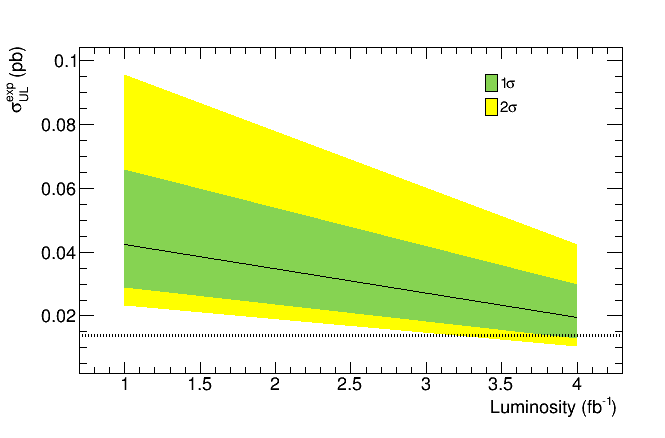
\includegraphics[width=0.8\textwidth]{figures/limit} % lbrt
      %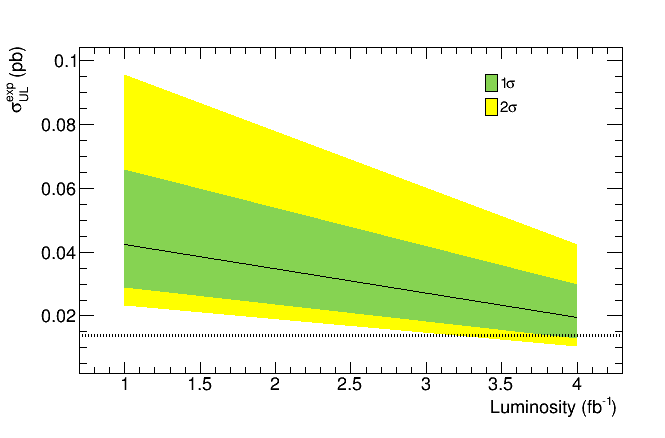
\includegraphics[width=0.45\textwidth, trim=0 190 290 20, clip=true ]{figures/limit} % lbrt
  \end{center}
 \caption{Limit at 1 and 4 fb for \texttt{T1bbbb}}
     \label{fig:limit}
\end{figure}
Assuming a systematic uncertainty of $0.15$ on the signal and taking the systematic
uncertainties on the backgrounds as $0.10$ (\scalht 200-600), $0.20$ (\scalht 600-1000),
$0.30$ (1000-$\inf$). The \scalht bins used were motivated as detailed in ???. Using the 
likelihood model from \ref{sec:hadronicLikelihood} and the \mj control sample (as $\nb > 1$) 
a limit was found for the \texttt{T1bbbb} model for luminosities of 1 and 4 fb. This is shown along 
with the theoretical cross section in \ref{fig:limit}. At 4fb it can be seen that we exclude to 1 million sigma.



%Comment to let me make a commit called first draft



%%____________________________________________________________________________||

%%____________________________________________________________________________||
\section{Summary}
\label{sec:summary}

We report on the prospects for missing energy plus jet searches that are very sensitive to 
 models of Supersymmetry and Dark Matter. The analysis follows an inclusive approach designed to 
capture a wide scope of possible final states, use of robust methods to be insensitive to multijet production,
instrumental effects and MC mis-modelling. Thus making it ideal for early data discoveries.

The proven Run I analysis concept has been extended to larger values of $H_\textrm{T}$ while also adding a new event category,
the asymetric jet selection. This selection uses an orthogonal requirement on the sub-leading jet to improve 
acceptance for ISR and monojet-type final states. This increases the acceptance of compressed SUSY models by about a factor of three
and DM models as much as a factor of five.

All signal selections region are binned according to the number of reconstructed jets, the scalar sum of the
transverse energy of jets, and the number of jets identified to originate from bottom quarks. The
sum of standard model backgrounds per bin has been estimated from a simultaneous binned
likelihood fit to event yields in the signal region and $\mu$ + jets, $\mu\mu$ + jets, and $\gamma$ + jets control sam-
ples. 

The addition of simplified and heavy quark flavored DM models yields to strong results on DM models in the spin-dependent and spin-independent nucleon cross section scattering plane in a largely model-independent way. These results may provide the strongest constraints with early 13~TeV data for low mass Dark Matter and the strongest collider constraints across a wide range of masses. In particular probe excesses observed in direct detection experiments at energies of about 10 GeV but also by the Fermi-LAT (2013) satellite indicating a DM particle of about 50 GeV mass. We expect to conclusively probe this region with the full Run II dataset.


The analysis also has been adapted to latest standards of the CMS collaboration. All analysis tools have been ported and verified using the \textsc{PHYS14} prescription in {\tt cmgtools}, the use of calojet off- and online has been replaced by particle flow (PF) jet and the trigger requirements have been adapted to maintain 2012 thresholds.
Further plans for this analysis will be to improve/increase the analysis binning for large $H_\textrm{T}$, improve and maintain trigger thresholds using PF trigger paths and evolve the selection according to the running conditions with increasing luminosity.

%\begin{itemize}
%  \item summarize the PHYS14 exercise described in the other sections
%  \item mention briefly further preparation plans for Run 2
%  \item conclude with the outlook for Run 2
%\end{itemize}

%%____________________________________________________________________________||


%%____________________________________________________________________________||
